% Sample Dissertation, Thesis, or Document %
%            for use with the              %
%  University of Arizona Thesis Class,     %
%               uathesis.cls               %
%------------------------------------------%

% We'll use the uathesis document class (duh).  The uncommented line
% below will produce a Dissertation, the others would produce a Thesis
% or a Document.  There are other options available to you like turning
% on the copyright statement and replacing the year on the title page
% with a "generated on" stamp (handy for early drafts).  To find out
% what the available options are, take a look into the uathesis.cls
% file and look for the \DeclareOption commands near the top of that
% file.
% There are five copyright options.  Copyright, no copyright, and three
% different Creative Commons licences.  Use the one you want (If you go
% Creative Commons, I (DM) think the CC-BY-ND makes the most sense)  See
% uathesis.cls for the reason why the non-commercial licenses are not
% included.
\documentclass[dissertation]{uathesis}
%\documentclass[dissertation,copyright]{uathesis}
%\documentclass[dissertation,CC-BY]{uathesis}
%\documentclass[dissertation,CC-BY-SA]{uathesis}
%\documentclass[dissertation,CC-BY-ND]{uathesis}
%\documentclass[thesis]{uathesis}
%\documentclass[document]{uathesis}

% Package Usage
% These are the packages that we need
\usepackage{graphicx}
\usepackage{natbib}			% natbib is available on most systems, and is
					% terribly handy.
					% If you want to use a different Bibliography package, 
					% you should be able to, just change this
					% and the \bibliographystyle command below.  Be warned
					% that you may need to do a little hacking to get
					% the REFERENCES item to show up in your TOC.

% Compatibility with the AASTEX package 
% of the American Astronomical Society.
% I COMMENTED OUT LINE 150 OF DELUXETABLE.STY
\usepackage{deluxetable}		% Allows use of AASTEX deluxe tables
\usepackage{aastex_hack}		% Allows other AASTEX functionality.


% These are other packages that you might find useful.
% For controlling the fonts, see
% http://www.math.uiuc.edu/~hartke/computer/latex/survey/survey.html
% The following is a nice font set:
%\usepackage{mathtime}			% Times for letters; Belleek math.
%
\usepackage{amsmath}			% AMS Math (advanced math typesetting)
\usepackage{amssymb} 
\usepackage{lscape}			% Used for making fitting large tables in by putting them landscape
\usepackage[tableposition=t]{caption} % NICK ADDED THIS (makes table captions normal size when font set smaller)

%%% Evan added the following
\usepackage{mathtools}
\usepackage{bm}
\usepackage{enumitem}
\usepackage{units} % includes nicefrac

% My packages
\usepackage[colorlinks=true,linkcolor=blue,citecolor=cyan]{hyperref}
\usepackage{pdfpages}
%\usepackage[numbers]{natbib}
\usepackage{authblk}
\usepackage{caption}
%\usepackage{subcaption}
\usepackage{graphicx}
\usepackage{amsmath}
\usepackage{amssymb}
\usepackage{epstopdf}
\usepackage{comment}
\usepackage{xcolor}
\usepackage{float}
\usepackage{doi}
\usepackage{tikz-feynman}
\tikzfeynmanset{compat=1.1.0}

% Useful macros for equations and units in HEP
\newcommand*{\TeV}{\text{ TeV}}
\newcommand*{\GeV}{\text{ GeV}}
\newcommand*{\MeV}{\text{ MeV}}
\newcommand*{\keV}{\text{ keV}}
\newcommand*{\eV}{\text{ eV}}
\newcommand*{\meV}{\text{ meV}}
\newcommand*{\bb}{\boldsymbol}
\newcommand*{\beqn}{\begin{equation}}
\newcommand*{\eeqn}{\end{equation}}
\newcommand{\req}[1]{Eq.\,(\ref{#1})}
\newcommand{\rf}[1]{Fig.~{\ref{#1}}}
\newcommand{\rsec}[1]{Sect.\,{\ref{#1}}}

% Useful macros for annotation
\newcommand*{\xred}{\color{red}}
\newcommand*{\xblue}{\color{black}}
\newcommand*{\xgreen}{\color{green}}

%%% The following allows dagger footnote on chapter titles
%%% with no number. Useful for designating previously 
%%% published work.
\newcounter{daggerfootnote}
\newcommand*{\daggerfootnote}[1]{%
    \setcounter{daggerfootnote}{\value{footnote}}%
    \renewcommand*{\thefootnote}{\fnsymbol{footnote}}%
    \footnote[2]{#1}%
    \setcounter{footnote}{\value{daggerfootnote}}%
    \renewcommand*{\thefootnote}{\arabic{footnote}}%
    }

\newcommand{\Msun}{\mathrm{M}_{\odot}}
%\usepackage{refs}			
%
% If you are using hyper-ref (recommended), this command must go after all 
% other package inclusions (from the hyperref package documentation).
% The purpose of hyperref is to make the PDF created extensively
% cross-referenced.
%\usepackage[hidelinks]{hyperref}


% Set up some values.
\completetitle{Fundamental applications of relativistic classical and quantum magnetism}
\fullname{Andrew James Steinmetz}			% Grad college wants your full name here.
\degreename{Doctor of Philosophy}	% Title of your degree.
\degreemajor{Physics} % Degree major
\begin{document}


% Set up the title page
\maketitlepage
{DEPARTMENT OF PHYSICS}	% Title of your department.
{2023}							

% Insert the approval form.  Note that for electronic submission
% of your Ph. D. dissertation, you must bring *two* copies of the
% approval page to your final defense.  These must be signed by
% the committee.  Make two photocopies: one for Pam and the other
% for your records.  Then, bring the two signed originals to the
% graduate college when you submit the final version of the
% dissertation to the University of Arizona.
\approval
{}		% Defense Date	
{}	% Dissertation Director
{}	% 1st committee member
{}		% 2nd committee member
{}		% 3rd committee member
{}		% 4th committee member
{}		% 5th committee member
{}		% 6th committee member

% Include the ``Statement by Author'' for Dissertations
\statementbyauthor
% If this is a Thesis, use the following form, with your thesis director's
% name and title in the square brackets like so (you should also omit the 
% approval form insertion above):
%\statementbyauthor[Jane M. Doe\\Professor of Chemistry]

% Include the ``Acknowledgements''
\incacknowledgements{acknowledgements}

% Include the ``Dedication''
\incdedication{dedication}

% Create a ``Table of Contents''
\tableofcontents

% Create a ``List of Figures''
\listoffigures

% Create a ``List of Tables''
\listoftables

% Include the ``Abstract''
\incabstract{00abstract}

% Include the various chapters
%%%%%%%%%%%%%%%%%%%%%%%%%%%%%%%%%%%%%%%
\chapter{Introduction and overview}
\label{chap:intro}
%%%%%%%%%%%%%%%%%%%%%%%%%%%%%%%%%%%%%%%
\noindent This chapter serves to introduce and motivate the fundamental concepts of spin, magnetic moment and electromagnetism which will be explored in the subsequent chapters. This chapter will also serve to establish notation conventions. The classical and quantum formulations of spin will be defined in \rsec{sec:spin} in both relativistic and non-relativistic contexts. In \rsec{sec:mom} we will introduce magnetic (and electric) dipoles and the concept of anomalous magnetic moments (AMM) which have played a crucial role in physics. A list of relevant publications with author contributions is outlined in \rsec{sec:pubs}.

%%%%%%%%%%%%%%%%%%%%%%%%%%%%%%%%%%%%%%%
\section{The importance of spin}
\label{sec:spin}
%%%%%%%%%%%%%%%%%%%%%%%%%%%%%%%%%%%%%%%
Rotation and spin are ubiquitous phenomenon found in nearly every aspect of physics and has played an important role in establishing quantum mechanics in the 20th century due to its quantized nature. In relativistic mechanics, spin angular momentum is one of two Casimir invariants (with the other invariant being mass) of the Poincar{\'e} group of spacetime symmetry transformations (rotations, boosts, and translations). Each particle in relativistic mechanics is characterized by its mass and spin.

All fundamental particles known in physics have a non-zero spin angular momentum with the exception of the Higgs boson which is a scalar with spin-0. All other fundamental particles (such as electrons, quarks, photons, etc...) have values of either spin-1/2 or spin-1. Particles with even values of spin are known as bosons while half-integer particles with spin are called fermions. Composite particles have have even more exotic spin values and fundamental particles which higher spins such as 3/2 are common in beyond-standard-model physics.

%%%%%%%%%%%%%%%%%%%%%%%%%%%%%%%%%%%%%%%
\subsection{Quantum spin}
\label{sec:qspin}
%%%%%%%%%%%%%%%%%%%%%%%%%%%%%%%%%%%%%%%

%%%%%%%%%%%%%%%%%%%%%%%%%%%%%%%%%%%%%%%
\section{Quantum magnetic dipoles}
\label{sec:mom}
%%%%%%%%%%%%%%%%%%%%%%%%%%%%%%%%%%%%%%%
In classical theory, when charges rotate or circulate in some manner, a magnetic field is produced characterized by the magnetic dipole moment of the system. This concept can be transplanted into quantum theory. The natural size of the magnetic moment of a particle (in this context a lepton) is given by the magneton value
\begin{align}
    \label{mag:1}
    \mu_{\ell}\equiv\frac{e\hbar}{2m_{\ell}}
\end{align}
where the lepton (denoted by $\ell$) has charge $e$ and mass $m_{\ell}$. For electrons, this quantity is referred to as the Bohr magneton. As quantum mechanics is not well described in terms of forces or accelerations (except in the context of Ehrenfest-style equations), there is no simple operator companion for torque. However, the expression for the non-relativistic energy can be written down in terms of a Hamiltonian operator. In quantum mechanics, the 3-spin operator for a spin-1/2 particle is defined as
\begin{align}
    \label{qspin:1}
    \bb{ s}=\frac{\hbar}{2}\bb{\sigma}
\end{align}
where $\bb{\sigma}$ are the familiar $2\times2$ Pauli matrices. The magnetic dipole Hamiltonian is given by
\begin{align}
	\label{mag:2}
    {H}_{\mathrm{Mag}}=-\bb{\mu}\cdot\bb{B}\,,\\
    \bb{\mu}=g\frac{e\hbar}{2m_{\ell}}\frac{\bb{\sigma}}{2}=g\mu_{\ell}\frac{\bb{\sigma}}{2}\,,
\end{align}
where $\bb{\mu}$ is the magnetic moment operator defined in terms of the Pauli matrices. The parameter $g$ is the gyromagnetic ratio (or g-factor) of the particle. The \lq natural\rq\ value for $g$ (as predicted by the Dirac equation) is $g=2$. When $g\neq2$, which is true for all physical particles, the anomalous magnetic moment (AMM) can be defined via 
\begin{align}
    \label{amm:1}
    a\equiv\frac{g}{2}-1\,,\\
    \label{amm:2} a\frac{e\hbar}{2m_{\ell}}\rightarrow\delta\mu\equiv\mu-\mu_{\ell}\,,
\end{align}
where $a$ is the anomaly parameter. We also introduce $\delta\mu$ as the anomalous magnetic moment magnitude.

We note that $g\mu_{\ell}$ in \req{mag:2} can be either positive or negative depending on the sign of the charge which is the convention followed by CODATA. \req{mag:2} is the operator equivalent of the single particle magnetization energy described classically as
\begin{align}
    \label{mag:3}
    U=-\bb{\mu}\cdot\bb{B}
\end{align}

Just like the classical situation, the anomalous magnetic moment coupling $a$ is then responsible for deviations from the \lq natural\rq\ magnetic moment. In non-relativistic quantum mechanics, the charged Schrodinger-Pauli Hamiltonian ${ H}_{\rm SP}$ is then given by
\begin{align}
	\label{sp:1}
    {H}_{\mathrm{SP}}\ \chi=\left(\frac{1}{2m_{\ell}}\bb{\pi}^{2}-\bb{\mu}\cdot\bb{B}+e{ V}\right)\psi=i\hbar\frac{\partial}{\partial t}\chi\,,\\
    \bb{\pi}\equiv\bb{ p}-e{\bb{A}}\,,
\end{align}
where $\chi$ is a two-component spinor. Using SI units, the four-potential is written as $A^{\alpha}=\left(V/c,\bb{A}\right)^{T}$. The relativistic generalization of \req{sp:1} is the Dirac equation. It is well known that \req{sp:1} is obtainable from the Dirac equation in the non-relativistic limit which famously predicts $g=2$ for the magnetic dipoles of fermions. The process can be done economically (Sakurai, 1967) using an ansatz of large and small components. This method however loses usefulness for higher order corrections producing imaginary contributions to the Hamiltonian. This was resolved first by (Foldy, 1950) using what is now known as the Foldy-Wouthuysen (FW) transformation. This procedure will be briefly discussed in \rsec{ajss:quantclass}.

%%%%%%%%%%%%%%%%%%%%%%%%%%%%%%%%%%%%%%%
\section{Ehrenfest theorem for Stern-Gerlach forces}
%%%%%%%%%%%%%%%%%%%%%%%%%%%%%%%%%%%%%%%
\noindent The relativistic precession of a spin-1/2 particle can be extracted from the Dirac equation. The Dirac equation with electromagnetic interaction is given by
\begin{alignat}{1}
  \label{DIRAC01} i\hbar\frac{\partial}{\partial t}\psi=\left(\boldsymbol{\alpha}\cdot\left(\mathbf{p}c-e\mathbf{A}\right)+eA_{0}+\gamma^{0}mc^{2}\right)\psi=\hat{H}_{D}\psi\,,
\end{alignat}
where we will use the conventions
\begin{alignat}{1}
  \label{DIRAC02} \boldsymbol{\alpha}=\gamma^{0}\boldsymbol{\gamma},\indent\boldsymbol{\Sigma}=\gamma_{5}\boldsymbol{\gamma},\indent\gamma_{5}=i\gamma^{0}\gamma^{1}\gamma^{2}\gamma^{3},\indent\gamma_{5}^{2}=1\,.
\end{alignat}
From the Heisenberg equations of motion
\begin{alignat}{1}
  \label{DIRAC03} i\hbar\frac{\mathrm{d}\hat{O}}{\mathrm{d}t}=[\hat{O},\hat{H}]+i\hbar\frac{\partial\hat{O}}{\partial t}\,,
\end{alignat}
the operator spin precession is
\begin{alignat}{1}
  \label{DIRAC04} \frac{\mathrm{d}\mathbf{S}_{R}}{\mathrm{d}t}=\frac{\mathrm{d}}{\mathrm{d}t}\left(\frac{\hbar}{2}\boldsymbol{\Sigma}\right)=-\boldsymbol{\alpha}\times\left(\mathbf{p}c-e\mathbf{A}\right)\,,
\end{alignat}
where $\mathbf{S}_{R}$ is the relativistic spin operator. While this expression is fully relativistic, it is not easily interpreted due to the off-diagonal nature of the $\boldsymbol{\alpha}$ matrices which mix particle and antiparticle components. A similar situation arises for the \lq\lq velocity operator\rq\rq\, which leads to the phenomenon of \emph{Zitterbewegung}. Eq.~\eqref{DIRAC04} reveals that spin is not a constant of motion of the Dirac equation. The orbital angular momentum $\mathbf{L}$ is also not a constant of motion, but the sum of the two or the total angular momentum $\mathbf{J}$ is.

%%%%%%%%%%%%%%%%%%%%%%%%%%%%%%%%%%%%%%%
\subsection{Foldy-Wouthuysen transformation}
%%%%%%%%%%%%%%%%%%%%%%%%%%%%%%%%%%%%%%%
To connect the relativistic quantum notion of spin to our non-relativistic classical intuition we need to disentangle the components of the Dirac equation. To do this we make use of the Foldy-Wouthuysen (FW) transformation which diagonalizes odd operators via a unitary transformation
\begin{alignat}{1}
  \label{FW01} \psi\rightarrow\psi'=e^{i\mathcal{S}}\psi,\indent\hat{H}\rightarrow\hat{H}'=e^{i\mathcal{S}}\hat{H}e^{-i\mathcal{S}}-ie^{i\mathcal{S}}\frac{\partial e^{-i\mathcal{S}}}{\partial t}\,,
\end{alignat}
where $\mathcal{S}$ is Hermitian. The resulting Hamiltonian $\hat{H}'$ then produces two uncoupled equations of two-component spinors. For free particles the transformed Hamiltonian has an exact closed form, but for charged particles in weak fields the Hamiltonian will be an infinite series in powers of inverse mass $1/m$. Our interest lies in determining the first nonlinear terms in the spin precession of order $|\mathbf{s}|^{2}$ as these are the first terms to be sensitive to field in-homogeneity. Because of the intimate relationship between spin and magnetic moment, the expressions we seek will be up to order $\mu^{2}\sim e^{2}/m^{2}$ and thus we only require the FW transformed Hamiltonian up to $1/m^{2}$.

The generated Hamiltonian is therefore
\begin{alignat}{1}
  \notag\hat{H}'&=\gamma^{0}\left\{mc^{2}+\frac{1}{2m}\left(\mathbf{p}-\frac{e}{c}\mathbf{A}\right)^{2}-eA_{0}-\frac{e\hbar}{2mc}\boldsymbol{\sigma}\cdot\mathbf{B}\right.\\
  \notag&+\frac{e\hbar}{8m^{2}c^{2}}\boldsymbol{\sigma}\cdot\left(\left(\mathbf{p}-\frac{e}{c}\mathbf{A}\right)\times\mathbf{E}-\mathbf{E}\times\left(\mathbf{p}-\frac{e}{c}\mathbf{A}\right)\right)\\
  \label{FW02}&-\left.\frac{e\hbar^{2}}{8m^{2}c^{2}}\boldsymbol{\nabla}\cdot\mathbf{E}+\ldots\right\}\,.
\end{alignat}
The $\boldsymbol{\sigma}$ operators are simply the Pauli matrices. The first four terms represent the rest mass-energy of the particle and the Schr\"{o}dinger-Pauli (SP) Hamiltonian, the fifth term is the spin-orbit coupling, and the last is the Darwin term. In determining the precession, it is the spin Hamiltonian
\begin{alignat}{1}
  \notag\hat{H}'_{spin}=&-\frac{e\hbar}{2mc}\boldsymbol{\sigma}\cdot\bigg(\mathbf{B}\\
  \label{FW03}&-\frac{1}{4mc}\left(\left(\mathbf{p}-\frac{e}{c}\mathbf{A}\right)\times\mathbf{E}-\mathbf{E}\times\left(\mathbf{p}-\frac{e}{c}\mathbf{A}\right)\right)\bigg),
\end{alignat}
which will be relevant.

%%%%%%%%%%%%%%%%%%%%%%%%%%%%%%%%%%%%%%%
\subsection{Second order spin effects}
%%%%%%%%%%%%%%%%%%%%%%%%%%%%%%%%%%%%%%%
By substituting eq.~\eqref{FW03} into eq.~\eqref{DIRAC03}, the non-relativistic spin precession (up to order $1/m^{2}$) is found to be
\begin{alignat}{1}
  \notag\frac{\mathrm{d}\mathbf{S}_{NR}}{\mathrm{d}t}=\frac{\mathrm{d}}{\mathrm{d}t}\left(\frac{\hbar}{2}\boldsymbol{\sigma}\right)&=\frac{e\hbar}{2mc}\boldsymbol{\sigma}\times\mathbf{B}\\
  \notag&-\frac{e\hbar}{4m^{2}c^{2}}\boldsymbol{\sigma}\times\left(\mathbf{E}\times\left(\mathbf{p}-\frac{e}{c}\mathbf{A}\right)\right)\\
  \label{SPIN01}&-\frac{e\hbar^{2}}{16m^{2}c^{2}}\left[\boldsymbol{\sigma},\boldsymbol{\sigma}\cdot\left(\boldsymbol{\nabla}\times\mathbf{E}\right)\right]\,,
\end{alignat}
where $\mathbf{S}_{NR}$ is the non-relativistic spin operator. The first term is the expected Larmor precession, and the second is precession generated by spin-orbit coupling. The last term is second order in spin and sensitive to the curl of electric fields. This term cannot be easily categorized as a simple \lq\lq quantum correction\rq\rq\, as both orders of $\hbar$ are consumed by the definition of the spin operator and survive the $\hbar\rightarrow 0$ limit. This term in fact is more analogous to the $p^{4}$ correction to a particle's energy due to relativity.

As spin dynamics in quantum mechanics exhibits more complicated behavior at higher orders, due to special relativity, we expect similar corrections to appear in the classical theory of spin precession in the same manner that energy corrections appear.

%%%%%%%%%%%%%%%%%%%%%%%%%%%%%%%%%%%%%%%
\section{The naturalness of $g=2$}
\label{sec:nat}
%%%%%%%%%%%%%%%%%%%%%%%%%%%%%%%%%%%%%%%
As discussed by Feynman (Feynman, 1961), there is a strong predilection in nature towards $g=2$ gyro-magnetic factors which can be explained by the requirements of kinetic operator in quantum mechanics. We note that because the $2\times2$ Pauli matrices $\bb{\sigma}$ all anti-commute, we can write down the relation
\begin{alignat}{1}
	\label{nat:1} (\bb{\sigma}\cdot\bb{a})(\bb{\sigma}\cdot\bb{b})=\bb{a}\cdot\bb{b}+i\bb{\sigma}\cdot(\bb{a}\times\bb{b})\,.
\end{alignat}
The non-relativistic kinetic energy Hamiltonian from \req{sp:1} then reads as
\begin{alignat}{1}
	\label{nat:2} {H}_{\mathrm{KE}}=\frac{1}{2m}\left(\bb{\sigma}\cdot\bb{\pi}\right)^{2}=\frac{1}{2m}\bb{\pi}^{2}+i\bb{\sigma}\cdot(\bb{\pi}\times\bb{\pi})\,.
\end{alignat}
As the kinetic momentum operator $\bb{\pi}$ does not self-commute, its cross-product is non-zero resulting in
\begin{alignat}{1}
	\label{nat:3} {H}_{\mathrm{KE}}=\frac{1}{2m}\bb{\pi}^{2}-\frac{e\hbar}{2m}\bb{\sigma}\cdot\bb{B}\,,
\end{alignat}
which is the magnetic moment term with size $g=2$. We recognize that $g=2$ appears to arise from the $\mathfrak{su}(2)$ Lie algebra (Schultz, 1980) representation described by the Pauli matrices and electromagnetic minimal coupling. The natural scale of the magnetic moment can be interpreted as originating from group symmetry requirements on charged particles. Rather than taking the non-relativistic limit of the Dirac equation, $g=2$ can also be derived as a consequence of replacing the definition of the inner product for vectors which accounts for spin (Feynman, 1961). The Schrodinger kinetic Hamiltonian and Schrodinger-Pauli kinetic terms are then related via substitution
\begin{alignat}{1}
	\label{nat:4} \bb{\pi}\cdot\bb{\pi} \rightarrow (\bb{\pi}\cdot\bb{\sigma})(\bb{\sigma}\cdot\bb{\pi})\,.
\end{alignat}
An almost identical argument that g-factor arises from spin-structure and electromagnetic coupling can be made for the relativistic case as well. First we consider the quantum analog to the energy-momentum relation
\begin{alignat}{1}
	\label{analog:1} \eta_{\alpha\beta}p^{\alpha}p^{\beta}\Psi=m^{2}c^{2}\Psi\,.
\end{alignat}
\req{analog:1} as written evaluates to the Klein-Gordon equation when the four-momentum is written in the position basis $p^{\alpha}\rightarrow i\hbar\partial^{\alpha}$. Much like the non-relativistic example, we can introduce spin by replacing the momentum inner product with one sensitive to a Clifford algebra (Weinberg, 1995). Rather than the Pauli matrices, the relativistic replacement utilizes the gamma matrices $\eta_{\alpha\beta}\rightarrow\gamma_{\alpha}\gamma_{\beta}$ yielding
\begin{alignat}{1}
	\label{eq:spin:03} \gamma_{\alpha}\gamma_{\beta}p^{\alpha}p^{\beta}\Psi&=m^{2}c^{2}\Psi\,.
\end{alignat}
Here $\Psi$ is understood to be a four-component spinor unlike in \req{analog:1}. The corresponding $4\times4$ matrix contraction identity analog to \req{nat:1} is then
\begin{alignat}{1}
	\label{eq:spin:04} \gamma_{\alpha}\gamma_{\beta}a^{\alpha}b^{\beta}=\eta_{\alpha\beta}a^{\alpha}b^{\beta}-i\sigma_{\alpha\beta}a^{\alpha}b^{\beta}\,,\indent \sigma_{\alpha\beta}\equiv\frac{i}{2}\left[\gamma_{\alpha},\gamma_{\beta}\right]\,.
\end{alignat}
The anti-symmetric spin tensor $\sigma_{\alpha\beta}$ is defined by the commutator of the gamma matrices. In both the relativistic and non-relativistic cases, the distinction between spin-1/2 and spinless particles is only made kinematically apparent in the presence of electromagnetic fields. For minimal coupling
\begin{alignat}{1}
  \label{eq:spin:05} \pi^{\alpha}=p^{\alpha}-eA^{\alpha}\,,
\end{alignat}
we take advantage of the fact that any product can be written as a sum of commuting and anti-commuting parts
\begin{alignat}{1}
	\label{eq:spin:06} \pi^{\alpha}\pi^{\beta}=\frac{1}{2}\left(\left\{\pi^{\alpha},\pi^{\beta}\right\}+\left[\pi^{\alpha},\pi^{\beta}\right]\right)\,.
\end{alignat}
yielding
\begin{alignat}{1}
	\label{eq:spin:07a} \left(\eta_{\alpha\beta}\pi^{\alpha}\pi^{\beta}-\frac{i}{2}\sigma_{\alpha\beta}\left[\pi^{\alpha},\pi^{\beta}\right]\right)\Psi&=m^{2}c^{2}\Psi\,,\\
	\label{eq:spin:07b} \left(\eta_{\alpha\beta}\pi^{\alpha}\pi^{\beta}-\frac{e\hbar}{2}\sigma_{\alpha\beta}F^{\alpha\beta}\right)\Psi&=m^{2}c^{2}\Psi\,.
\end{alignat}
\req{eq:spin:07b} is the square of the Dirac equation with precisely $g=2$. Furthermore, compelling arguments can be made that all elementary particles (Ferrara et. al. 1992) of any spin have a natural value of $g=2$, though a competing idea is Belinfante's conjecture of $g=1/s$. To paraphrase the argument by Ferrara, Porrati and Telegdi, $g=2$ is likely the natural scale for particles of any spin because:
\begin{enumerate}
	\item The W boson, as the only known higher spin charged elementary particle, has at tree level $g=2$ via a Proca-like equation.
	\item For $g=2$, the relativistic TBMT spin equation is the same simplified form any classical spin value.
	\item For arbitrary spin, $g=2$ facilitates finite Compton scattering cross sections without additional physical requirements.
	\item For arbitrary spin, open bosonic and super-symmetric string theory predicts $g=2$.
\end{enumerate}
While the above provide a nice justification for why particles should tend to this specific g-factor, the reality is no particle has exactly $g=2$ with all of them displaying some form of anomaly. The charged leptons come the closest to the natural value, but famously have vacuum polarization contributions \cite{Schwinger:1951nm} from QED, non-perturbative hadronic contributions \cite{Jegerlehner:2001wq,Jegerlehner:2017gek}, and potentially BSM interactions \cite{Czarnecki:2001pv,Knecht:2004,Jegerlehner:2009ry} contributing to their anomalous magnetic dipole moment. There are then two major approaches to deal with anomalous moments. The first is to consider the fundamental quantum field theory describing the particle, and then analyzing the resulting tree level diagrams which contribute to the moment in a perturbative fashion. The second is to utilize an effective field theory with the anomalous moment already implemented in the base wave dynamics. While the first approach has proven to be exceedingly successful for the charged leptons (the muon's anomaly notwithstanding), it is not appropriate for particles whose moments are dramatically different from $g=2$ or if the origin of the anomaly comes from internal structure such as the hadrons whose moments are determined by nonpertubative QCD \cite{Eichmann:2016yit,Pacetti:2014jai} and not vacuum structure as is the case for the nucleons and atoms.

\begin{table}
	\centering
\begin{tabular}{|r|l|}
	electron & -2.002\ 319\ 304\ 362\ 56(35)\\
	muon & -2.002\ 331\ 8418(13)\\
	tau & \ -2.036(34)\\
	proton & \ 5.585\ 694\ 6893(16)\\
	neutron & -3.826\ 085\ 45(90)\\
	deuterium & \ 0.857\ 438\ 2338(22)\\
	tritium & \ 5.957\ 924\ 931(12)
\end{tabular}
	\caption{The g-factor PDG values of various particles. Of those listed, only the tau is poorly measured and whose anomaly is not well constrained. As a general rule, composite particles deviate from $g=2$ greatly. Comparing the three isotopes of hydrogen shows how magnetic moments can \lq\lq cancel\rq\rq\ out so that while deuterium differs great from the proton, tritium with two neutrons does not and is similar.}
	\label{ajs:table:01}
\end{table}

%%%%%%%%%%%%%%%%%%%%%%%%%%%%%%%%%%%%%%%
\section{Construction of classical spin}
\label{sec:cspin}
%%%%%%%%%%%%%%%%%%%%%%%%%%%%%%%%%%%%%%%
The classical 3-spin is given by
\begin{align}
    \label{cspin:1}
    \vec{s}=(s_{x},\ s_{y},\ s_{z})^{\rm T}
\end{align}

%%%%%%%%%%%%%%%%%%%%%%%%%%%%%%%%%%%%%%%
\section{Publications and author contributions}
\label{sec:pubs}
%%%%%%%%%%%%%%%%%%%%%%%%%%%%%%%%%%%%%%%

\chapter{Classical magnetic dipole moments}
    \section{Stern-Gerlach force}
        \subsection{Amperian and Gilbert dipoles}
    \section{TBMT equations}
    \section{Magnetic spin potential}
%\\\\\\\\\\\\\\\\\\\\\\\\\\\\\\\\\\\\\\\\\\\\\\\\\\\\\\\\\\\\\\\\\\\\\\\\\\\\\\\\\\\\\\\\\\\\\\\\\\\\\\\\\\\\\\\\\\\\\\\\\\\\\\\\\\\\\\\\\\\\\\%
In classical theory, we consider the covariant dipole force which acts upon a particle due to its intrinsic magnetic moment. The generalized covariant Lorentz and dipole force is given by
\begin{alignat}{1}
  \label{LSG01} m\frac{\mathrm{d}u^{\alpha}}{\mathrm{d}\tau}&=eF^{\alpha\beta}u_{\beta}+dG^{\alpha\beta}u_{\beta}\,,\\
  \label{LSG02} G^{\alpha\beta}&=\partial^{\alpha}F^{*\beta\gamma}s_{\gamma}-\partial^{\beta}F^{*\alpha\gamma}s_{\gamma}\,,
\end{alignat}
where $e$ and $d$ are the electric and dipole charges, and $F^{*}$ is the electromagnetic dual tensor. While the first term in equation~\eqref{LSG01} is the standard Lorentz force, the second term is a covariant formulation of the Stern-Gerlach (SG) force. Because the spin precession is sensitive to the force on a particle, the presence of a SG force will induce precession terms which are second order in spin. The generalized spin precession that corresponds to eq.~\eqref{LSG01} is therefore
\begin{alignat}{1}
  \notag\frac{\mathrm{d}s^{\mu}}{\mathrm{d}\tau}&=(1+\tilde{a})\frac{e}{m}F^{\mu\nu}s_{\nu}-\tilde{a}\frac{e}{m}u^{\mu}\left(u_{\alpha}F^{\alpha\beta}s_{\beta}\right)/c^{2}\\
  \label{LSG03}&+(1+\tilde{b})\frac{d}{m}G^{\mu\nu}s_{\nu}-\tilde{b}\frac{d}{m}u^{\mu}\left(u_{\alpha}G^{\alpha\beta}s_{\beta}\right)/c^{2}\,.
\end{alignat}
The constants $\tilde{a}$ and $\tilde{b}$ are arbitrary allowing for extra terms not forbidden by special relativity. In the standard derivation of relativistic spin precession, in the form of the TBMT equation, the $\tilde{a}$ constant is associated with the anomalous magnetic moment. In allowing for spin precession sourced by a Stern-Gerlach dipole force, an additional constant $\tilde{b}$ must be introduced. The terms in eq.~\eqref{LSG02} involving the $G$ tensor are spin precession directly originating from dipole forces. In homogeneous electromagnetic fields, eq.~\eqref{LSG02} reduces to the standard TBMT equation.

        \subsection{Modified TBMT equations}
        \subsection{Unified Amperian and Gilbert dipoles}
        \subsection{Dynamic particle motion}
            \subsubsection{Charged particles}
            \subsubsection{Neutral particles}
%%%%%%%%%%%%%%%%%%%%%%%%%%%%%%%%%%%%%%%
\chapter{Quantum magnetic dipole moments}
%%%%%%%%%%%%%%%%%%%%%%%%%%%%%%%%%%%%%%%
\section{Schrodinger-Pauli equation}\label{ajss:quantumdipole}
\noindent One of the striking lessons of strong field electrodynamics is the difference of the spin-0 Klein-Gordon and spin-1/2 Dirac energy levels, and their ordering, around a Coulomb center. As free Dirac particles solutions are also solutions to the Klein-Gordon equation, this discrepancy must originate from the presence of spin and consequently dipole moment.


\section{Dirac and Dirac-Pauli equations}\label{ajsss:diracpauli}
The most straight-forward manner to generalize the magnetic moment for relativistic fermions is to add a Pauli term to the Dirac equation proportional to the anomalous portion. While in most texts, the moment is given in terms of g-factor \lq\lq$g$\rq\rq\ or the anomaly \lq\lq$a$\rq\rq\ we wish to keep our equations general to particles of any given charge $e$ and magnetic moment $\mu$.

We then consider the substitution
\begin{alignat}{1}
	\label{eq:diracpauli:01a} a\frac{e\hbar}{2m_{\ell}}\longrightarrow\delta\mu\equiv\mu-\mu_{\ell}\,,
\end{alignat}
where $\mu_{\ell}$ is the lepton magneton as previously defined. The Dirac-Pauli (DP) equation then reads as
\begin{alignat}{1}
	\label{eq:diracpauli:01b} \left(\gamma_{\alpha}(i\hbar\partial^{\alpha}-eA^{\alpha})-m_{\ell}c-\delta\mu\frac{1}{2c}\sigma_{\alpha\beta}F^{\alpha\beta}\right)\psi=0\,,
\end{alignat}
where the spin tensor is defined as
\begin{alignat}{1}
	\label{eq:diracpauli:02} \sigma_{\alpha\beta}=\frac{i}{2}\left[\gamma_{\alpha},\gamma_{\beta}\right]\,.
\end{alignat}
The wave function $\psi$ here is then a four-component spinor. When the anomalous part is zero, the standard Dirac equation is recovered. For charged leptons, the Pauli term can be understood to be a vacuum contribution which modifies the photon 3-vertex. This term can be further expressed as
\begin{alignat}{1}
	\label{eq:diracpauli:03} \frac{1}{2}\sigma_{\alpha\beta}F^{\alpha\beta}=\frac{i}{c}\bb{\alpha}\cdot\bb{E}-\bb{\Sigma}\cdot\bb{B}\,,
\end{alignat}
which captures that relativistic magnetic moments should be sensitive to electric as well as magnetic fields. This should be unsurprising if one considers how the non-relativistic dipole form must generalize under Lorentz boost. The Pauli term also informs how to construct the generalized electric dipole. The generalization to include the electric dipole is
\begin{alignat}{1}
	\label{eq:diracpauli:04} \delta\mu\rightarrow\delta\tilde{\mu}\equiv\delta\mu+i\epsilon\gamma^{5}\,,
\end{alignat}
where $\epsilon$ is the electric dipole of the lepton. As the natural electric dipole within the Dirac equation is zero, the presence of $\epsilon$ is always considered anomalous. We will use the following conventions throughout the remainder of the report
\begin{alignat}{1}
	\label{eq:diracpauli:05} \bb{\alpha}=\gamma_{0}\bb{\gamma}\,,\indent \bb{\Sigma}=\gamma_{5}\bb{\alpha}\,,\indent \gamma_{5}=i\gamma_{0}\gamma_{1}\gamma_{2}\gamma_{3}\,,\indent \gamma^{2}_{5}=1\,.
\end{alignat}
Exact solutions to the DP equation are relatively scarce due to the complicating nature of the anomalous term. The most extensively studied solutions are those with high symmetries or constant external fields \cite{Thaller:2013,Bagrov:2014}.

%%%%%%%%%%%%%%%%%%%%%%%%%%%%%%%%%%%%%%%
\section{Klein-Gordon-Pauli equation}
\noindent While the DP equation is more commonly used, there exists an alternative wave equation which describes the magnetic behavior of fermions called the Klein-Gordon-Pauli (KGP) equation. This equation is physically distinct from the DP and Dirac equations and only share solutions when $g=2$. The KGP equation is generally considered to be the \lq\lq square\rq\rq\ of the Dirac equation as unlike the Dirac or DP equations, it is a second order equation given by
\begin{alignat}{1}
	\label{eq:kgp:01} \left((i\hbar\partial-eA)^{2}-m_{\ell}^{2}c^{2}-\left(\mu+i\epsilon\gamma^{5}\right)m_{\ell}\sigma_{\alpha\beta}F^{\alpha\beta}\right)\Psi=0\,.
\end{alignat}
This equation is mathematically similar to the Klein-Gordon equation which describes charged scalar particles. Because the covariant derivative is squared, the above equation results in a $e^{2}A^{2}$ term which represents the presence of a 4-vertex seagull coupling between two fermion lines and two photons to maintain charge gauge invariance. For a g-factor of $g=2$, the equation reduces to the square of the Dirac equation which is explicitly shown in \req{eq:kgp:03}. If we define the Dirac operator as
\begin{alignat}{1}
	\label{eq:kgp:02} \mathcal{D}_{\pm}=\gamma_{\alpha}(i\hbar\partial^{\alpha}-eA^{\alpha})\pm m_{\ell}c\,,\indent\mathcal{D}_{-}=-\gamma^{5}\mathcal{D}_{+}\gamma^{5}\,,
\end{alignat}
in terms of a positive and negative mass, we can complete the square of the Dirac equation via the substitution
\begin{alignat}{1}
	\label{eq:kgp:03} \mathcal{D}_{+}\psi\rightarrow\mathcal{D}_{+}\mathcal{D}_{-}\Psi\,,\indent\mathcal{D}_{+}\mathcal{D}_{-}\Psi=\left((i\hbar\partial-eA)^{2}-m_{\ell}^{2}c^{2}-\frac{e\hbar}{2}\sigma_{\alpha\beta}F^{\alpha\beta}\right)\Psi=0\,.
\end{alignat}
This procedure yields \req{eq:kgp:01} or the KGP equation for $g=2$. More generally however, the KGP equation is able to describe fermions of any arbitrary magnetic and electric moments. The KGP equation was first introduced by Fock \cite{Fock:1937dy} and more thoroughly examined by Feynman and Gell-Mann \cite{Feynman:1958ty} for weak interactions. The initial benefit of the KGP formulation is that the wave equation fully commutes with $\gamma^{5}$ making all eigenfunctions good chiral states though at the expense of more complicated parity relationships.

%%%%%%%%%%%%%%%%%%%%%%%%%%%%%%%%%%%%%%%
\subsection{KGP in homogeneous fields}\label{ajsss:homogeneous}
\noindent The case of the homogeneous magnetic field, sometimes referred to as the Landau problem, provides a stepping stone in which to examine all other consequences of quantum spin dynamics. We take a constant magnetic field in the $z$-direction to be
\begin{alignat}{1}
	\label{eq:homogeneous:01} \bb{B}=B\hat{z}\,.
\end{alignat}
For our choice of gauge, there are two common options: (a) the Landau $\bb{A}_{L}$ gauge and (b) the symmetric $\bb{A}_{S}$ gauge
\begin{alignat}{1}
	\label{eq:homogeneous:02} \bb{A}_{L}=B(0,x,0)^{T}\,,\indent \bb{A}_{S}=\frac{B}{2}(-y,x,0)^{T}\,.
\end{alignat}
As the system has a manifest rotational symmetry perpendicular to the direction of the homogeneous field, we will choose the symmetric gauge which preserves this symmetry explicitly. Before we examine relativistic wave equations, it will be helpful to first consider the non-relativistic Schrodinger-Pauli case as the non-relativistic solutions are related to the Dirac-Landau and KGP-Landau cases. In fact, the relativistic Dirac, KGP, and non-relativistic Pauli cases are mathematically equivalent. Energy eigenstates of \req{eq:quantumdipole:02} under the homogeneous field \req{eq:homogeneous:01} yields
\begin{alignat}{1}
	\label{eq:homogeneous:03} \psi=\psi_{E}\times e^{-iEt/\hbar}\,,\indent\left(\frac{1}{2m}\left(\bb{p}-e\bb{A}\right)^{2}-\mu B\sigma_{z}\right)\psi_{E}=E\psi_{E}\,,
\end{alignat}
where $\mu=|\bb{\mu}|$ is the magnitude of the magnetic moment. We can convert to the relativistic model via a substitution of the energy. \req{eq:homogeneous:03} for our specific choice of symmetric gauge \req{eq:homogeneous:02} can be rewritten as
\begin{alignat}{1}
	\label{eq:homogeneous:04} \hat{H}\psi_{E}=\left(\frac{1}{2m}\bb{p}^{2}+\frac{e^{2}B^{2}}{8m}(x^{2}+y^{2})-\frac{eB}{2m}L_{z}-\mu B\sigma_{z}\right)\psi_{E}=E\psi_{E}\,.
\end{alignat}
We note the vector potential results in a term which behaves like the potential for a quantum harmonic oscillator and a term for the orbital angular momentum in the direction of the magnetic field. These terms can be grouped into three mutually commuting independent Hamiltonian operators
\begin{alignat}{1}
	\label{eq:homogeneous:05} \hat{H}=\hat{H}_{\mathrm{HO}}+\hat{H}_{\mathrm{Free}}+\hat{H}_{\mathrm{Mag.}}\,.
\end{alignat}
Denoting the cyclotron frequency
\begin{alignat}{1}
	\label{eq:homogeneous:06} 2\omega = \omega_{c} = \frac{eB}{m}\,,
\end{alignat}
we write the three Hamiltonian operators as
\begin{subequations}
\begin{alignat}{2}
	\label{eq:homogeneous:07a} &\hat{H}_{\mathrm{HO}}&&=\frac{1}{2m}\left(p_{x}^{2}+p_{y}^{2}\right)+\frac{1}{2}m\omega^{2}(x^{2}+y^{2})\,,\\
	\label{eq:homogeneous:07b} &\hat{H}_{\mathrm{Free}}&&=\frac{p_{z}^{2}}{2m}\,,\\
	\label{eq:homogeneous:07c} &\hat{H}_{\mathrm{Mag.}}&&=-\left(\omega\bb{L}+\mu\bb{\sigma}\right)\cdot B\hat{\bb{z}}\,.
\end{alignat}
\end{subequations}
The full Hamiltonian \req{eq:homogeneous:05} then is composed of (a) the two-dimensional quantum harmonic oscillator, (b) a free kinetic term for momentum states aligned with the magnetic field and (c) the magnetic or Zeeman interaction. While \req{eq:homogeneous:07c} is usually expressed as
\begin{alignat}{1}
	\label{eq:homogeneous:07} \hat{H}_{\mathrm{Mag.}}=-\frac{e}{2m}\left(\bb{L}+g\bb{S}\right)\cdot\bb{B}\,,
\end{alignat}
with an explicit g-factor, we will prefer to keep the charged contribution separate from the moment contribution so that both charged and neutral particles can be described with minimal changes in notation. As all the above Hamiltonians are mutually commuting, the energy eigenvalue of the total Hamiltonian is the sum of the individual energy eigenvalues. 
%
%It will be helpful to introduce the following latter operators
%\begin{subequations}
%\begin{alignat}{1}
%	\label{eq:homogeneous:08a} a &= \sqrt{\frac{m\omega}{2\hbar}}\left(x+\frac{ip_{x}}{m\omega}\right)\,,\\
%	\label{eq:homogeneous:08b} b &= \sqrt{\frac{m\omega}{2\hbar}}\left(y+\frac{ip_{y}}{m\omega}\right)\,,\\
%	\label{eq:homogeneous:08c} c &= \frac{1}{\sqrt{2}}(a+ib)\,.
%\end{alignat}
%\end{subequations}
%which satisfy the following commutators
%\begin{alignat}{1}
%	\label{eq:homogeneous:09} [a,a^{\dagger}]=[b,b^{\dagger}]=[c,c^{\dagger}]=1\,,\indent [c,a^{\dagger}]=1\,,\indent [c,b^{\dagger}]=i\,,
%\end{alignat}
%with all other commutators being zero. These ladder operators raise or lower states in the usual fashion
%\begin{alignat}{1}
%	\label{eq:homogeneous:10} d^{\dagger}|n_{d}\rangle=\sqrt{n_{d}+1}|n_{d}+1\rangle\,,\indent d^{\dagger}d|n_{d}\rangle=n_{d}|n_{d}\rangle\,,\indent d\in a,b,c\,. 
%\end{alignat}
%Utilizing the ladder operators Eq.~(\ref{eq:homogeneous:08a}--\ref{eq:homogeneous:08b}) we can recast \req{eq:homogeneous:05} as
%\begin{alignat}{1}
%	\label{eq:homogeneous:11a} \hat{H}&=\frac{p_{z}^{2}}{2m}+\hbar\omega\left(1+a^{\dagger}a+b^{\dagger}b-i\left(ab^{\dagger}-a^{\dagger}b\right)\right)-\mu B\sigma_{z}\,,\\
%	\label{eq:homogeneous:11b} L_{z}&=i\hbar\left(ab^{\dagger}-a^{\dagger}b\right)\,.
%\end{alignat}
%Here we see that their is a relationship between the $x$ and $y$-direction ladder operators and the $z$-axis orbital angular momentum however the relationship is muddied until we substitute in \req{eq:homogeneous:08c} yielding
%\begin{alignat}{1}
%	\label{eq:homogeneous:12} \hat{H}&=\frac{p_{z}^{2}}{2m}+\hbar\omega_{c}\left(\frac{1}{2}+c^{\dagger}c\right)-\mu B\sigma_{z}\,.
%\end{alignat}
%\req{eq:homogeneous:12} has been reduced to the normal one-dimensional harmonic oscillator (with free $z$-momentum) modified by a spin dependent quantity. If the eigenvalues of $c^{\dagger}c$ and spin are denoted as
%\begin{alignat}{1}
%	\label{eq:homogeneous:13} \sigma_{z}|z\pm\rangle=\pm|z\pm\rangle\,,\indent c^{\dagger}c|n\rangle=n|n\rangle\,,
%\end{alignat}
%then the energy eigenvalues of \req{eq:homogeneous:12} are

Using the method of ladder operators, the energy eigenvalues of \req{eq:homogeneous:05} are found to be
\begin{alignat}{1}
	\label{eq:homogeneous:14} E(p_{z},n,s) = \frac{p_{z}^{2}}{2m}+\hbar\omega_{c}\left(\frac{1}{2}+n\right)-\mu Bs\,,\indent n\in0,1,2\ldots\,,\indent s\in\pm1\,,
\end{alignat}
where $n$ is the principle quantum number. If the magnetic moment $\mu$ is defined as the magneton of a charged particle with $g=2$, then last two terms in the above equation simplify into states defined by the Landau quantum number
\begin{alignat}{1}
	\label{eq:homogeneous:15} E(p_{z},\lambda_{L}) = \frac{p_{z}^{2}}{2m}+\hbar\omega_{c}\lambda_{L}\,,\indent\lambda_{L}\equiv\frac{1-s}{2}+n\,,\indent\lambda_{L}\in0,1,2\ldots
\end{alignat}
Landau states are double degenerate for all states above the ground state $\lambda_{L}=0$. The presence of anomalous magnetic moment then serves to break this degeneracy. This feature is true in both the non-relativistic and relativistic cases.

%%%%%%%%%%%%%%%%%%%%%%%%%%%%%%%%%%%%%%%
\subsubsection{Dirac-Pauli Case}\label{ajsss:diracpauli}
\noindent The DP \req{eq:diracpauli:01b} in this system takes on the form
\begin{alignat}{1}
	\label{eq:diracpauli:05} \left[\gamma_{\alpha}(i\hbar c\partial^{\alpha}-eA^{\alpha})-mc^{2}-a\mu_{B}\bb{\sigma}\cdot\bb{B}\right]\psi=0\,,
\end{alignat}
Its energy solutions \cite{Johnson:1950zz,OConnell:1968,Tsai:1971zma} are then given by
\begin{alignat}{1}
	\label{eq:diracpauli:06} E^{2}_{DP}=\left(\sqrt{m^{2}c^{4}+4\mu_{B}mc^{2}B\lambda_{L}}-a\mu_{B}Bs\right)^{2}+p_{z}^{2}c^{2}\,,
\end{alignat}
where $\lambda_{L}\in0,1,2,\ldots$ is the Landau level and $s\in\pm1$ is the spin quantum number defined the same way as in \rsec{ajsss:homogeneous}. Just like the non-relativistic case, the relativistic Landau states maintain a double degeneracy above the ground state for $g=2$. The anomalous magnetic moment then serves to break this degeneracy, however it does so in a rather complicated manner which results in the natural magnetic moment defined by the magneton and the anomalous moment to affect the levels in physically distinct ways. This breaks the sensibility that a magnetic dipole should physically behave the same regardless of its size. In the weak field limit, the solution connects back to the Dirac Landau energies as expected.

%%%%%%%%%%%%%%%%%%%%%%%%%%%%%
\subsubsection*{Dirac and KGP Case}\label{ajsss:DKGP}
\noindent As mentioned in \rsec{ajsss:homogeneous}, the non-relativistic Pauli system and the Dirac and KGP systems are mathematically equivalent for homogeneous fields. This allows us to pull the relativistic energy $E_{R}$ eigenvalues straight from the non-relativistic $E_{NR}$ values via the substitution and redefinition of non-relativistic mass $m_{NR}$
\begin{alignat}{1}
	\label{eq:DKGP:01} E_{NR} = \frac{E_{R}^{2}-m_{R}^{2}c^{4}}{2E_{R}}\,,\indent  E_{R} = m_{NR}c^{2}\,.
\end{alignat}
The resulting eigenvalues, dropping the relativistic subscripts, are then given by
\begin{alignat}{1}
	\label{eq:DKGP:02} E_{KGP} =\pm\sqrt{m^{2}c^{4}+p_{z}^{2}c^{2}+2e\hbar c^{2}B\left(n+\frac{1}{2}\right)\pm2\mu mc^{2}B}\,.
\end{alignat}
To obtain the Dirac levels, simply set $g=2$. In this equation, we can clearly see the energy contribution contains an orbital part, which houses the transverse $x$ and $y$-momentum, and a magnetic contribution which can either raise of lower the level. In the Dirac case, there is a degeneracy among Landau levels as in the non-relativistic case which is then broken by the presence of the anomaly.

%%%%%%%%%%%%%%%%%%%%%%%%%%%%%%%%%%%%%%%
\subsection{KGP for hydrogen-like atoms}
%%%%%%%%%%%%%%%%%%%%%%%%%%%%%
\subsubsection{Charged-Coulomb Problem}\label{ajsss:coulomb}
The Coulomb problem, or sometimes referred to as the Kepler problem, provides us with a standard application of any quantum theory to explore. As the hydrogen-like atom is the most well understood atomic system in physics, any non-minimal behavior especially for high-$Z$ systems can lead to dramatic consequences for the resulting spectra. We take the Coulomb potential to be
\begin{equation}
	\label{eq:coulomb:01} V_\mathrm{C}\equiv e A^{0}=\frac{Z \alpha\hbar c}{r}\;,\qquad \vec{A}=\vec{0}\;.
\end{equation}
The KGP-Coulomb problem can be solved analytically {\color{red}Add citation.} We will briefly sketch out the solution and its consequences. For energy states $\Psi=e^{-iEt/\hbar}\Psi_{E}$ the KGP equation yields the following differential equation
\begin{alignat}{1}
	\label{cou02} \left(\frac{E^{2}-m^{2}c^{4}}{\hbar^{2}c^{2}}+\frac{Z^{2}\alpha^{2}}{r^{2}}+\frac{2E}{\hbar c}\frac{Z\alpha}{r}+\frac{1}{r}\frac{\partial^{2}}{\partial r^{2}}r-\frac{L^{2}/\hbar^{2}}{r^{2}}-\frac{g}{2}Z\alpha\frac{i\vec{\alpha}\cdot\hat{r}}{r^{2}}\right)\Psi_{E}=0\;.
\end{alignat}
We recast the squared angular momentum operator $L^{2}$ with the Dirac spin-alignment operator
\begin{alignat}{1}
\label{cou04} &\mathcal{K}=\gamma^{0}\left(1+\bb{\Sigma}\cdot\frac{\bb{L}}{\hbar}\right)\;,\indent L^{2}/\hbar^{2}=\mathcal{K}\left(\mathcal{K}-\gamma^{0}\right)\;.
\end{alignat}
The operator $\mathcal{K}$ commutes with $\vec{\alpha}\cdot\hat{r}$ and its eigenvalues are given as either positive or negative integers $\kappa=\pm(j+1/2)$ where $j$ is the total angular momentum quantum number. By grouping all terms proportional to $1/r^{2}$, we see the effective angular momentum eigenvalues take on non-integer values which in the limit of classical mechanics corresponds to orbits which do not close. {\color{red}Add citation.} The non-integer eigenvalues depends explicitly on $g$-factor. The difficulty of this equation is that the effective angular momentum operator is non-diagonal in spinor space due to the presence of $\vec{\alpha}\cdot\hat{r}$ which mixes upper and lower components. The effective radial potential within \req{cou02} is then
\begin{alignat}{1}
	\label{temp} V_{\rm eff}=-\frac{2E}{\hbar c}\frac{Z\alpha}{r}
\end{alignat}
Following the procedure of Martin and Glauber~\cite{Martin:1958zz}, and Biedenharn~\cite{bi62} we introduce the operator
\begin{alignat}{1}
\label{cou07} &\mathfrak{L}=-\gamma^{0}\mathcal{K}-\frac{g}{2}Z\alpha(i\vec{\alpha}\cdot\hat{r})\;,
\end{alignat}
but with the novel modification that $g$-factor directly appears in the second term. This operator is also sometimes referred to as the Temple operator. This then commutes with the spin-alignment operator $\mathcal{K}$ and has eigenvalues
\begin{alignat}{1}
\label{cou08} &\Lambda=\pm\sqrt{\kappa^{2}-\displaystyle\frac{\displaystyle g^{2}}{4}Z^{2}\alpha^{2}}\;,\end{alignat}
where the absolute values are denoted as $\lambda=|\Lambda|$. The numerator of the last term in Eq.\,\eqref{cou06} can be then replaced by
\begin{alignat}{1}
\label{cou09} &\mathcal{K}(\mathcal{K}-\gamma^{0})-Z^{2}\alpha^{2}-\frac{g}{2}Z\alpha(i\vec{\alpha}\cdot\hat{r})=\mathfrak{L}(\mathfrak{L}+1)+\left(\frac{g^{2}}{4}-1\right)Z^{2}\alpha^{2}.
\end{alignat}
If the $g$-factor is taken to be $g=2$, then the differential Eq.\,\eqref{cou06} reverts to the one discussed in Martin and Glauber\rq s work~\cite{Martin:1958zz}. The coefficient $g^{2}/4-1$ will be commonly seen to precede new more complicated terms, which conveniently vanish for $|g|=2$ demonstrating that as function of $g$ there is a \lq\lq cusp\rq\rq~\cite{Rafelski:2012ui} for $|g|=2$. This will become especially evident when we discuss strongly bound systems in section~\ref{sb}, which behave very differently for $|g|<2$ versus $|g|>2$. 

The energy levels of the KGP-Coulomb equation are then
\begin{subequations}
\begin{alignat}{1}
\label{cou17} E_{\pm\lambda}^{n_{r},j}&=\frac{mc^{2}}{\sqrt{1+\displaystyle\frac{Z^{2}\alpha^{2}}{\left(n_{r}+\frac{1}{2}+\sqrt{(\lambda\pm1/2)^{2}+\left(\frac{g^{2}}{4}-1\right)Z^{2}\alpha^{2}}\right)^{2}}}},\\[0.2cm]
\label{cou17c} \lambda&=\sqrt{\displaystyle(j+1/2)^{2}-\frac{\displaystyle g^{2}}{4}Z^{2}\alpha^{2}}\;.
\end{alignat}
\end{subequations}
Equation\,\eqref{cou17} is the same \lq\lq Sommerfeld-style\rq\rq\ expression for energy that we can obtain from the Dirac or KG equations. The difference between them arises from the expression of the relativistic angular momentum which depends on $g$-factor for the KGP equation. The KGP eigenvalues Eq.\,\eqref{cou17} were also obtained by Niederle and Nikitin~\cite{Niederle:2004bx} using a tensor-spinorial approach for arbitrary half-integer spin particles.

Because we are treating $g$-factor as a unbounded parameter we need to verify that the Dirac and Klein-Gordon energy spectra, which can be found in most texts, see for example Baym~\cite{b69} and Itzykson and Zuber~\cite{iz80}, emerges from the appropriate limit of $g$-factor. In the limit that $g\rightarrow2$ for the Dirac case the expressions for $\lambda$ and $\nu$ reduce to
\begin{subequations}
\begin{alignat}{1}
\label{glimit01} &\lim_{g\rightarrow2}\lambda=\sqrt{\displaystyle(j+1/2)^{2}-Z^{2}\alpha^{2}},\\
&\lim_{g\rightarrow2}\nu_{\pm\lambda}=\lambda\pm1/2\;.
\end{alignat}
\end{subequations}
This procedure requires taking the root of perfect squares; therefore, the sign information is lost in Eq.\,\eqref{glimit01}. As long as $Z^{2}\alpha^{2}<3/4$ we can drop the absolute value notation as $\nu$ is always positive. The energy is then given by
\begin{alignat}{1}
\label{glimit02} &E_{\pm\lambda}^{n_{r},j}=\frac{mc^{2}}{\sqrt{1+\displaystyle\frac{Z^{2}\alpha^{2}}{\left(n_{r}\begin{smallmatrix} +1 \\ +0 \end{smallmatrix}+\sqrt{\displaystyle(j+1/2)^{2}-Z^{2}\alpha^{2}}\right)^{2}}}}\;.
\end{alignat}
The $\begin{smallmatrix} +1 \\ +0 \end{smallmatrix}$ notation is read as the upper value corresponding to the $+\lambda$ states and the lower value corresponding to the $-\lambda$ states. 

The ground state energy (with: $n_{r}=0,\ \Lambda<0,\ j=1/2$) is therefore
\begin{alignat}{1}
\label{glimit07} &E^{0,1/2}_{-\lambda(j=1/2)}=mc^{2}\sqrt{1-Z^{2}\alpha^{2}}\;,\end{alignat}
as expected for the Dirac-Coulomb ground state. Equation\,\eqref{glimit02} reproduces the Dirac-Coulomb energies and also contains a degeneracy between states of opposite $\lambda$ sign, same $j$ quantum number and node quantum numbers offset by one
\begin{alignat}{1}
\label{glimit03} &E^{n_{r}+1,j}_{-\lambda}=E^{n_{r},j}_{+\lambda}\;,\end{alignat}
which will see in section~\ref{nonrel} corresponds to the degeneracy between $2S_{1/2}$ and $2P_{1/2}$ states. There is no degeneracy for the $E^{0,j}_{-\lambda}$ states. 

In the limit that $g\rightarrow 0$, which is the KG case, the expressions are given by
\begin{subequations}
\begin{alignat}{1}
\label{glimit04} &\lim_{g\rightarrow0}\lambda=j+1/2,\\
&\lim_{g\rightarrow0}\nu_{\pm\lambda}=\sqrt{\left(j\begin{smallmatrix} +1 \\ +0 \end{smallmatrix}\right)^{2}-Z^{2}\alpha^{2}}\;,
\end{alignat}
\end{subequations}
which reproduces the correct expressions for the energy levels for the Klein-Gordon case 
\begin{alignat}{1}
\label{glimit05} &E_{\pm\lambda}^{n_{r},j}=\frac{mc^{2}}{\sqrt{1+\displaystyle\frac{Z^{2}\alpha^{2}}{\left(n_{r}+1/2+\displaystyle\sqrt{\left(j\begin{smallmatrix} +1 \\ +0 \end{smallmatrix}\right)^{2}-Z^{2}\alpha^{2}}\right)^{2}}}}\;,\end{alignat}
except that in this limit we are still considering the total angular moment quantum number $j$ rather than orbital momentum quantum number $\ell$. It is interesting to note that the KG-Coulomb problem\rq s energy formula contains $\ell+1/2$, which matches identically to our half-integer $j$ values; therefore, this artifact of spin, untethered and invisible by the lack of magnetic moment, does not alter the energies of the states. The degeneracy in energy levels are given by 
\begin{alignat}{1}
\label{glimit06} &E^{n_{r},j+1}_{-\lambda}=E^{n_{r},j}_{+\lambda}\;,\end{alignat}
with levels of opposite $\lambda$ sign, same node quantum number and shifted $j$ values by one. In a similar fashion to the Dirac case, here we have no degeneracy for $E^{n_{r},1/2}_{-\lambda}$ states. In section~\ref{nonrel} we will convert from $n_{r}$, $j$ and $\pm\lambda$ to the familiar quantum numbers of $n$, $j$ and $\ell$ allowing for easy comparison with the hydrogen spectrum in standard notation.

\subsubsection{Neutral-Coulomb Problem}\label{ajsss:neutral}
\noindent An important consequence of the magnetic dipole moment is that it allows otherwise neutral particles to participate electromagnetically with charged systems. While this is most obviously important for the neutron which is easily attracted to matter through dispersion forces, this has also consequences for the neutrino which is an ellusive particle due to the small coupling of the weak interaction which it is sensitve to. The theoretical magnetic dipole for the neutrino also allows for an avenue to more explore the pure electromagnetic behavior of dipoles than neutrons. {\color{red}Add statements on the neutron dipole size.} Neutrons interact with matter through the residual strong force fairly easily which complicates the study of electromagnetism under strong field systems alone. The neutrino on the otherhand only has weak coupling which is less affecting making the neutrino a more ideal candidate to explore electromagnetism in strong field systems.

{\color{red}Add statements discussing the various estimates for the neutrino magnetic moment size.}

The most straight-forward manner to explore the neutral-Coulomb system is to write down the effective potential and check the zeros of the potential for the possibility of bound-states. While general wisdom suggests that neutral particles cannot have bound states with charged particles, there are cases where special unique singular bound states are allowed and additionally magnetic dipole moments can lead to mass resonances as features of scattering due to the disruptive nature of magnetic dipole moments on angular momentum.

%%%%%%%%%%%%%%%%%%%%%%%%%%%%%%%%%%%%%%%
\subsubsection{Critical field strengths}
\noindent The magnetic moment anomaly can lead to interesting behaviors in the strong EM field systems. The anomaly can flip the sign of the magnetic energy for the least excited states causing the gap between particle and antiparticle states to decrease with magnetic field strength. By setting the longitudinal momentum $p_{z}$ to zero, we can see that the energy of the lowest KGP Landau eigenstate $n=0,\ s=1/2$ reaches zero where the gap between particle and antiparticle states vanishes for the field
\begin{subequations}
\begin{alignat}{1}\label{Bcrit}
&B_\mathrm{crit}^{e}=\frac{\mathcal{B}_{S}^{e}}{a_{e}}=861\mathcal{B}_{S}^{e} =3.8006\times10^{12}\;\mathrm{T}\;,\\
&B_\mathrm{crit}^{p}=\frac{\mathcal{B}_{S}^{p}}{a_{p}}=\frac{1}{1.79}\mathcal{B}_{S}^{p}=8.3138\times10^{15}\;\mathrm{T}\;,
\end{alignat} 
\end{subequations}
where $\mathcal{B}_{S}$ is the Schwinger critical field~\cite{Schwinger:1951nm}.
\begin{subequations}
\begin{alignat}{1}\label{Bsch}
\mathcal{B}_{S}^{e}\equiv\frac{{m_{e}^2}c^3}{e\hbar}=\frac{m_{e}c^2}{2\mu_B}=4.4141\times 10^{9}\;\mathrm{T}\;,\\
\mathcal{B}_{S}^{p}\equiv\frac{{m_{p}^2}c^3}{e\hbar}=\frac{m_{p}c^2}{2\mu_N}=1.4882\times 10^{16}\;\mathrm{T}\;.
\end{alignat}
\end{subequations}
The numerical results are evaluated for the anomalous moment of the electron and proton, given by Eq.\eqref{aeFULL} and \eqref{gpaFULL}. At the critical field strength $B_\mathrm{crit}$ the Hamiltonian loses self-adjointness and the KGP loses its predictive properties. The Schwinger critical field Eq.\,\eqref{Bsch} denotes the boundary when electrodynamics is expected to behave in an intrinsically nonlinear fashion, and the equivalent electric field configurations become unstable~\cite{Labun:2008re}. However, it is also possible that the vacuum is stabilized by such strong magnetic fields~\cite{Evans:2018kor}.

The critical magnetic fields as shown in Eq.\,\eqref{Bcrit} appear in discussion of magnetars~\cite{Kaspi:2017fwg}. The magnetar field is expected to be more than 100-fold that of the Schwinger critical magnetic field which is on the same order of magnitude as $B_\textrm{crit}$ for an electron. While the critical field for a proton exceeds that of a magnetar, the dynamics of protons (and neutrons) in such fields is nevertheless significantly modified. A correct description of magnetic moment therefore has relevant consequences to astrophysics. 

Figure~\ref{f02} shows analogous reduction in particle/anti\-particle energy gap for the DP equation. In this case the vanishing point happens at a larger magnetic field strength. This time the solutions continue past this point, but require allowing the states to cross into the opposite continua which we consider unphysical. We are not satisfied with either model\rq s behavior though the KGP description is preferable for reasons stated earlier in section~\ref{lan}. However, it is undesirable that both KGP and DP solutions loose physical meaning and vacuum stability in strong magnetic fields.

%%%%%%%%%%%%%%%%%%%%%%%%%%%%%%%%%%%%%%%
\subsubsection{Applicability of DP or KGP to critical fields}\label{vacfl}
Care must be taken when interpreting the results presented in section~\ref{lan}. For physical electrons the AMM interaction is the result of vacuum fluctuations whose strength also depends on the strength of the field. For example in the large magnetic field limit a QED computation shows that the ground state is instead of Eq.~\eqref{lan25b} given by~\cite{Jancovici:1970ep}
\begin{alignat}{1} \label{vacfl01}
E_{0}\approx mc^{2}+\frac{\alpha}{4\pi}mc^{2}\ \mathrm{ln}^{2}\left(\frac{2e\hbar B}{m^{2}c^{3}}\right)
\end{alignat}
which even for enormous magnetic fields does not deviate significantly from the rest mass-energy of the electron. Further the AMM  radiative corrections approach zero for higher Landau levels~\cite{Ferrer:2015wca}. Therefore the AMM in the case of electrons does not have a significant effect in highly magnetized environments such as those found in astrophysics (magnetars).

The situation is different for composite particles such as the proton, neutron and light nuclei whose anomalous magnetic moments are dominated by their internal structure and not by vacuum fluctuations. In this situation we expect that the AMM interaction in high magnetic fields remains significant. Therefore, asking whether the DP or KGP equations better describes the dynamics of composite hadrons and atomic nuclei in presence of magnetar strength fields is a relevant question despite the standard choice in literature being the DP equation~\cite{Broderick:2000pe}. The same question can be asked for certain exotic hydrogen-like atoms where the constituent particles have anomalous moments which can be characterized as an external parameter. 

%%%%%%%%%%%%%%%%%%%%%%%%%%%%%%%%%%%%%%%
\subsubsection{Technical quibbles with magnetic moment Lagrangian}
The Dirac-Pauli equation can be obtained from perturbative QED \cite{Itzykson:1980rh,Thaller:2013,Schwartz:2014sze} as an effective field theory for leptons due to vacuum polarization. However, if a particle's anomalous magnetic moment is not sourced by pertubative QFT terms, then the Pauli term must be added by hand \emph{ad-hoc}. This is the case for the hadronic contribution to anomalous magnetic moment of leptons as well as any composite particle such as the proton or neutron whose moment is determined by internal structure. {\color{red}Add cite.} There is no reason to expect nonperturbative sources of magnetic moment to strictly adhere to the DP form. Additionally, the DP equation has the physically inelegant consequence of splitting the spin dynamics of fermions into a natural behavior encompassed by the spinor structure of the Dirac equation and the anomalous behavior contained in the Pauli term. This is not the case for the KGP equation or Dirac equations where the magnetic moment is entirely described by the same mathematical formalism of a Pauli term in the case of KGP and the spinor structure of the gamma matrices in the case of the Dirac equation.

As a quantum field theory, both DP and KGP run into difficulties, though each inherits a different problem. The Lagrangian which produces the DP equation is identical to the Dirac Lagrangian except for the addition of the anomalous interaction
\begin{alignat}{1}
	\label{eq:problems01} \mathcal{L}_{\mathrm{DP,AMM}}=-a\mu_{\ell}\bar{\psi}\frac{1}{2}\sigma_{\alpha\beta}F^{\alpha\beta}\psi\,.
\end{alignat}
This Lagrangian interaction has a coefficient of $[length]^{1}$ in natural units which makes it unsuitable for renormalization which is an essential feature required for the QFT to describe differing energy scales. While this does not stop us using DP as an effective QFT with some natural cutoff scale responsible for the anomalous moment, it does reduce the usefulness of the equation as a general description of quantum dipole moments.

The KGP equation can be obtained from a Lagrangian not dissimilar to the Klein-Gordon Lagrangian and has the expression
\begin{alignat}{1}
	\label{eq:problems02} \mathcal{L}_{\mathrm{KGP}}=\hbar^{2}c^{2}\left(\nabla^{\alpha}_{\mathrm{A}}\bar{\Psi}\right)h_{\alpha\beta}\left(\nabla^{\beta}_{\mathrm{A}}\Psi\right)-m^{2}c^{4}\bar{\Psi}\Psi\,.
\end{alignat}
For $g\neq2$ the relationship between the DP and KGP equation becomes more complicated. Instead of a simpler root, the linearized KGP Lagrangian requires an infinite series expansion \cite{Veltman:1997am} resulting from the non-local inverse substitution 
\begin{alignat}{1}
	\label{eq:kgp:04} \Psi\rightarrow\frac{1}{\mathcal{D}_{-}}\psi=\frac{1}{i\hbar\gamma_{\alpha}\partial^{\alpha}-m_{\ell}c}\left(1-\frac{1}{i\hbar\gamma_{\alpha}\partial^{\alpha}-m_{\ell}c}e\gamma_{\alpha}A^{\alpha}+\ldots\right)\psi\,.
\end{alignat}
This non-local behavior ultimately breaks the unitarity of the theory making it also unsuitable as a fundamental particle theory. If a generalized description of magnetic moment outside $g=2$ theories exists and makes a good fundamental quantum field theory, then likely non-minimal electromagnetic terms are required to maintain both renormalization and unitarity.

%{\color{red} Thought: What about ``strong field case'' where $A^{\alpha}$ is very large, even compared to the momentum states, would the expansion yield a nicer result? In otherwords, can strong fields restore unitarity?}

%{\color{red}Here we talk about some of the problems DP has. The theory is non-renormalizable. It spits the magnetic behavior into two very different mathematical regimes. The QED vacuum contribution to the electron \lq\lq melts\rq\rq\ in strong fields (though this might not affect the hadronic component) making DP it unsuitable. This last point is a light criticism of Ferrer and astrophysics community.}

%%%%%%%%%%%%%%%%%%%%%%%%%%%%%%%%%%%%%%%
\section{Beyond KGP}
%%%%%%%%%%%%%%%%%%%%%%%%%%%%%%%%%%%%%%%
\subsection{Improvements to KGP}\label{ajsss:ext}
While we've thus far focused on the Dirac-Pauli and Klein-Gordon-Pauli models for magnetic dipole moments, the non-uniqueness of spin dynamics allows us to invent further non-linear EM models which all in the non-relativistic limit yield the non-relativisitc QM magnetic dipole Hamiltonian. One such extension to quantum spin dynamics is to note the close relationship mass and magnetic moment share in the KGP formalism. We can write a unified dipole-mass as
\begin{alignat}{1}
    \label{eq:ext:01} \widetilde{m}c^{2}=mc^{2}+\frac{i}{2}\mu\left(\gamma_{\alpha}\partial^{\alpha}\gamma_{\beta}A^{\beta}\right)\,,
\end{alignat}
which satisfies the wave equation
\begin{alignat}{1}
    \label{eq:ext:02} \left((i\hbar c\partial-eA)^{2}-(\widetilde{m}c^{2})^{2}\right)\Psi=0\,.
\end{alignat}
This modified KGP formulation then requires spin sensitive mass and an explicit electromagnetic component to the charged lepton mass. As informed by classical mechanics, charged particles should be understood to derive at least some of their mass from the mass-energy of their electromagnetic fields. While the classical model fails because it yields an infinite electromagnetic mass, the underlying argument should still be true though some mechanism must ensure that the mass-energy of the electric field is finite. A classical example is the electromagnetic mass of the charged black hole which is finite. This still remains an open problem in physics. This approach in \req{eq:ext:01} is superficially similar to the of the Frenkel model in classical mechanics by giving the particle a spin dependent mass, but this formulation is distinct in that the mass here is allowed off-diagonal components in spinor space. The dipole-mass is off-diagonal in spinor space in the Dirac representation and no longer commutes likes a scalar. \req{eq:ext:02} differs from the regular KGP equation by the presence of an additional interaction term
\begin{alignat}{1}
    \label{eq:ext:03} \delta V=-\frac{\mu^{2}}{4}\left(\gamma_{\alpha}\partial^{\alpha}\gamma_{\beta}A^{\beta}\right)^{2}\,.
\end{alignat}
\req{eq:ext:03} results in higher order vertex diagrams coupling fermions to photons. Taking advantage of the invariants of the electromagnetic field tensor $F^{\mu\nu}$ we can rewrite \req{eq:ext:03} as
\begin{alignat}{1}
    \label{eq:ext:04a} \delta V=-2\mu^{2}\left(\mathcal{S}+i\gamma^{5}\mathcal{P}\right)\,,\indent\mathcal{S}=\frac{1}{2}(\bb{B}^{2}-\bb{E}^{2})\,,\indent \mathcal{P}=\bb{E}\cdot\bb{B}\,.
\end{alignat}
This represents simply only one possible non-linear extension to electromagnetism in relativistic quantum mechanics of which there are a family of extensions. {\color{red}Add Foldy 1950 citation.}

%%%%%%%%%%%%%%%%%%%%%%%%%%%%%%%%%%%%%%%
\subsection{Extensions to Non-Albelian fields}
Briefly, we would like to comment on the g-factor of the quarks who unlike the leptons also participate in the strong color interaction. Since color charge follows a more complex SU(3) group structure unlike the more straight forward U(1) of electromagnetism, the \lq\lq color magnetism\rq\rq\ of QCD requires more than just the analogous Pauli term to describe color dipole moments owing due to the fact that QCD has non-Abelian gauge fields. The quarks, like the leptons, should obey the quantum mechanical analogue of the energy-momentum relation seen in \req{eq:spin:03} with the only theoretical difference being a differing covariant derivative. The covariant derivative, written in terms of momentum, should appear as
\begin{alignat}{1}
	\label{eq:spin:08} \pi^{\alpha}=p^{\alpha}-g_{S}\mathcal{A}^{\alpha}\,,
\end{alignat}
where $g_{S}$ is the color charge strength and not to be confused with the QCD notion of g-factor. The gluon fields $\mathcal{A}^{\alpha}$ is a $3\times3$ matrix to accomodate the three charges of QCD: red, green and blue. The eight Gell-Mann $\lambda^{a}$ matrices are embbeded into the gluon field for each possible gluon charge.
\begin{alignat}{1}
	\label{eq:spin:09} \mathcal{A}^{\alpha}\equiv\frac{1}{2}\lambda^{a}\mathcal{A}^{\alpha}_{a}\,,\indent a\in1\ldots8\,,
\end{alignat}
We note the non-commuting behavior of the Gell-Mann matrices which capture the non-Abelian structure of the gauge fields. The gluon strength tensor $\mathcal{G}^{\mu\nu}$ is then
\begin{alignat}{1}
	\label{eq:spin:10a} \mathcal{G}^{\mu\nu}\equiv\partial^{\mu}\mathcal{A}^{\nu}-\partial^{\nu}\mathcal{A}^{\mu}+ig_{S}\left[\mathcal{A}^{\mu},\mathcal{A}^{\nu}\right]\,,\\
	\label{eq:spin:10b} \left[\mathcal{A}^{\mu},\mathcal{A}^{\nu}\right] = \frac{1}{4}\mathcal{A}^{\mu}_{a}\mathcal{A}^{\nu}_{b}\left[\lambda^{a},\lambda^{b}\right]=\frac{i}{2}\mathcal{A}^{\mu}_{a}\mathcal{A}^{\nu}_{b}f^{abc}\lambda_{c}\,,
\end{alignat}
where $f^{abc}$ are the structure constants of the SU(3) group. The resulting KGP equation for color charge with $g=2$ then appears as
\begin{alignat}{1}
	\label{eq:spin:11} \left(\eta_{\alpha\beta}\pi^{\alpha}\pi^{\beta}-\frac{g_{S}\hbar}{2}\sigma_{\alpha\beta}\left(\partial^{\mu}\mathcal{A}^{\nu}-\partial^{\nu}\mathcal{A}^{\mu}+ig_{S}\left[\mathcal{A}^{\mu},\mathcal{A}^{\nu}\right]\right)\right)\Psi&=m^{2}c^{2}\Psi\,,
\end{alignat}
which mirrors the electromagnetic case except for the extension to the magnetic portion due to the non commuting fields. While in electromagnetism, DP and KGP approaches only differ in the presence of strong EM fields and are otherwise identical in the weak field limit, this cannot be equally said in QCD. The perturbative limit which justifies the DP approach for leptons is possible due to the small value of the fine structure constant. The equivalent coupling in QCD is however large and prevents the perturbative approach from functioning. In other words, the weak field correspondence is impossible for color forces and comparisons can only be made in the strong field regime where DP is ill-defined and deviates dramatically from the KGP approach. There is also the added complexity of $g\neq2$ for color dipole which may be separate from the notion of anomalous moments for magnetic dipoles allowing for the possibility of multiple g-factor parameters. In unifed theories where there exists a nonlinear connection between the different interactions, the theory may even include product terms of the various moments in the theory.

%%%%%%%%%%%%%%%%%%%%%%%%%%%%%
\subsection{Spin-1 Particles}\label{ajss:proca}
While most attention in particle physics focusses on the dipole moments of fermions, it is well known that bosons with spin can also carry dipole moments. The most pertinant example is that of the W-boson which after electroweak symmetry breaking has a magnetic dipole term which is analogous to the Pauli term in KGP or DP for fermions. While a wide variety of spin-1 formulations exist, such as the Duffin-Kemmer formulation {\color{red}(Add cite)}, in the following discussion we will write in the Proca formulation as it is most similar to how electromagnetic fields, which are also spin-1 fields, are written. For a complex spin-1 field, the Proca action is given by
\begin{alignat}{1}
	\label{eq:proca:01a} \mathcal{L}_{\mathrm{Proca}} = -\frac{1}{2}\mathcal{F}_{\mu\nu}^{*}\mathcal{F}^{\mu\nu}+\frac{m^{2}c^{2}}{\hbar^{2}}B_{\mu}^{*}B^{\mu}\,,\\
	\label{eq:proca:01b} \mathcal{F}^{\mu\nu}=\partial^{\mu}B^{\nu}-\partial^{\nu}B^{\mu}\,.
\end{alignat}
The Euler-Lagrangian equations of motion are then
\begin{alignat}{1}
	\label{eq:proca:02a} \partial_{\mu}\mathcal{F}^{\mu\nu}+\frac{m^{2}c^{2}}{\hbar^{2}}B^{\nu}=0\,,
\end{alignat}
which if the Lorenz gauge $\partial\cdot B=0$ is taken simplifies to a Klein-Gordon style second-order wave equation. If we gauge the fields giving the spin-1 field an electric charge, we can produce a theory which naturally generates a magnetic moment.
\chapter{Neutrinos and magnetism}
\noindent In the standard model neutrinos interact through the electroweak interaction via left-handed chiral particles. The chirality of the particle is essential to electroweak theory as a hypothetical right-handed neutrino would be sterile and non-interacting. In electroweak processes, neutrinos can be produced in their appropriate flavor states like in the fusion process in the core of stars or in the decay processes present in nuclear reactors. The flux of outgoing neutrinos should then reflect the flavors produced, however experimental evidence shows this is not the case. Rather, neutrinos produced as a flavor eigenstate are in fact super-positions of the three possible mass eigenstates which then subsequently travel with differing velocities. This results in the \lq\lq oscillation\rq\rq\ of the neutrinos states as measurement is conducted as various distances from the originating source.

The unitary matrix $\bb{V}$ which couples the flavor eigenstates $\nu^{f}$ to the mass eigenstates $\nu^{m}$ for neutrinos is called the Pontecorvo-Maki-Nakagawa-Sakata (PMNS) matrix (while the CKM matrix is used for the strong interaction sector) and is constructed via three possible rotations between the three generations of flavors and three mass eigenstates. The relationship between the two basis states is then given by
\begin{alignat}{1}
	\label{pmns:eq:01} \nu^{f} = 
	\begin{pmatrix}
		V_{e1} & V_{e2} & V_{e3}\\
		V_{\mu1} & V_{\mu2} & V_{\mu3}\\
		V_{\tau1} & V_{\tau2} & V_{\tau3}
	\end{pmatrix}
	\nu^{m} = \bb{V}\nu^{m}\,.
\end{alignat}
The neutrino states are then sets of all three generations
\begin{alignat}{1}
	\label{pmns:eq:01a}\nu^{f} &= (\nu_{e},\nu_{\mu},\nu_{\tau})^{T}\,,\\
	\label{pmns:eq:01b}\nu^{m} &= (\nu_{1},\nu_{2},\nu_{3})^{T}\,.
\end{alignat}
The degrees of freedom of the mixing matrix are the three rotation angles $(\theta_{12}, \theta_{13}, \theta_{23})$ and up to three CP violating phases $(\delta, \rho, \sigma)$. For Dirac-type neutrinos there is only one such phase $\delta$ while there are three phases for Majorana-type neutrinos. This is owed to the fact that Dirac fermions can freely absorb up to two of the three complex phases arises due to the presence of three generations. In the parametrization of $\bb{V}$ used below, only the phase $\delta$ will be relevant for neutrino oscillation while the other phases, which are unconstrained by experiment, make themselves seen in neutrino-less double beta decay. Depending on the type of neutrino the mixing matrix can be broken into
\begin{alignat}{1}
	\label{pmns:eq:02a} &\bb{V} = \bb{U}\bb{P}\,,\\
	\label{pmns:eq:02b} &\bb{P}_{Dirac} = \mathbbm{1}\,,\\
	\label{pmns:eq:02c} &\bb{P}_{Maj.} = \mathrm{diag}(e^{i\rho},e^{i\sigma},1)\,,
\end{alignat}
where we have denoted the definitions for the phase matrix for Dirac and Majorana neutrinos. By standard convention found in the literature we parameterize the rotation matrix $\bb{U}$ as
	\begin{alignat}{1}
  	\label{pmns:eq:03} \bb{U} =
		\begin{pmatrix}
			c_{12}c_{13} & s_{12}c_{13} & s_{13}e^{-i\delta}\\
			-s_{12}c_{23} - c_{12}s_{13}s_{23}e^{i\delta} & c_{12}c_{23} - s_{12}s_{13}s_{23}e^{i\delta} & c_{13}s_{23}\\
			s_{12}s_{23} - c_{12}s_{13}c_{23}e^{i\delta}& -c_{12}s_{23} - s_{12}s_{13}c_{23}e^{i\delta} & c_{13}c_{23}
		\end{pmatrix}\,,
	\end{alignat}
where $c_{ij} = \mathrm{cos}(\theta_{ij})$ and $s_{ij} = \mathrm{sin}(\theta_{ij})$. In this convention, the three mixing angles $(\theta_{12}, \theta_{13}, \theta_{23})$, are understood to be the Euler angles for generalized rotations. There are many possible parametrizations for the mixing matrix and without a working model of underlying physics, they represent generic observables which are otherwise not predicted. Another popular choice is the Wolfenstein parameterization, but as neutrinos mixing angles are rather large and not similar to the identity matrix, we will not use it here. In most phenomenological studies, the mixing matrix's degrees of freedom are determined by the assumption of an underlying model such as the flavor-mass couplings $a_{ij}$ of the charged or neutral leptons in question
\begin{alignat}{1}
	\label{pmns:eq:04a} \bb{V}\rightarrow\bb{V}(a_{ij})\,,\indent i,j\in1,2,3\,.
\end{alignat}
Our proposal is to include electromagnetic effects tied to magnetic dipole moments which are presumed to exist for neutrinos as an additional source of flavor mixing. This is a companion effect to the mechanism proposed by Mikheev and Smirnov (MS) to explain the flavor abundances seen in solar neutrinos. In MS flavor oscillation, the charged weak-current acts preferentially on $\nu_{e}$ in the matter of the sun converting a large fraction into $\nu_{\mu}$. Therefore we are interested in mixing matrices with the following dependencies 
\begin{alignat}{1}
	\label{pmns:eq:04b} \bb{V}\rightarrow\bb{V}(a_{ij},\mu_{ij})\,,\indent i,j\in1,2,3\,,
\end{alignat}
where $\mu_{ij}$ are the various direct $(i=j)$ and indirect $(i\neq j)$ transition magnetic moments of the particles. This also allows for the possibility of hypothesized higher-generations of neutrinos to not only influence the masses of the lower three generations, but their magnetic moments as well. In most calculations of neutrino magnetic moment as originated from vacuum terms in quantum field theory, the masses represent a theoretical limitation on the size of the magnetic moments. This limitation is not necessarily present in this formulation where mixing from higher generations may enhance magnetic moments without blowing up the masses of the lower generations.

The mixing matrix can be inserted into the weak charge current as
\begin{alignat}{1}
	\label{pmns:eq:05} \mathcal{L}_{cc} = -\frac{g}{\sqrt{2}}\left[\bar{\ell}_{L}\gamma^{\mu}\mathbf{V}\nu^{m}_{L}W^{-}_{\mu}\right]+\mathrm{h.c.}\,,
\end{alignat}
where $\ell_{L} = (e_{L}, \mu_{L}, \tau_{L})$ is the set of left-handed charged leptons which are themselves members of the electroweak SU(2) doublet. This is important to note because if the mixing matrix is indeed sensitive to electromagnetic fields, not only would the oscillation behavior be affected, so would  weak interactions in the presence of strong fields which may have consequences for beta decay processes. In the literature there is a persistent experimental discrepancy between the lifetime of the neutron in beam versus bottle experiments. If the neutron lifetime discrepancy could be be resolved via an electromagnetic sensitively to neutrino states, this may also have consequences for muon and Lambda baryon processes in beam versus bottle experiments. Electromagnetic sensitivity to neutrino mixing may also be observable at the DUNE experiment which is expected to produce highly accurate measurements of neutrino oscillations.

\section{Neutrino masses}
\noindent To establish a model where non-minimal electromagnetic effects may enter and influence the flavor mixing matrix, we are required to look at the mass Lagrangian terms for Dirac and Majorana neutrinos. We consider an effective theory where the mass term contains various couplings between neutrino states determined by some BSM theory. The exact form of such a BSM theory is outside the scope of this work. For our purposes, we will ultimately choose a mass matrix which has a non-minimal electromagnetic coupling. The Dirac mass term is written
\begin{alignat}{1}
	\label{mass:eq:01} \mathcal{L}_{m}^{Dirac} = -\bar{\nu}^{f}_{L}\bb{M}\nu^{f}_{R}+\mathrm{h.c.}
\end{alignat}
In general, the mass matrix $\bb{M}$ can be complex and contains off diagonal elements which arise from coupling between flavors. The PMNS mixing matrix is then responsible for diagonalizing the mass matrix and reorganizing the neutrinos into a new set of basis states. If $\bb{M}$ is Hermitian then
\begin{alignat}{1}
	\label{mass:eq:02} \bb{m} \equiv \mathrm{diag}(m_{1}, m_{2}, m_{3}) = \bb{V}^{\dagger}\bb{M}\bb{V}\,.
\end{alignat}
The corresponding Majorana fermion mass term in the flavor basis is then given by
\begin{alignat}{1}
	\label{mass:eq:03} \mathcal{L}_{m}^{Maj.} = -\frac{1}{2}\bar{\nu}^{f}_{L}\bb{M}(\nu^{f}_{L})^{c}+\mathrm{h.c.}\,,
\end{alignat}
where $\nu^{c} = \hat{C}(\bar{\nu})^{T}$ is the charge conjugate of the neutrino field. The operator $\hat{C} = i\gamma^{2}\gamma^{0}$ is the charge cojugation operator which can be written as a $4\times4$ matrix for a given representation as each flavor is in this formulation a four-component spinor. Here we note that $\nu^{c}$ vanishes when acted upon by the left-handed projection operator $P_{L}$ via
\begin{alignat}{1}
	\label{mass:eq:04} P_{R,L} = \frac{1}{2}(1\pm\gamma^{5})\,,\indent P_{L}(\nu_{L})^{c}=0\,.
\end{alignat}
The charge conjugated Majorana field does not vanish when acted upon by the right-handed projection operator denoting its right-handed nature even though in the Majorana case, the left handed field $\nu_{L}$ is the only field physically present. Right-handed Majorana fermions can be introduced, but they will behave completely uncoupled to their left-handed cousins. This kind of extension can be useful in the study of heavy-neutrino theories, but otherwise will not be remarked upon again in this paper.

We turn our attention to the Pauli Lagrangian which describes the coupling of anomalous magnetic moments (AMM) at the tree level. As our focus is on effective field theories, we will not worry ourselves with the fact that the Pauli Lagrangian is 5-Dimensional and thus fails to be renormalizable. A natural cutoff $\Lambda$ can be implemented at the energy scale responsible for the interaction, BSM or otherwise, which originates the dipole moment. The Pauli Lagrangian for the AMM in the flavor basis is given as
\begin{alignat}{1}
	\label{mass:eq:04a} \mathcal{L}_{\mathrm{AMM}}^{Dirac} &= -\frac{i}{2}\bar{\nu}^{f}_{L}\bb{\mu}\gamma_{\alpha}F^{\alpha\beta}\gamma_{\beta}\nu^{f}_{R}+\mathrm{h.c.}\\
	\label{mass:eq:0b} \mathcal{L}_{\mathrm{AMM}}^{Maj.} &= -\frac{i}{4}\bar{\nu}^{f}_{L}\bb{\mu}\gamma_{\alpha}F^{\alpha\beta}\gamma_{\beta}(\nu^{f}_{L})^{c}+\mathrm{h.c.}
\end{alignat}
The matrix $\bb{\mu}$ are the AMM couplings while $F^{\alpha\beta}$ is our standard electromagnetic field tensor. The AMM Lagrangian term then serves as a contribution to the photon vertex as depicted in \rf{mass:fig:01}. Here we allow not only direct magnetic moments, but the potential for off-diagonal transition magnetic moments coupling flavors in a manner similar to the mass matrix described in \req{mass:eq:01}. It is important to note that because of CPT considerations, Majorana neutrino are forbidden diagonal magnetic moments and can only have off-diagonal transition moments. Since transition AMM elements serve to break lepton number conservation, it suggests than neutrinos could be \lq\lq remixed\rq\rq\ when exposed to strong electrodynamic fields as matter does in the MS effect. The expression $i\gamma_{\alpha}F^{\alpha\beta}\gamma_{\beta}/2$ can be evaluated as
\begin{alignat}{1}
	\label{mass:eq:04c} \frac{i}{2}\gamma_{\alpha}F^{\alpha\beta}\gamma_{\beta} &= i\vec{\alpha}\cdot\vec{E}-\vec{\Sigma}\cdot\vec{B}\,,\\
	\label{mass:eq:04d} \vec{\alpha} = \gamma_{0}\vec{\gamma}\,,\ \vec{\Sigma}=\gamma_{5}\vec{\alpha}\,,\ \gamma_{5}&=i\gamma_{0}\gamma_{1}\gamma_{2}\gamma_{3}\,,\ \gamma_{5}^{2}=\mathbbm{1}\,.
\end{alignat}
We denote our matrix conventions in \req{mass:eq:04d}. As neutrinos are uncharged, their anomalous magnetic moments act as the entire magnetic moment. In this sense, any neutrino dipole moment is by definition anomalous differing from the charged case where there is a natural magnetic moment determined by a g-factor. Describing the two Lagrangian terms together reads as
\begin{alignat}{1}
	\label{mass:eq:05a} \mathcal{L}_{m,\mathrm{AMM}} &= \mathcal{L}_{m} + \mathcal{L}_{\mathrm{AMM}}\,,\\
	\label{mass:eq:05b} \mathcal{L}_{m,\mathrm{AMM}}^{Dirac} &= -\bar{\nu}^{f}_{L}\left(\bb{M} + \frac{i}{2}\bb{\mu}\gamma_{\alpha}F^{\alpha\beta}\gamma_{\beta}\right)\nu^{f}_{R}+\mathrm{h.c.}\\
	\label{mass:eq:05c} \mathcal{L}_{m,\mathrm{AMM}}^{Maj.} &= -\frac{1}{2}\bar{\nu}^{f}_{L}\left(\bb{M} + \frac{i}{2}\bb{\mu}\gamma_{\alpha}F^{\alpha\beta}\gamma_{\beta}\right)(\nu^{f}_{L})^{c}+\mathrm{h.c.}
\end{alignat}
The general mass-dipole matrix present in \req{mass:eq:05b} and \req{mass:eq:05c} can be written in the following manner
\begin{alignat}{1}
	\label{mass:eq:06a} {\bb{\mathcal{M}}}(\vec{E},\vec{B}) = \bb{m}^{f} + \bb{I} + \frac{i}{2}\bb{\mu}\gamma_{\alpha}F^{\alpha\beta}\gamma_{\beta}\,,\\
	\label{mass:eq:06b} \bb{m}^{f} = \mathrm{diag}(m_{e},m_{\mu},m_{\tau})\,,\indent\mathrm{Tr}\left[\bb{I}\right] = 0 \,,
\end{alignat}
where $\bb{m}^{f}$ is the intrinsic flavor mass and $\bb{I}$ is the off-diagonal coupling between flavors prescribed by BSM physics. Since neutrino oscillation is experimentally verified, the coupling matrix cannot in general be zero, though elements of the intrinsic flavor masses can. In the most general case the trace of $\bb{U}$ does not have to be zero allowing for both intrinsic flavor masses, and modifications to those masses due to a BSM interaction. However for the purposes of this work, we will always re-sum such terms $m'_{\ell}+I_{\ell\ell}\rightarrow m_{\ell}$ leaving $\bb{I}$ overall traceless barring some additional complications with self-adjointness. Depending on what theory generates the AMM elements, there is also the possibility of non-Hermiticity in $\bb{\mu}$ with $\bb{\mu}^{\dagger}\neq\bb{\mu}$. Additionally, the conditions for $\bb{I}$ can be further constrained by group symmetry such as flavor SU(3). While non-Hermitian moments and group structure of the BSM interaction raise interesting possibilities, we will not explore them further here. 

If we require that the mass matrix $\bb{M}$ be invertible, we can reparametrize the magnetic moment as 
\begin{alignat}{1}
	\label{mass:eq:07a}  \mathbbm{1} &= \bb{M}^{-1}\bb{M}\,,\\
	\label{mass:eq:07b} \bb{\mu} &= \bb{M}\bb{K}\,.
\end{alignat}
This allows \req{mass:eq:06a} to be rewritten as
\begin{alignat}{1}
	\label{mass:eq:08} {\bb{\mathcal{M}}} = \bb{M}\left(\mathbbm{1} + \frac{i}{2}\bb{K}\gamma_{\alpha}F^{\alpha\beta}\gamma_{\beta}\right)\,.
\end{alignat}
This requires that for each zero-element of the intrinsic flavor mass $\bb{m}^{f}$, the interaction $\bb{I}$ must be such to restore the overall matrix $\bb{M}$ to full rank. This restriction is however already fulfilled for $\bb{M}$ as ultimately the mass matrix must be full rank regardless to retain diagonalizability into three nonzero mass eigenvalues $(m_{1}, m_{2}, m_{3})$ as demonstrated in \req{mass:eq:02}. We note that \req{mass:eq:08} is suggestive that there may by some perturbative connection between particle mass and magnetic moment whereas the magnetic moment signifies the presence of a complex phase. We've pointed out the potential connection between mass and magnetic moment in prior work and note that this relationship may only make itself truly known in the regime of strong fields where non-minimal coupled electromagnetism may arise. To this end we propose the following mass matrix as a possible ansatz
\begin{alignat}{1}
	\label{mass:eq:10} {\bb{\mathcal{M}}} = \bb{M}\times\mathrm{exp}\left(\frac{i}{2}\bb{K}\gamma_{\alpha}F^{\alpha\beta}\gamma_{\beta}\right)\,,
\end{alignat}
which for weak fields $F\rightarrow0$ reduces to the prior form \req{mass:eq:08}. Regardless of whether the perturbative connection exists, as written in \req{mass:eq:10}, the presence of magnetic moment should ultimately modify the flavor mixing matrix thus providing a connection between spin and flavor states
\section{Exploratory model: 2-Flavor rotation with magnetic moment}
\noindent One important aspect of neutrino dipole moments is their relationship to CP-violation in processes sensitive to weak interactions. In general, the presence of a CP-violating phase such as $\delta_{\mathrm{CP}}$ cannot be disentangled from the presence of transition dipole moments and otherwise acts as an unobservable roation of moment elements. Dipole moments in this context can also considered as an \lq\lq effective\rq\rq\ moment which is a mixture of both the intrinsic moment and the CP-phase. If the moment contains an electric dipole, then the resulting Lagrangian term is naturally CP breaking because of the presence of $\gamma_{5}$. For $N$-generations of fermions, there up to
\begin{alignat}{1}
	\label{cp:eq:01a} \#\ \mathrm{of}\ \mathrm{Dirac}\ \mathrm{phases} &= \frac{1}{2}(N-1)(N-2)\,,\\
	\label{cp:eq:01b} \#\ \mathrm{of}\ \mathrm{Majorana}\ \mathrm {phases} &= \frac{1}{2}N(N-1)\,,
\end{alignat}
complex phases which cause CP-violation. Therefore, for $N=2$ there should be zero such complex phases. We can demonstrate this principle by first assuming there is such a phase and establishing how it must vanish for a given reasonable mass matrix. If we consider a simplified two-generation neutrino model, the generic Cabbibo-style rotation matrix is given by
\begin{alignat}{1}
	\label{cp:eq:02} \bb{V}_{2}(\theta,\delta_{\mathrm{CP}}) &= 
	\begin{pmatrix}
		\cos{\theta}& \sin{\theta}e^{i\delta_{\mathrm{CP}}} \\
		-\sin{\theta}e^{-i\delta_{\mathrm{CP}}} & \cos{\theta}
	\end{pmatrix}\,,
\end{alignat}
The CP breaking phase $\delta_{\mathrm{CP}}$ is generally considered to be nonphysical in the two-generation case for Dirac neutrinos as the phase can be absorbed making it unobservable. The Majorana two-generation case differs slightly in that the CP phase cannot be absorbed, but otherwise is still unobservable. If only neutrino mass is included, then for a fortuitous choice of unitary transformation $\bb{X}_{\mathrm{CP}}$ of the fields
\begin{alignat}{1}
	\label{cp:eq:03a} \nu^{m}&\rightarrow\bb{X}_{\mathrm{CP}}\nu^{m}= 
	\begin{pmatrix}
		e^{i\delta_{\mathrm{CP}}}& 0 \\
		0 & 1
	\end{pmatrix}
	\begin{pmatrix}
		\nu_{1}\\
		\nu_{2}
	\end{pmatrix}\,,\indent \bb{X}_{\mathrm{CP}}^{\dagger}\bb{X}_{\mathrm{CP}}=1\,,\\
	\label{cp:eq:03b}\bb{\tilde{V}}_{2}(\theta)&=\bb{X}_{\mathrm{CP}}^{\dagger}\bb{V}_{2}(\theta,\delta_{\mathrm{CP}})\bb{X}_{\mathrm{CP}}\,,\indent \bb{\tilde{V}}_{2}(\theta)=
	\begin{pmatrix}
		\cos{\theta}&\sin{\theta}\\
		-\sin{\theta}&\cos{\theta}
	\end{pmatrix}\,,
\end{alignat}
the CP-violating phase $\delta_{\mathrm{CP}}$ can be completely removed. For a Dirac neutrino with Hermitian mass matrix
\begin{alignat}{1}
	\label{cp:eq:04} \bb{M}=
	\begin{pmatrix}
		m_{1}&m_{12}\\
		m_{12}^{*}&m_{2}
	\end{pmatrix}\,,\indent \bb{M}=\bb{M}^{\dagger}\,,
\end{alignat}
the mass Lagrangian transforms via \req{cp:eq:03a} as
\begin{alignat}{1}
	\notag \mathcal{L}_{m}^{Dirac}&=-\nu_{L}^{m\, \dagger}\gamma^{0}\bb{X}_{\mathrm{CP}}^{\dagger}\left(\bb{V}^{\dagger}_{2}\bb{M}\bb{V}_{2}\right)\bb{X}_{\mathrm{CP}}\nu_{R}^{m}+\mathrm{h.c}\\
	\notag &=-\nu_{L}^{m\, \dagger}\gamma^{0}\left(\bb{X}_{\mathrm{CP}}^{\dagger}\bb{V}^{\dagger}_{2}\bb{X}_{\mathrm{CP}}\right)\left(\bb{X}_{\mathrm{CP}}^{\dagger}\bb{M}\bb{X}_{\mathrm{CP}}\right)\left(\bb{X}_{\mathrm{CP}}^{\dagger}\bb{V}_{2}\bb{X}_{\mathrm{CP}}\right)\nu_{R}^{m}+\mathrm{h.c}\\
	\label{cp:eq:05a} &=-\nu_{L}^{m\, \dagger}\gamma^{0}\bb{\tilde{V}}^{\dagger}_{2}\bb{\tilde{M}}\bb{\tilde{V}}_{2}\nu_{R}^{m}+\mathrm{h.c}\,,
\end{alignat}
where
\begin{alignat}{1}
	\label{cp:eq:05b} \bb{\tilde{M}}=\bb{X}_{\mathrm{CP}}^{\dagger}\bb{M}\bb{X}_{\mathrm{CP}}\,.
\end{alignat}
The unitary transformation of the mass matrix explicitly shows the relationship between the presence of complex phases within the mass matrix and the CP breaking phase which is a parametrization. We should be careful to note that the mass matrix is a model of physics while the mixing matrix is a mathematical parametrization. The explicit unitary transformation
\begin{alignat}{1}
	\label{cp:eq:05c} \bb{\tilde{M}} = 
	\begin{pmatrix}
		m_{f_{1}}&m_{f_{12}}e^{-i\delta_{\mathrm{CP}}}\\
		m_{f_{12}}^{*}e^{i\delta_{\mathrm{CP}}}&m_{f_{2}}
	\end{pmatrix}=
	\begin{pmatrix}
		m_{f_{1}}&|m_{f_{12}}|\\
		|m_{f_{12}}|&m_{f_{2}}
	\end{pmatrix}\,,\indent \arg{m_{f_{12}}}\equiv\delta_{\mathrm{CP}}
\end{alignat}
leaves the mass matrix $\bb{\tilde{M}}$ independent of the complex phase $\delta_{\mathrm{CP}}$ and fully real. This is traditionally the argument used to show that the two-generation neutrino cannot contain a CP breaking phase and that ultimately three generations are required before a phase appears that cannot be absorbed. There are then two mechanisms in which CP breaking phases occur: (a) There are at least three generations of fermion or (b) the Lagrangian includes an explicitly CP breaking term such as the electric dipole moment. The question to raise is then whether or not transition magnetic moments preserve CP as a matter of course or not. The transition moment Lagrangian interaction transforms as
\begin{alignat}{1}
	\notag \mathcal{L}_{\mathrm{AMM}}^{Dirac}&=-\nu_{L}^{m\, \dagger}\gamma^{0}\bb{X}_{\mathrm{CP}}^{\dagger}\left(\bb{V}^{\dagger}_{2}\bb{\mu}\bb{V}_{2}\right)\bb{X}_{\mathrm{CP}}\left(\frac{i}{2}\gamma_{\alpha}F^{\alpha\beta}\gamma_{\beta}\right)\nu_{R}^{m}+\mathrm{h.c}\\
	\notag &=-\nu_{L}^{m\, \dagger}\gamma^{0}\left(\bb{X}_{\mathrm{CP}}^{\dagger}\bb{V}^{\dagger}_{2}\bb{X}_{\mathrm{CP}}\right)\left(\bb{X}_{\mathrm{CP}}^{\dagger}\bb{\mu}\bb{X}_{\mathrm{CP}}\right)\left(\bb{X}_{\mathrm{CP}}^{\dagger}\bb{V}_{2}\bb{X}_{\mathrm{CP}}\right)\left(\frac{i}{2}\gamma_{\alpha}F^{\alpha\beta}\gamma_{\beta}\right)\nu_{R}^{m}+\mathrm{h.c}\\
	\label{cp:eq:06a} &=-\nu_{L}^{m\, \dagger}\gamma^{0}\bb{\tilde{V}}^{\dagger}_{2}\bb{\tilde{\mu}}\bb{\tilde{V}}_{2}\left(\frac{i}{2}\gamma_{\alpha}F^{\alpha\beta}\gamma_{\beta}\right)\nu_{R}^{m}+\mathrm{h.c}\,,
\end{alignat}
where
\begin{alignat}{1}
	\label{cp:eq:06b} \bb{\tilde{\mu}}=\bb{X}_{\mathrm{CP}}^{\dagger}\bb{\mu}\bb{X}_{\mathrm{CP}}\,.
\end{alignat}
\req{cp:eq:06b} is in general is still a function of the complex phase $\delta_{\mathrm{CP}}$. Explicitly for a Hermitian magnetic dipole moment
\begin{alignat}{1}
	\label{cp:eq:07a} \bb{\mu}=
	\begin{pmatrix}
		\mu_{f_{1}}&\mu_{f_{12}}\\
		\mu_{f_{12}}^{*}&\mu_{f_{2}}
	\end{pmatrix}\,,\indent \bb{\tilde{\mu}}=
	\begin{pmatrix}
		\mu_{f_{1}}&\mu_{f_{12}}e^{-i\delta_{\mathrm{CP}}}\\
		\mu_{f_{12}}^{*}e^{i\delta_{\mathrm{CP}}}&\mu_{f_{2}}
	\end{pmatrix}\,.
\end{alignat}
There is no physical reason that the complex arguement of the transition moments should match or otherwise be related to the CP phase which is determined by the mass model used, therefore the CP breaking phase results in an otherwise invisible rotation of the transition elements. A similar invisible rotation occurs in the Majorana two-generation case.
\subsection{Magnetically induced rotation}
\noindent To demonstrate an example of how spin (and thus magnetic moment) and flavor may mix, let us consider two generations of neutrinos. From the experimental data on neutrino oscillations, is is understood that either the two heavier (normal hierarchy) or the two lighter (inverted hierarchy) neutrino states are close together in mass. If the electromagnetic properties of the neutrino do indeed lead to flavor mixing effects, then it is likely the closer pair of neutrino mass states are most sensitive to the phenomenon. It is still unknown which hierarchy neutrinos follow, therefore probing the EM properties of neutrinos may provide evidence for one model over the other. The behavior of the two generation neutrino model may then be valuable for subtle EM mixing effects especially in regard to the two neutrinos with more similar masses.

To avoid direct magnetic moments, we will consider for now only Majorana neutrinos. Majorana nuetrinos have the following properties
\begin{alignat}{1}
	\label{mix:eq:00a}	\bb{M}^{\mathrm{T}}=\bb{M}\,,\\
	\label{mix:eq:00b}	\bb{\mu}^{\dagger}=\bb{\mu}\,,\indent\bb{\mu}^{\mathrm{T}}=-\bb{\mu}\,,
\end{alignat}
such that the mass matrix $\bb{M}$ is fully symmetric while the moment matrix $\bb{\mu}$ is Hermitian and fully anti-symmetric. This then requires that the transitional magnetic moment elements are purely imaginary. Following the notation established in \req{mass:eq:06a} and \req{mass:eq:06b} we write down the two-generation mass and dipole matrices as
\begin{alignat}{1}
	\label{mix:eq:01a} \bb{m}^{f} &= 
	\begin{pmatrix}
		m_{f_{1}} & 0\\
		0 & m_{f_{2}}
	\end{pmatrix}\,,\ 
	\bb{I} = 
	\begin{pmatrix}
		0 & m_{f_{12}}\\
		m_{f_{12}} & 0
	\end{pmatrix}\,,\ 
	\bb{\mu} = 
	\begin{pmatrix}
		0 & i\mu_{f_{12}}\\
		-i\mu_{f_{12}} & 0
	\end{pmatrix}\,.
\end{alignat}
The intrinsic mass $\bb{m}^{f}$ are taken to be fully real, but we will allow the remaining elements to be complex. The overall mass-dipole matrix is then
\begin{alignat}{1}
	\label{mix:eq:02} \bb{\mathcal{M}} = 
	\begin{pmatrix}
		m_{f_{1}} & m_{f_{12}}-\frac{1}{2}\mu_{f_{12}}\gamma_{\alpha}F^{\alpha\beta}\gamma_{\beta}\\
		m_{f_{12}}+\frac{1}{2}\mu_{f_{12}}\gamma_{\alpha}F^{\alpha\beta}\gamma_{\beta} & m_{f_{2}}
	\end{pmatrix}\,,\ 
\end{alignat}
Curiously, the presence of the dipole means the mass matrix itself is not Hermitian.
\begin{alignat}{1}
	\label{mix:eq:03} \bb{\mathcal{M}}^{\dagger} = \gamma_{0}\bb{\mathcal{M}}\gamma_{0}\,.\ 
\end{alignat}
This however does not disturb the Hermiticity of the overall Lagrangian term. In general, a mass-dipole matrix such as \req{mix:eq:02} will always lead to a Hermitian Lagrangian as long as it only contains even powers of gamma matrices $\gamma$. Let us introduce the concept of a \lq\lq mass-dipole eigenstate\rq\rq\ $\widetilde{m}(\vec{E},\vec{B})$ resulting from a rotation $\bb{W}(\theta)$ which completely diagonalizes $\bb{\mathcal{M}}$. This represents a unique basis that is distinct from the normal mass eigenbasis. Since we have only two neutrino flavors, this rotation matrix is merely the Cabbibo-like mixing matrix
\begin{alignat}{1}
	\label{mix:eq:04} \bb{W} = 
	\begin{pmatrix}
		\cos{\theta} & -\sin{\theta}\\
		\sin{\theta} & \cos{\theta}
	\end{pmatrix}
\end{alignat}
We can neglect the impact of a CP breaking phase in the two-generation case in the presence of only a magnetic dipole. The mass-dipole diagonalization is then given by
\begin{alignat}{1}
	\label{mix:eq:05} \bb{\tilde{m}} = \mathrm{diag}(\tilde{m}_{1},\tilde{m}_{2})=\bb{W}^{T}\bb{\mathcal{M}}\bb{W}
\end{alignat}
The resulting rotation angle $\theta$ is then determined by the flavor masses, the interaction coupling strength and the magnetic dipole. 
\begin{alignat}{1}
	\label{mix:eq:06a} \tan{2\theta}&=-\frac{2a+i\mu\gamma_{\alpha}F^{\alpha\beta}\gamma_{\beta}}{m_{f_{2}}-m_{f_{1}}}\,,\\
	\label{mix:eq:06b} \tilde{m}_{1,2}&=\frac{1}{2}\left(m_{f_{1}}+m_{f_{2}}\mp(m_{f_{2}}-m_{f_{1}})\cos{2\theta}\pm(2a+i\mu\gamma_{\alpha}F^{\alpha\beta}\gamma_{\beta})\sin{2\theta}\right)\,.
\end{alignat}
\section{CP violation}
The source of CPV in the neutrino sector is ultimately attributable to the fundamental mismatch between the mass-matrices of the charged leptonic flavors $(e,\mu,\tau)$ and the neutrino flavors $(\nu_{e},\nu_{\mu},\nu_{\tau})$. \cite{schwartz2014quantum} In the quark sector, we would instead be discussing the relation between the upper quarks $(u,c,t)$ and lower quarks $(d,s,b)$. Mathematically, this means the mass matrix for charged leptons does not commute with the mass matrix of the neutral leptons and cannot be simultaneously diagonalized except for special choices of the mixing and phase angles or degeneracy among the mass eignstates. \ar We can characterize CPV by introducing the mixing matrices which diagonalize the individual mass-matrices as follows
\begin{alignat}{1}
	\label{diag:1} \bb{V}\bb{M}_{\nu}\bb{M}_{\nu}^{\dagger}\bb{V}^{\dagger} = \bb{D}_{\nu}^{2} = \mathrm{diag}(m_{1}^{2},m_{2}^{2},m_{3}^{2})\,,\\
    \label{diag:2} \bb{M}_{\ell} \equiv \bb{D}_{\ell} = \mathrm{diag}(m_{e},m_{\mu},m_{\tau})\,,
\end{alignat}
where $\nu$ refers to neutrino states while $\ell$ refers to charged lepton states. We have specifically defined the charged leptons flavor states as being simultaneously mass eignstates which can be done without a loss of generality. We will not consider oscillation among the charged leptons, though that may be an avenue of further study. \cite{akhmedov2007charged} We note that $\bb{V}$ can diagonalize the Hermitian square of the mass matrices as well as the mass matrices themselves which is due to the unitarity of the mixing matrices.

\subsection{Jarlskog invariant}
\noindent CPV is then revealed by the commutator of these matrices
\begin{alignat}{1}
	\label{comm:1} [\bb{M}_{\nu}\bb{M}_{\nu}^{\dagger},\bb{D}_{\ell}^{2}] = \bb{C}\,.
\end{alignat}
As the degrees of freedom of the neutrino mixing matrix $\bb{V}$ can be experimentally determined, the size of the commutator can be expressed also in terms of the mass eigenstates of the neutrino mass matrix
\begin{alignat}{1}
	\label{comm:2} [\bb{V}^{\dagger}\bb{D}_{\nu}^{2}\bb{V},\bb{D}_{\ell}^{2}] = \bb{C}\,.
\end{alignat}
The matrix $\bb{C}$ can be unwieldy, so following Jarlskog's procedure \ar we take the determinant of $\bb{C}$ which extracts the invariant quantity associated with the size of the CP violation present within the theory. \ar This yields using \req{comm:2}
\begin{alignat}{1}
	\label{det:1} \mathrm{Im}\left[\mathrm{det}(\bb{C})\right]=\mathrm{Im}\left[\mathrm{det}\left[\bb{M_{\nu}}\bb{M_{\nu}^{\dagger}},\bb{D_{\ell}^{2}}\right]\right]=2\left(\Delta_{12}\Delta_{23}\Delta_{13}\right)\left(\Delta_{e\mu}\Delta_{\mu\tau}\Delta_{e\tau}\right)J\,.
\end{alignat}
We define $\Delta_{ij}$ via the eigenstates of the mass matrices
\begin{alignat}{1}
	\label{delta:1} \Delta_{ij}\equiv m^{2}_{i}-m^{2}_{j}\,.
\end{alignat}
The definition of $J$ is then written for any $i, j, k\ \mathrm{and}\ l$ as
\begin{alignat}{1}
	\label{j:1} \mathrm{Im}\left[V_{ij}V_{kl}V^{*}_{il}V^{*}_{kj}\right]=J\sum_{m,n}\epsilon_{ikm}\epsilon_{jln}\,.
\end{alignat}
The benefit of the J-invariant is this quanity captures the \lq\lq size\rq\rq\ of the CPV in a single quantity and is identically zero for systems which preserve CP. CP violating processes can generally have their amplitudes written in terms of $J$ making it a flexible for a wide variaty of calculations of interest. \ar From \req{det:1} we can see that the CPV of the theory vanishes if the commutator of the mass matrices is purely real, and thus the mixing matrix is also purely real, or if there is degeneracy among the mass eigenstates in the theory which absorbs a degree of freedom.

While generally it is considered that CPV comes exclusively from the presence of three flavor generations in the Standard Model, we would like to expand the usage of the J-invariant to encompass a generalized family of CP violating theories whether that CPV arises from the number of flavor generations or explicitly in CP violating terms in the Lagrangian of the theory (e.g. the presence of electric dipoles).

While the specific change to neutrino mixing and CPV depends on the model of the neutrino dipole moment, a demonstrative model would be to assume that the $\bb{\kappa_{\nu}}$ matrix was simply proportional to the natural mass matrix of the neutrino at low order. If the same mechanism which produced neutrino masses also produced their dipoles through some BSM physics, this would not be an unreasonable assumption. Therefore we substitute
\begin{alignat}{1}
	\label{simplek:1} \bb{M_{\nu}}\rightarrow\bb{M_{\nu}}'=\bb{M_{\nu}}+\mu\sigma\cdot F\bb{M_{\nu}}=\bb{M_{\nu}}(1+\mu\sigma\cdot F)\,,
\end{alignat}
which reduces to \req{heff:1} when $\mu B$ is small. As the modified mass matrix commutes entirely with the original mass matrix, as well as the original Hamiltonian with only mass, the mathematical structure of the commutator in \req{comm:1} is unchanged. In other words
\begin{alignat}{1}
	\label{commutes:1} \left[\bb{M_{\nu}}',\bb{M_{\nu}}\right]=0\, \rightarrow \mathrm{Im}[\mathrm{det}(\bb{C})] = \mathrm{Im}[\mathrm{det}(\bb{C'})]\,.
\end{alignat}
The determinant calculation is then identical between the two mass matrices. While the overall determinant is fixed, the individual elements which make up the determinant are motified nonetheless, though in a way that manifestly compensates. This yields
\begin{alignat}{1}
	\label{det:0} \mathrm{Im}\left[\mathrm{det}(\bb{C})\right] &= \left(\Delta_{12}\Delta_{23}\Delta_{13}\right)\left(\Delta_{e\mu}\Delta_{\mu\tau}\Delta_{e\tau}\right)J\,,\\
	\label{det:1} \mathrm{Im}\left[\mathrm{det}(\bb{C'})\right] &= \left(\Delta_{12}'\Delta_{23}'\Delta_{13}'\right)\left(\Delta_{e\mu}\Delta_{\mu\tau}\Delta_{e\tau}\right)J'\,,
\end{alignat}
where we've added primes to denote new values due to remixing. The ratio of modified $J'$ to $J$ is the amplification (or supression) of CPV \ar given by
\begin{alignat}{1}
	\label{amp:1} \mathcal{R} = \frac{J'}{J} = \frac{\left(\Delta_{12}\Delta_{23}\Delta_{13}\right)}{\left(\Delta_{12}'\Delta_{23}'\Delta_{13}'\right)}\,.
\end{alignat}
In our simple proportionality model, this simplifies to
\begin{alignat}{1}
	\label{amp:2} \mathcal{R} = \frac{1}{\left(1+\mu\sigma\cdot F\right)^{6}}\,.
\end{alignat}
The amplification ratio $\mathcal{R}$ is useful in that it can be applied to a wide range of CPV processes where the J-invariant is involved in calculating the process amplitudes allowing for substition. To first order, and evaluating $\sigma\cdot F$ for homogeneous magnetic fields, \req{amp:2} can be expressed as
\begin{alignat}{1}
	\label{amp:3} \mathcal{R} = 1\pm12\mu B+\mathcal{O}(B^{2})\,.
\end{alignat}
Under this model, the amplification of CPV is equally compensated by suppression at lowest order for polarized particles in spin states. An overall unpolarized neutrino beam in strong fields would only manifest a true shift at second order in magnetic fields. As the neutrino magnetic moment is expected to be relatively small, this is unlikely to be observable in most contexts. The situation is more promising for free quarks within quark-gluon-plasmas (QGP), whether produced in heavy-ion collisions or existing in the Early Universe. Terrestrially produced QGP in beam collisions are generally subjected to extremely powerful magnetic fields which may serve to polarize QGP. \ar A topic of future interest is whether the amplification factor $\mathcal{R}$ may be relevant for hadronization of QGP where CPV processes could be amplified or suppressed.
%\chapter{Neutrinos and magnetism}
%    \section{Neutrino masses}
%        \subsection{Mass hierarchy}
%        \subsection{Dirac neutrinos}
%       \subsection{Majorana neutrinos}
%            \subsubsection{See-saw mechanism}
%    \section{Neutrino magnetic moments}
%        \subsection{Direct moments}
%        \subsection{Transition moments}
%    \section{Flavor rotation}
%        \subsection{PMNS matrix}
%        \subsection{Magnetically induced rotation}
%    \section{CP violation}
%        \subsection{Jarlskog invariant}
\chapter{Magnetization in primordial cosmology}
    \section{Electron-positron epoch of the universe}
        \subsection{Baryon content}
            \subsubsection{Entropy conservation}
        \subsection{Chemical fugacity}
        \subsection{Spin fugacity}
            \subsubsection{Non-relativistic spin fugacity}
    \section{Magnetized partition function}
        \subsection{Magnetized chemical potential}
        \subsection{Magnetization of the medium}
    \section{Temperature and density effects}
\chapter{Outlook}



% Include the various appendices
\appendix
%\chapter{Neutrinos and magnetism}
\noindent In the standard model neutrinos interact through the electroweak interaction via left-handed chiral particles. The chirality of the particle is essential to electroweak theory as a hypothetical right-handed neutrino would be sterile and non-interacting. In electroweak processes, neutrinos can be produced in their appropriate flavor states like in the fusion process in the core of stars or in the decay processes present in nuclear reactors. The flux of outgoing neutrinos should then reflect the flavors produced, however experimental evidence shows this is not the case. Rather, neutrinos produced as a flavor eigenstate are in fact super-positions of the three possible mass eigenstates which then subsequently travel with differing velocities. This results in the \lq\lq oscillation\rq\rq\ of the neutrinos states as measurement is conducted as various distances from the originating source.

The unitary matrix $\bb{V}$ which couples the flavor eigenstates $\nu^{f}$ to the mass eigenstates $\nu^{m}$ for neutrinos is called the Pontecorvo-Maki-Nakagawa-Sakata (PMNS) matrix (while the CKM matrix is used for the strong interaction sector) and is constructed via three possible rotations between the three generations of flavors and three mass eigenstates. The relationship between the two basis states is then given by
\begin{alignat}{1}
	\label{pmns:eq:01} \nu^{f} = 
	\begin{pmatrix}
		V_{e1} & V_{e2} & V_{e3}\\
		V_{\mu1} & V_{\mu2} & V_{\mu3}\\
		V_{\tau1} & V_{\tau2} & V_{\tau3}
	\end{pmatrix}
	\nu^{m} = \bb{V}\nu^{m}\,.
\end{alignat}
The neutrino states are then sets of all three generations
\begin{alignat}{1}
	\label{pmns:eq:01a}\nu^{f} &= (\nu_{e},\nu_{\mu},\nu_{\tau})^{T}\,,\\
	\label{pmns:eq:01b}\nu^{m} &= (\nu_{1},\nu_{2},\nu_{3})^{T}\,.
\end{alignat}
The degrees of freedom of the mixing matrix are the three rotation angles $(\theta_{12}, \theta_{13}, \theta_{23})$ and up to three CP violating phases $(\delta, \rho, \sigma)$. For Dirac-type neutrinos there is only one such phase $\delta$ while there are three phases for Majorana-type neutrinos. This is owed to the fact that Dirac fermions can freely absorb up to two of the three complex phases arises due to the presence of three generations. In the parametrization of $\bb{V}$ used below, only the phase $\delta$ will be relevant for neutrino oscillation while the other phases, which are unconstrained by experiment, make themselves seen in neutrino-less double beta decay. Depending on the type of neutrino the mixing matrix can be broken into
\begin{alignat}{1}
	\label{pmns:eq:02a} &\bb{V} = \bb{U}\bb{P}\,,\\
	\label{pmns:eq:02b} &\bb{P}_{Dirac} = \mathbbm{1}\,,\\
	\label{pmns:eq:02c} &\bb{P}_{Maj.} = \mathrm{diag}(e^{i\rho},e^{i\sigma},1)\,,
\end{alignat}
where we have denoted the definitions for the phase matrix for Dirac and Majorana neutrinos. By standard convention found in the literature we parameterize the rotation matrix $\bb{U}$ as
	\begin{alignat}{1}
  	\label{pmns:eq:03} \bb{U} =
		\begin{pmatrix}
			c_{12}c_{13} & s_{12}c_{13} & s_{13}e^{-i\delta}\\
			-s_{12}c_{23} - c_{12}s_{13}s_{23}e^{i\delta} & c_{12}c_{23} - s_{12}s_{13}s_{23}e^{i\delta} & c_{13}s_{23}\\
			s_{12}s_{23} - c_{12}s_{13}c_{23}e^{i\delta}& -c_{12}s_{23} - s_{12}s_{13}c_{23}e^{i\delta} & c_{13}c_{23}
		\end{pmatrix}\,,
	\end{alignat}
where $c_{ij} = \mathrm{cos}(\theta_{ij})$ and $s_{ij} = \mathrm{sin}(\theta_{ij})$. In this convention, the three mixing angles $(\theta_{12}, \theta_{13}, \theta_{23})$, are understood to be the Euler angles for generalized rotations. There are many possible parametrizations for the mixing matrix and without a working model of underlying physics, they represent generic observables which are otherwise not predicted. Another popular choice is the Wolfenstein parameterization, but as neutrinos mixing angles are rather large and not similar to the identity matrix, we will not use it here. In most phenomenological studies, the mixing matrix's degrees of freedom are determined by the assumption of an underlying model such as the flavor-mass couplings $a_{ij}$ of the charged or neutral leptons in question
\begin{alignat}{1}
	\label{pmns:eq:04a} \bb{V}\rightarrow\bb{V}(a_{ij})\,,\indent i,j\in1,2,3\,.
\end{alignat}
Our proposal is to include electromagnetic effects tied to magnetic dipole moments which are presumed to exist for neutrinos as an additional source of flavor mixing. This is a companion effect to the mechanism proposed by Mikheev and Smirnov (MS) to explain the flavor abundances seen in solar neutrinos. In MS flavor oscillation, the charged weak-current acts preferentially on $\nu_{e}$ in the matter of the sun converting a large fraction into $\nu_{\mu}$. Therefore we are interested in mixing matrices with the following dependencies 
\begin{alignat}{1}
	\label{pmns:eq:04b} \bb{V}\rightarrow\bb{V}(a_{ij},\mu_{ij})\,,\indent i,j\in1,2,3\,,
\end{alignat}
where $\mu_{ij}$ are the various direct $(i=j)$ and indirect $(i\neq j)$ transition magnetic moments of the particles. This also allows for the possibility of hypothesized higher-generations of neutrinos to not only influence the masses of the lower three generations, but their magnetic moments as well. In most calculations of neutrino magnetic moment as originated from vacuum terms in quantum field theory, the masses represent a theoretical limitation on the size of the magnetic moments. This limitation is not necessarily present in this formulation where mixing from higher generations may enhance magnetic moments without blowing up the masses of the lower generations.

The mixing matrix can be inserted into the weak charge current as
\begin{alignat}{1}
	\label{pmns:eq:05} \mathcal{L}_{cc} = -\frac{g}{\sqrt{2}}\left[\bar{\ell}_{L}\gamma^{\mu}\mathbf{V}\nu^{m}_{L}W^{-}_{\mu}\right]+\mathrm{h.c.}\,,
\end{alignat}
where $\ell_{L} = (e_{L}, \mu_{L}, \tau_{L})$ is the set of left-handed charged leptons which are themselves members of the electroweak SU(2) doublet. This is important to note because if the mixing matrix is indeed sensitive to electromagnetic fields, not only would the oscillation behavior be affected, so would  weak interactions in the presence of strong fields which may have consequences for beta decay processes. In the literature there is a persistent experimental discrepancy between the lifetime of the neutron in beam versus bottle experiments. If the neutron lifetime discrepancy could be be resolved via an electromagnetic sensitively to neutrino states, this may also have consequences for muon and Lambda baryon processes in beam versus bottle experiments. Electromagnetic sensitivity to neutrino mixing may also be observable at the DUNE experiment which is expected to produce highly accurate measurements of neutrino oscillations.

\section{Neutrino masses}
\noindent To establish a model where non-minimal electromagnetic effects may enter and influence the flavor mixing matrix, we are required to look at the mass Lagrangian terms for Dirac and Majorana neutrinos. We consider an effective theory where the mass term contains various couplings between neutrino states determined by some BSM theory. The exact form of such a BSM theory is outside the scope of this work. For our purposes, we will ultimately choose a mass matrix which has a non-minimal electromagnetic coupling. The Dirac mass term is written
\begin{alignat}{1}
	\label{mass:eq:01} \mathcal{L}_{m}^{Dirac} = -\bar{\nu}^{f}_{L}\bb{M}\nu^{f}_{R}+\mathrm{h.c.}
\end{alignat}
In general, the mass matrix $\bb{M}$ can be complex and contains off diagonal elements which arise from coupling between flavors. The PMNS mixing matrix is then responsible for diagonalizing the mass matrix and reorganizing the neutrinos into a new set of basis states. If $\bb{M}$ is Hermitian then
\begin{alignat}{1}
	\label{mass:eq:02} \bb{m} \equiv \mathrm{diag}(m_{1}, m_{2}, m_{3}) = \bb{V}^{\dagger}\bb{M}\bb{V}\,.
\end{alignat}
The corresponding Majorana fermion mass term in the flavor basis is then given by
\begin{alignat}{1}
	\label{mass:eq:03} \mathcal{L}_{m}^{Maj.} = -\frac{1}{2}\bar{\nu}^{f}_{L}\bb{M}(\nu^{f}_{L})^{c}+\mathrm{h.c.}\,,
\end{alignat}
where $\nu^{c} = \hat{C}(\bar{\nu})^{T}$ is the charge conjugate of the neutrino field. The operator $\hat{C} = i\gamma^{2}\gamma^{0}$ is the charge cojugation operator which can be written as a $4\times4$ matrix for a given representation as each flavor is in this formulation a four-component spinor. Here we note that $\nu^{c}$ vanishes when acted upon by the left-handed projection operator $P_{L}$ via
\begin{alignat}{1}
	\label{mass:eq:04} P_{R,L} = \frac{1}{2}(1\pm\gamma^{5})\,,\indent P_{L}(\nu_{L})^{c}=0\,.
\end{alignat}
The charge conjugated Majorana field does not vanish when acted upon by the right-handed projection operator denoting its right-handed nature even though in the Majorana case, the left handed field $\nu_{L}$ is the only field physically present. Right-handed Majorana fermions can be introduced, but they will behave completely uncoupled to their left-handed cousins. This kind of extension can be useful in the study of heavy-neutrino theories, but otherwise will not be remarked upon again in this paper.
\begin{figure}
	\tikzfeynmanset{every blob={/tikz/pattern color={gray!80}}}
	\feynmandiagram[vertical=d to b]{
		a [particle=\(\nu_{\ell}\)] -- [fermion] b [blob] -- [fermion] c [particle=\(\nu_{\ell'}\)],
		d -- [photon, edge label=\(\gamma\)] b,
	};
	\feynmandiagram[vertical=d to b]{
		a [particle=\(\nu_{\ell}\)] -- [majorana] b [blob] -- [majorana] c [particle=\(\nu_{\ell'}\)],
		d -- [photon, edge label=\(\gamma\)] b,
	};
	\caption{Feynman diagram of photon vertex for (left) Dirac neutrinos and (right) Majorana neutrinos. In the presence of transition dipole moments, lepton number is broken due to flavor exchange $\ell\rightarrow\ell'$.}\label{mass:fig:01}
\end{figure}

We turn our attention to the Pauli Lagrangian which describes the coupling of anomalous magnetic moments (AMM) at the tree level. As our focus is on effective field theories, we will not worry ourselves with the fact that the Pauli Lagrangian is 5-Dimensional and thus fails to be renormalizable. A natural cutoff $\Lambda$ can be implemented at the energy scale responsible for the interaction, BSM or otherwise, which originates the dipole moment. The Pauli Lagrangian for the AMM in the flavor basis is given as
\begin{alignat}{1}
	\label{mass:eq:04a} \mathcal{L}_{\mathrm{AMM}}^{Dirac} &= -\frac{i}{2}\bar{\nu}^{f}_{L}\bb{\mu}\gamma_{\alpha}F^{\alpha\beta}\gamma_{\beta}\nu^{f}_{R}+\mathrm{h.c.}\\
	\label{mass:eq:0b} \mathcal{L}_{\mathrm{AMM}}^{Maj.} &= -\frac{i}{4}\bar{\nu}^{f}_{L}\bb{\mu}\gamma_{\alpha}F^{\alpha\beta}\gamma_{\beta}(\nu^{f}_{L})^{c}+\mathrm{h.c.}
\end{alignat}
The matrix $\bb{\mu}$ are the AMM couplings while $F^{\alpha\beta}$ is our standard electromagnetic field tensor. The AMM Lagrangian term then serves as a contribution to the photon vertex as depicted in \rf{mass:fig:01}. Here we allow not only direct magnetic moments, but the potential for off-diagonal transition magnetic moments coupling flavors in a manner similar to the mass matrix described in \req{mass:eq:01}. It is important to note that because of CPT considerations, Majorana neutrino are forbidden diagonal magnetic moments and can only have off-diagonal transition moments. Since transition AMM elements serve to break lepton number conservation, it suggests than neutrinos could be \lq\lq remixed\rq\rq\ when exposed to strong electrodynamic fields as matter does in the MS effect. The expression $i\gamma_{\alpha}F^{\alpha\beta}\gamma_{\beta}/2$ can be evaluated as
\begin{alignat}{1}
	\label{mass:eq:04c} \frac{i}{2}\gamma_{\alpha}F^{\alpha\beta}\gamma_{\beta} &= i\vec{\alpha}\cdot\vec{E}-\vec{\Sigma}\cdot\vec{B}\,,\\
	\label{mass:eq:04d} \vec{\alpha} = \gamma_{0}\vec{\gamma}\,,\ \vec{\Sigma}=\gamma_{5}\vec{\alpha}\,,\ \gamma_{5}&=i\gamma_{0}\gamma_{1}\gamma_{2}\gamma_{3}\,,\ \gamma_{5}^{2}=\mathbbm{1}\,.
\end{alignat}
We denote our matrix conventions in \req{mass:eq:04d}. As neutrinos are uncharged, their anomalous magnetic moments act as the entire magnetic moment. In this sense, any neutrino dipole moment is by definition anomalous differing from the charged case where there is a natural magnetic moment determined by a g-factor. Describing the two Lagrangian terms together reads as
\begin{alignat}{1}
	\label{mass:eq:05a} \mathcal{L}_{m,\mathrm{AMM}} &= \mathcal{L}_{m} + \mathcal{L}_{\mathrm{AMM}}\,,\\
	\label{mass:eq:05b} \mathcal{L}_{m,\mathrm{AMM}}^{Dirac} &= -\bar{\nu}^{f}_{L}\left(\bb{M} + \frac{i}{2}\bb{\mu}\gamma_{\alpha}F^{\alpha\beta}\gamma_{\beta}\right)\nu^{f}_{R}+\mathrm{h.c.}\\
	\label{mass:eq:05c} \mathcal{L}_{m,\mathrm{AMM}}^{Maj.} &= -\frac{1}{2}\bar{\nu}^{f}_{L}\left(\bb{M} + \frac{i}{2}\bb{\mu}\gamma_{\alpha}F^{\alpha\beta}\gamma_{\beta}\right)(\nu^{f}_{L})^{c}+\mathrm{h.c.}
\end{alignat}
The general mass-dipole matrix present in \req{mass:eq:05b} and \req{mass:eq:05c} can be written in the following manner
\begin{alignat}{1}
	\label{mass:eq:06a} {\bb{\mathcal{M}}}(\vec{E},\vec{B}) = \bb{m}^{f} + \bb{I} + \frac{i}{2}\bb{\mu}\gamma_{\alpha}F^{\alpha\beta}\gamma_{\beta}\,,\\
	\label{mass:eq:06b} \bb{m}^{f} = \mathrm{diag}(m_{e},m_{\mu},m_{\tau})\,,\indent\mathrm{Tr}\left[\bb{I}\right] = 0 \,,
\end{alignat}
where $\bb{m}^{f}$ is the intrinsic flavor mass and $\bb{I}$ is the off-diagonal coupling between flavors prescribed by BSM physics. Since neutrino oscillation is experimentally verified, the coupling matrix cannot in general be zero, though elements of the intrinsic flavor masses can. In the most general case the trace of $\bb{U}$ does not have to be zero allowing for both intrinsic flavor masses, and modifications to those masses due to a BSM interaction. However for the purposes of this work, we will always re-sum such terms $m'_{\ell}+I_{\ell\ell}\rightarrow m_{\ell}$ leaving $\bb{I}$ overall traceless barring some additional complications with self-adjointness. Depending on what theory generates the AMM elements, there is also the possibility of non-Hermiticity in $\bb{\mu}$ with $\bb{\mu}^{\dagger}\neq\bb{\mu}$. Additionally, the conditions for $\bb{I}$ can be further constrained by group symmetry such as flavor SU(3). While non-Hermitian moments and group structure of the BSM interaction raise interesting possibilities, we will not explore them further here. 

If we require that the mass matrix $\bb{M}$ be invertible, we can reparametrize the magnetic moment as 
\begin{alignat}{1}
	\label{mass:eq:07a}  \mathbbm{1} &= \bb{M}^{-1}\bb{M}\,,\\
	\label{mass:eq:07b} \bb{\mu} &= \bb{M}\bb{K}\,.
\end{alignat}
This allows \req{mass:eq:06a} to be rewritten as
\begin{alignat}{1}
	\label{mass:eq:08} {\bb{\mathcal{M}}} = \bb{M}\left(\mathbbm{1} + \frac{i}{2}\bb{K}\gamma_{\alpha}F^{\alpha\beta}\gamma_{\beta}\right)\,.
\end{alignat}
This requires that for each zero-element of the intrinsic flavor mass $\bb{m}^{f}$, the interaction $\bb{I}$ must be such to restore the overall matrix $\bb{M}$ to full rank. This restriction is however already fulfilled for $\bb{M}$ as ultimately the mass matrix must be full rank regardless to retain diagonalizability into three nonzero mass eigenvalues $(m_{1}, m_{2}, m_{3})$ as demonstrated in \req{mass:eq:02}. We note that \req{mass:eq:08} is suggestive that there may by some perturbative connection between particle mass and magnetic moment whereas the magnetic moment signifies the presence of a complex phase. We've pointed out the potential connection between mass and magnetic moment in prior work and note that this relationship may only make itself truly known in the regime of strong fields where non-minimal coupled electromagnetism may arise. To this end we propose the following mass matrix as a possible ansatz
\begin{alignat}{1}
	\label{mass:eq:10} {\bb{\mathcal{M}}} = \bb{M}\times\mathrm{exp}\left(\frac{i}{2}\bb{K}\gamma_{\alpha}F^{\alpha\beta}\gamma_{\beta}\right)\,,
\end{alignat}
which for weak fields $F\rightarrow0$ reduces to the prior form \req{mass:eq:08}. Regardless of whether the perturbative connection exists, as written in \req{mass:eq:10}, the presence of magnetic moment should ultimately modify the flavor mixing matrix thus providing a connection between spin and flavor states
        \subsection{Mass hierarchy}
        \subsection{Dirac neutrinos}
        \subsection{Majorana neutrinos}
            \subsubsection{See-saw mechanism}
    \section{Neutrino magnetic moments}
        \subsection{Direct moments}
        \subsection{Transition moments}

\section{Flavor rotation}
\noindent One important aspect of neutrino dipole moments is their relationship to CP-violation in processes sensitive to weak interactions. In general, the presence of a CP-violating phase such as $\delta_{\mathrm{CP}}$ cannot be disentangled from the presence of transition dipole moments and otherwise acts as an unobservable roation of moment elements. Dipole moments in this context can also considered as an \lq\lq effective\rq\rq\ moment which is a mixture of both the intrinsic moment and the CP-phase. If the moment contains an electric dipole, then the resulting Lagrangian term is naturally CP breaking because of the presence of $\gamma_{5}$. For $N$-generations of fermions, there up to
\begin{alignat}{1}
	\label{cp:eq:01a} \#\ \mathrm{of}\ \mathrm{Dirac}\ \mathrm{phases} &= \frac{1}{2}(N-1)(N-2)\,,\\
	\label{cp:eq:01b} \#\ \mathrm{of}\ \mathrm{Majorana}\ \mathrm {phases} &= \frac{1}{2}N(N-1)\,,
\end{alignat}
complex phases which cause CP-violation. Therefore, for $N=2$ there should be zero such complex phases. We can demonstrate this principle by first assuming there is such a phase and establishing how it must vanish for a given reasonable mass matrix. If we consider a simplified two-generation neutrino model, the generic Cabbibo-style rotation matrix is given by
\begin{alignat}{1}
	\label{cp:eq:02} \bb{V}_{2}(\theta,\delta_{\mathrm{CP}}) &= 
	\begin{pmatrix}
		\cos{\theta}& \sin{\theta}e^{i\delta_{\mathrm{CP}}} \\
		-\sin{\theta}e^{-i\delta_{\mathrm{CP}}} & \cos{\theta}
	\end{pmatrix}\,,
\end{alignat}
The CP breaking phase $\delta_{\mathrm{CP}}$ is generally considered to be nonphysical in the two-generation case for Dirac neutrinos as the phase can be absorbed making it unobservable. The Majorana two-generation case differs slightly in that the CP phase cannot be absorbed, but otherwise is still unobservable. If only neutrino mass is included, then for a fortuitous choice of unitary transformation $\bb{X}_{\mathrm{CP}}$ of the fields
\begin{alignat}{1}
	\label{cp:eq:03a} \nu^{m}&\rightarrow\bb{X}_{\mathrm{CP}}\nu^{m}= 
	\begin{pmatrix}
		e^{i\delta_{\mathrm{CP}}}& 0 \\
		0 & 1
	\end{pmatrix}
	\begin{pmatrix}
		\nu_{1}\\
		\nu_{2}
	\end{pmatrix}\,,\indent \bb{X}_{\mathrm{CP}}^{\dagger}\bb{X}_{\mathrm{CP}}=1\,,\\
	\label{cp:eq:03b}\bb{\tilde{V}}_{2}(\theta)&=\bb{X}_{\mathrm{CP}}^{\dagger}\bb{V}_{2}(\theta,\delta_{\mathrm{CP}})\bb{X}_{\mathrm{CP}}\,,\indent \bb{\tilde{V}}_{2}(\theta)=
	\begin{pmatrix}
		\cos{\theta}&\sin{\theta}\\
		-\sin{\theta}&\cos{\theta}
	\end{pmatrix}\,,
\end{alignat}
the CP-violating phase $\delta_{\mathrm{CP}}$ can be completely removed. For a Dirac neutrino with Hermitian mass matrix
\begin{alignat}{1}
	\label{cp:eq:04} \bb{M}=
	\begin{pmatrix}
		m_{1}&m_{12}\\
		m_{12}^{*}&m_{2}
	\end{pmatrix}\,,\indent \bb{M}=\bb{M}^{\dagger}\,,
\end{alignat}
the mass Lagrangian transforms via \req{cp:eq:03a} as
\begin{alignat}{1}
	\notag \mathcal{L}_{m}^{Dirac}&=-\nu_{L}^{m\, \dagger}\gamma^{0}\bb{X}_{\mathrm{CP}}^{\dagger}\left(\bb{V}^{\dagger}_{2}\bb{M}\bb{V}_{2}\right)\bb{X}_{\mathrm{CP}}\nu_{R}^{m}+\mathrm{h.c}\\
	\notag &=-\nu_{L}^{m\, \dagger}\gamma^{0}\left(\bb{X}_{\mathrm{CP}}^{\dagger}\bb{V}^{\dagger}_{2}\bb{X}_{\mathrm{CP}}\right)\left(\bb{X}_{\mathrm{CP}}^{\dagger}\bb{M}\bb{X}_{\mathrm{CP}}\right)\left(\bb{X}_{\mathrm{CP}}^{\dagger}\bb{V}_{2}\bb{X}_{\mathrm{CP}}\right)\nu_{R}^{m}+\mathrm{h.c}\\
	\label{cp:eq:05a} &=-\nu_{L}^{m\, \dagger}\gamma^{0}\bb{\tilde{V}}^{\dagger}_{2}\bb{\tilde{M}}\bb{\tilde{V}}_{2}\nu_{R}^{m}+\mathrm{h.c}\,,
\end{alignat}
where
\begin{alignat}{1}
	\label{cp:eq:05b} \bb{\tilde{M}}=\bb{X}_{\mathrm{CP}}^{\dagger}\bb{M}\bb{X}_{\mathrm{CP}}\,.
\end{alignat}
The unitary transformation of the mass matrix explicitly shows the relationship between the presence of complex phases within the mass matrix and the CP breaking phase which is a parametrization. We should be careful to note that the mass matrix is a model of physics while the mixing matrix is a mathematical parametrization. The explicit unitary transformation
\begin{alignat}{1}
	\label{cp:eq:05c} \bb{\tilde{M}} = 
	\begin{pmatrix}
		m_{f_{1}}&m_{f_{12}}e^{-i\delta_{\mathrm{CP}}}\\
		m_{f_{12}}^{*}e^{i\delta_{\mathrm{CP}}}&m_{f_{2}}
	\end{pmatrix}=
	\begin{pmatrix}
		m_{f_{1}}&|m_{f_{12}}|\\
		|m_{f_{12}}|&m_{f_{2}}
	\end{pmatrix}\,,\indent \arg{m_{f_{12}}}\equiv\delta_{\mathrm{CP}}
\end{alignat}
leaves the mass matrix $\bb{\tilde{M}}$ independent of the complex phase $\delta_{\mathrm{CP}}$ and fully real. This is traditionally the argument used to show that the two-generation neutrino cannot contain a CP breaking phase and that ultimately three generations are required before a phase appears that cannot be absorbed. There are then two mechanisms in which CP breaking phases occur: (a) There are at least three generations of fermion or (b) the Lagrangian includes an explicitly CP breaking term such as the electric dipole moment. The question to raise is then whether or not transition magnetic moments preserve CP as a matter of course or not. The transition moment Lagrangian interaction transforms as
\begin{alignat}{1}
	\notag \mathcal{L}_{\mathrm{AMM}}^{Dirac}&=-\nu_{L}^{m\, \dagger}\gamma^{0}\bb{X}_{\mathrm{CP}}^{\dagger}\left(\bb{V}^{\dagger}_{2}\bb{\mu}\bb{V}_{2}\right)\bb{X}_{\mathrm{CP}}\left(\frac{i}{2}\gamma_{\alpha}F^{\alpha\beta}\gamma_{\beta}\right)\nu_{R}^{m}+\mathrm{h.c}\\
	\notag &=-\nu_{L}^{m\, \dagger}\gamma^{0}\left(\bb{X}_{\mathrm{CP}}^{\dagger}\bb{V}^{\dagger}_{2}\bb{X}_{\mathrm{CP}}\right)\left(\bb{X}_{\mathrm{CP}}^{\dagger}\bb{\mu}\bb{X}_{\mathrm{CP}}\right)\left(\bb{X}_{\mathrm{CP}}^{\dagger}\bb{V}_{2}\bb{X}_{\mathrm{CP}}\right)\left(\frac{i}{2}\gamma_{\alpha}F^{\alpha\beta}\gamma_{\beta}\right)\nu_{R}^{m}+\mathrm{h.c}\\
	\label{cp:eq:06a} &=-\nu_{L}^{m\, \dagger}\gamma^{0}\bb{\tilde{V}}^{\dagger}_{2}\bb{\tilde{\mu}}\bb{\tilde{V}}_{2}\left(\frac{i}{2}\gamma_{\alpha}F^{\alpha\beta}\gamma_{\beta}\right)\nu_{R}^{m}+\mathrm{h.c}\,,
\end{alignat}
where
\begin{alignat}{1}
	\label{cp:eq:06b} \bb{\tilde{\mu}}=\bb{X}_{\mathrm{CP}}^{\dagger}\bb{\mu}\bb{X}_{\mathrm{CP}}\,.
\end{alignat}
\req{cp:eq:06b} is in general is still a function of the complex phase $\delta_{\mathrm{CP}}$. Explicitly for a Hermitian magnetic dipole moment
\begin{alignat}{1}
	\label{cp:eq:07a} \bb{\mu}=
	\begin{pmatrix}
		\mu_{f_{1}}&\mu_{f_{12}}\\
		\mu_{f_{12}}^{*}&\mu_{f_{2}}
	\end{pmatrix}\,,\indent \bb{\tilde{\mu}}=
	\begin{pmatrix}
		\mu_{f_{1}}&\mu_{f_{12}}e^{-i\delta_{\mathrm{CP}}}\\
		\mu_{f_{12}}^{*}e^{i\delta_{\mathrm{CP}}}&\mu_{f_{2}}
	\end{pmatrix}\,.
\end{alignat}
There is no physical reason that the complex arguement of the transition moments should match or otherwise be related to the CP phase which is determined by the mass model used, therefore the CP breaking phase results in an otherwise invisible rotation of the transition elements. A similar invisible rotation occurs in the Majorana two-generation case.

\subsection{PMNS matrix}

\subsection{Magnetically induced rotation}
\noindent To demonstrate an example of how spin (and thus magnetic moment) and flavor may mix, let us consider two generations of neutrinos. From the experimental data on neutrino oscillations, is is understood that either the two heavier (normal hierarchy) or the two lighter (inverted hierarchy) neutrino states are close together in mass. If the electromagnetic properties of the neutrino do indeed lead to flavor mixing effects, then it is likely the closer pair of neutrino mass states are most sensitive to the phenomenon. It is still unknown which hierarchy neutrinos follow, therefore probing the EM properties of neutrinos may provide evidence for one model over the other. The behavior of the two generation neutrino model may then be valuable for subtle EM mixing effects especially in regard to the two neutrinos with more similar masses.

To avoid direct magnetic moments, we will consider for now only Majorana neutrinos. Majorana nuetrinos have the following properties
\begin{alignat}{1}
	\label{mix:eq:00a}	\bb{M}^{\mathrm{T}}=\bb{M}\,,\\
	\label{mix:eq:00b}	\bb{\mu}^{\dagger}=\bb{\mu}\,,\indent\bb{\mu}^{\mathrm{T}}=-\bb{\mu}\,,
\end{alignat}
such that the mass matrix $\bb{M}$ is fully symmetric while the moment matrix $\bb{\mu}$ is Hermitian and fully anti-symmetric. This then requires that the transitional magnetic moment elements are purely imaginary. Following the notation established in \req{mass:eq:06a} and \req{mass:eq:06b} we write down the two-generation mass and dipole matrices as
\begin{alignat}{1}
	\label{mix:eq:01a} \bb{m}^{f} &= 
	\begin{pmatrix}
		m_{f_{1}} & 0\\
		0 & m_{f_{2}}
	\end{pmatrix}\,,\ 
	\bb{I} = 
	\begin{pmatrix}
		0 & m_{f_{12}}\\
		m_{f_{12}} & 0
	\end{pmatrix}\,,\ 
	\bb{\mu} = 
	\begin{pmatrix}
		0 & i\mu_{f_{12}}\\
		-i\mu_{f_{12}} & 0
	\end{pmatrix}\,.
\end{alignat}
The intrinsic mass $\bb{m}^{f}$ are taken to be fully real, but we will allow the remaining elements to be complex. The overall mass-dipole matrix is then
\begin{alignat}{1}
	\label{mix:eq:02} \bb{\mathcal{M}} = 
	\begin{pmatrix}
		m_{f_{1}} & m_{f_{12}}-\frac{1}{2}\mu_{f_{12}}\gamma_{\alpha}F^{\alpha\beta}\gamma_{\beta}\\
		m_{f_{12}}+\frac{1}{2}\mu_{f_{12}}\gamma_{\alpha}F^{\alpha\beta}\gamma_{\beta} & m_{f_{2}}
	\end{pmatrix}\,,\ 
\end{alignat}
Curiously, the presence of the dipole means the mass matrix itself is not Hermitian.
\begin{alignat}{1}
	\label{mix:eq:03} \bb{\mathcal{M}}^{\dagger} = \gamma_{0}\bb{\mathcal{M}}\gamma_{0}\,.\ 
\end{alignat}
This however does not disturb the Hermiticity of the overall Lagrangian term. In general, a mass-dipole matrix such as \req{mix:eq:02} will always lead to a Hermitian Lagrangian as long as it only contains even powers of gamma matrices $\gamma$. Let us introduce the concept of a \lq\lq mass-dipole eigenstate\rq\rq\ $\widetilde{m}(\vec{E},\vec{B})$ resulting from a rotation $\bb{W}(\theta)$ which completely diagonalizes $\bb{\mathcal{M}}$. This represents a unique basis that is distinct from the normal mass eigenbasis. Since we have only two neutrino flavors, this rotation matrix is merely the Cabbibo-like mixing matrix
\begin{alignat}{1}
	\label{mix:eq:04} \bb{W} = 
	\begin{pmatrix}
		\cos{\theta} & -\sin{\theta}\\
		\sin{\theta} & \cos{\theta}
	\end{pmatrix}
\end{alignat}
We can neglect the impact of a CP breaking phase in the two-generation case in the presence of only a magnetic dipole. The mass-dipole diagonalization is then given by
\begin{alignat}{1}
	\label{mix:eq:05} \bb{\tilde{m}} = \mathrm{diag}(\tilde{m}_{1},\tilde{m}_{2})=\bb{W}^{T}\bb{\mathcal{M}}\bb{W}
\end{alignat}
The resulting rotation angle $\theta$ is then determined by the flavor masses, the interaction coupling strength and the magnetic dipole. 
\begin{alignat}{1}
	\label{mix:eq:06a} \tan{2\theta}&=-\frac{2a+i\mu\gamma_{\alpha}F^{\alpha\beta}\gamma_{\beta}}{m_{f_{2}}-m_{f_{1}}}\,,\\
	\label{mix:eq:06b} \tilde{m}_{1,2}&=\frac{1}{2}\left(m_{f_{1}}+m_{f_{2}}\mp(m_{f_{2}}-m_{f_{1}})\cos{2\theta}\pm(2a+i\mu\gamma_{\alpha}F^{\alpha\beta}\gamma_{\beta})\sin{2\theta}\right)\,.
\end{alignat}
\section{CP violation}
The source of CPV in the neutrino sector is ultimately attributable to the fundamental mismatch between the mass-matrices of the charged leptonic flavors $(e,\mu,\tau)$ and the neutrino flavors $(\nu_{e},\nu_{\mu},\nu_{\tau})$. \cite{schwartz2014quantum} In the quark sector, we would instead be discussing the relation between the upper quarks $(u,c,t)$ and lower quarks $(d,s,b)$. Mathematically, this means the mass matrix for charged leptons does not commute with the mass matrix of the neutral leptons and cannot be simultaneously diagonalized except for special choices of the mixing and phase angles or degeneracy among the mass eignstates. \ar We can characterize CPV by introducing the mixing matrices which diagonalize the individual mass-matrices as follows
\begin{alignat}{1}
	\label{diag:1} \bb{V}\bb{M}_{\nu}\bb{M}_{\nu}^{\dagger}\bb{V}^{\dagger} = \bb{D}_{\nu}^{2} = \mathrm{diag}(m_{1}^{2},m_{2}^{2},m_{3}^{2})\,,\\
    \label{diag:2} \bb{M}_{\ell} \equiv \bb{D}_{\ell} = \mathrm{diag}(m_{e},m_{\mu},m_{\tau})\,,
\end{alignat}
where $\nu$ refers to neutrino states while $\ell$ refers to charged lepton states. We have specifically defined the charged leptons flavor states as being simultaneously mass eignstates which can be done without a loss of generality. We will not consider oscillation among the charged leptons, though that may be an avenue of further study. \cite{akhmedov2007charged} We note that $\bb{V}$ can diagonalize the Hermitian square of the mass matrices as well as the mass matrices themselves which is due to the unitarity of the mixing matrices.

\subsection{Jarlskog invariant}
\noindent CPV is then revealed by the commutator of these matrices
\begin{alignat}{1}
	\label{comm:1} [\bb{M}_{\nu}\bb{M}_{\nu}^{\dagger},\bb{D}_{\ell}^{2}] = \bb{C}\,.
\end{alignat}
As the degrees of freedom of the neutrino mixing matrix $\bb{V}$ can be experimentally determined, the size of the commutator can be expressed also in terms of the mass eigenstates of the neutrino mass matrix
\begin{alignat}{1}
	\label{comm:2} [\bb{V}^{\dagger}\bb{D}_{\nu}^{2}\bb{V},\bb{D}_{\ell}^{2}] = \bb{C}\,.
\end{alignat}
The matrix $\bb{C}$ can be unwieldy, so following Jarlskog's procedure \ar we take the determinant of $\bb{C}$ which extracts the invariant quantity associated with the size of the CP violation present within the theory. \ar This yields using \req{comm:2}
\begin{alignat}{1}
	\label{det:1} \mathrm{Im}\left[\mathrm{det}(\bb{C})\right]=\mathrm{Im}\left[\mathrm{det}\left[\bb{M_{\nu}}\bb{M_{\nu}^{\dagger}},\bb{D_{\ell}^{2}}\right]\right]=2\left(\Delta_{12}\Delta_{23}\Delta_{13}\right)\left(\Delta_{e\mu}\Delta_{\mu\tau}\Delta_{e\tau}\right)J\,.
\end{alignat}
We define $\Delta_{ij}$ via the eigenstates of the mass matrices
\begin{alignat}{1}
	\label{delta:1} \Delta_{ij}\equiv m^{2}_{i}-m^{2}_{j}\,.
\end{alignat}
The definition of $J$ is then written for any $i, j, k\ \mathrm{and}\ l$ as
\begin{alignat}{1}
	\label{j:1} \mathrm{Im}\left[V_{ij}V_{kl}V^{*}_{il}V^{*}_{kj}\right]=J\sum_{m,n}\epsilon_{ikm}\epsilon_{jln}\,.
\end{alignat}
The benefit of the J-invariant is this quanity captures the \lq\lq size\rq\rq\ of the CPV in a single quantity and is identically zero for systems which preserve CP. CP violating processes can generally have their amplitudes written in terms of $J$ making it a flexible for a wide variaty of calculations of interest. \ar From \req{det:1} we can see that the CPV of the theory vanishes if the commutator of the mass matrices is purely real, and thus the mixing matrix is also purely real, or if there is degeneracy among the mass eigenstates in the theory which absorbs a degree of freedom.

While generally it is considered that CPV comes exclusively from the presence of three flavor generations in the Standard Model, we would like to expand the usage of the J-invariant to encompass a generalized family of CP violating theories whether that CPV arises from the number of flavor generations or explicitly in CP violating terms in the Lagrangian of the theory (e.g. the presence of electric dipoles).

While the specific change to neutrino mixing and CPV depends on the model of the neutrino dipole moment, a demonstrative model would be to assume that the $\bb{\kappa_{\nu}}$ matrix was simply proportional to the natural mass matrix of the neutrino at low order. If the same mechanism which produced neutrino masses also produced their dipoles through some BSM physics, this would not be an unreasonable assumption. Therefore we substitute
\begin{alignat}{1}
	\label{simplek:1} \bb{M_{\nu}}\rightarrow\bb{M_{\nu}}'=\bb{M_{\nu}}+\mu\sigma\cdot F\bb{M_{\nu}}=\bb{M_{\nu}}(1+\mu\sigma\cdot F)\,,
\end{alignat}
which reduces to \req{heff:1} when $\mu B$ is small. As the modified mass matrix commutes entirely with the original mass matrix, as well as the original Hamiltonian with only mass, the mathematical structure of the commutator in \req{comm:1} is unchanged. In other words
\begin{alignat}{1}
	\label{commutes:1} \left[\bb{M_{\nu}}',\bb{M_{\nu}}\right]=0\, \rightarrow \mathrm{Im}[\mathrm{det}(\bb{C})] = \mathrm{Im}[\mathrm{det}(\bb{C'})]\,.
\end{alignat}
The determinant calculation is then identical between the two mass matrices. While the overall determinant is fixed, the individual elements which make up the determinant are motified nonetheless, though in a way that manifestly compensates. This yields
\begin{alignat}{1}
	\label{det:0} \mathrm{Im}\left[\mathrm{det}(\bb{C})\right] &= \left(\Delta_{12}\Delta_{23}\Delta_{13}\right)\left(\Delta_{e\mu}\Delta_{\mu\tau}\Delta_{e\tau}\right)J\,,\\
	\label{det:1} \mathrm{Im}\left[\mathrm{det}(\bb{C'})\right] &= \left(\Delta_{12}'\Delta_{23}'\Delta_{13}'\right)\left(\Delta_{e\mu}\Delta_{\mu\tau}\Delta_{e\tau}\right)J'\,,
\end{alignat}
where we've added primes to denote new values due to remixing. The ratio of modified $J'$ to $J$ is the amplification (or supression) of CPV \ar given by
\begin{alignat}{1}
	\label{amp:1} \mathcal{R} = \frac{J'}{J} = \frac{\left(\Delta_{12}\Delta_{23}\Delta_{13}\right)}{\left(\Delta_{12}'\Delta_{23}'\Delta_{13}'\right)}\,.
\end{alignat}
In our simple proportionality model, this simplifies to
\begin{alignat}{1}
	\label{amp:2} \mathcal{R} = \frac{1}{\left(1+\mu\sigma\cdot F\right)^{6}}\,.
\end{alignat}
The amplification ratio $\mathcal{R}$ is useful in that it can be applied to a wide range of CPV processes where the J-invariant is involved in calculating the process amplitudes allowing for substition. To first order, and evaluating $\sigma\cdot F$ for homogeneous magnetic fields, \req{amp:2} can be expressed as
\begin{alignat}{1}
	\label{amp:3} \mathcal{R} = 1\pm12\mu B+\mathcal{O}(B^{2})\,.
\end{alignat}
Under this model, the amplification of CPV is equally compensated by suppression at lowest order for polarized particles in spin states. An overall unpolarized neutrino beam in strong fields would only manifest a true shift at second order in magnetic fields. As the neutrino magnetic moment is expected to be relatively small, this is unlikely to be observable in most contexts. The situation is more promising for free quarks within quark-gluon-plasmas (QGP), whether produced in heavy-ion collisions or existing in the Early Universe. Terrestrially produced QGP in beam collisions are generally subjected to extremely powerful magnetic fields which may serve to polarize QGP. \ar A topic of future interest is whether the amplification factor $\mathcal{R}$ may be relevant for hadronization of QGP where CPV processes could be amplified or suppressed.
%\chapter{Spin in Kaluza-Klein theory}
\section{KK theory}
\section{Mathisson-Papapetrou–Dixon equations}\label{sec:MPDEquations}
%\\\\\\\\\\\\\\\\\\\\\\\\\\\\\\\\\\\\\\\\\\\\\\\\\\\\\\\\\\\\\\\\\\\\\\\\\\\\\\\\\\\\\\\\\\\\\\\\\\\\\\\\\\\\\\\\\\\\\\\\\\\\\\\\\\\\\\\\\\\\\\%
Before we tackle the dynamics of particles in a five-dimensional space-time, we should first take the time to review the behavior of objects in a four-dimensional curved space-time. For the duration of this work we shall use the mostly positive metric signature $\mathrm{Sgn}(g_{\mu\nu})~=~\{-,+,+,+\}$ so that there arises no ambiguity in the determinant as we add or remove spatial dimensions from the discussion. For a given object, submersed in a gravitational field, we can define the existence of a stress energy tensor $T^{\mu\nu}$, which is conserved
\begin{alignat}{1}
  \label{STRESS01} \nabla_{\nu}T^{\mu\nu}=0\,,
\end{alignat}
where $\nabla_{\nu}$ is the covariant derivative. If our object follows a trajectory for some world-line $z^{\mu}(\tau)$, we can write down the multi-pole expansion of the stress-energy tensor
\begin{alignat}{1}
  \notag \sqrt{-g}\ T^{\mu\nu}&=\int\mathrm{d}\tau\Bigg(\mathcal{T}^{\mu\nu}\delta^{(4)}T-\nabla_{\rho}\left(\mathcal{T}^{\mu\nu\rho}\delta^{(4)}\right)\\
  \label{STRESS02} &+\frac{1}{2!}\nabla_{(\rho}\nabla_{\sigma)}\left(\mathcal{T}^{\mu\nu\rho\sigma}\delta^{(4)}\right)+\cdots\Bigg)\,,
\end{alignat}
where $g$ is the determinant of the metric tensor $g_{\mu\nu}$, $\delta^{(4)}$ is a four dimensional delta function centered on the world-line $z^{\mu}(\tau)$, and $\mathcal{T}^{\mu\nu\ldots}$ are the various multi-pole moments of the stress-energy tensor. The four-velocity is therefore defined in the usual way along the trajectory $z(\tau)$ with $u^{\mu}=\mathrm{D}z^{\mu}/\mathrm{D}\tau$ and $\mathrm{D}/\mathrm{D}\tau$ is understood to be the proper time derivative. Parenthesis on indices $(\rho\ \sigma)$ represent index symmetrization while brackets $[\rho\ \sigma]$ represent anti-symmetrization. For our purposes, we will consider the object to be small and particle-like and truncate the stress-energy to include only up to the dipole moment. We will also ignore self gravitational effects treating the object as a test particle subject only to external fields.

Now that we've reduced the stress energy to only include the monopole and dipole terms, we find that each term in the expansion must independently satisfy eq.~\eqref{STRESS01}. In this we introduce the definitions of momentum as a four-vector and spin as an anti-symmetric tensor
\begin{alignat}{1}
  \label{STRESS03} p^{\mu}&=\int_{\Sigma}T^{\mu\nu}\mathrm{d}\Sigma_{\nu}\,,\\
  \label{STRESS04} s^{\mu\nu}&=2\int_{\Sigma}(y-x)^{[\mu}T^{\nu]\sigma}\mathrm{d}\Sigma_{\sigma}(y)\,.
\end{alignat}
Equations~\eqref{STRESS03} and \eqref{STRESS04} are integrated over a space-like volume 1-form hypersurface $\mathrm{d}\Sigma_{\mu}=\epsilon_{\mu\nu\rho\sigma}\mathrm{d}x^{\nu}\mathrm{d}x^{\rho}\mathrm{d}x^{\sigma}$. Using eq.~\eqref{STRESS03} and \eqref{STRESS04} we can recast eq.~\eqref{STRESS02} as
\begin{alignat}{1}
  \label{STRESS05} \sqrt{-g}\ T^{\mu\nu}=\int\mathrm{d}\tau\left(u^{(\mu}p^{\nu)}\delta^{(4)}-\nabla_{\rho}\left(s^{\rho(\mu}u^{\nu)}\delta^{(4)}\right)\right)\,,
\end{alignat}
which satisfies the conservation of the stress-energy tensor, eq.~\eqref{STRESS01}, provided the momentum and spin obey the following equations of motion
\begin{alignat}{1}
  \label{STRESS06} \frac{Dp^{\mu}}{D\tau}+\frac{1}{2}u^{\nu}s^{\rho\sigma}R^{\mu}_{\ \nu\rho\sigma}&=0\,,\\
  \label{STRESS07} \frac{Ds^{\mu\nu}}{D\tau}+2u^{[\mu}p^{\nu]}&=0\,.
\end{alignat}
Equations~\eqref{STRESS06} and \eqref{STRESS07} are known as the Mathisson-Papapetrou–Dixon (MPD) equations. The rank-four tensor $R^{\mu}_{\ \nu\rho\sigma}$ is the Rienmann curvature tensor defined by
\begin{alignat}{1}
  \label{STRESS08} R^{\mu}_{\ \nu\rho\sigma}V^{\nu}=2\nabla_{[\rho}\nabla_{\sigma]}V^{\mu}\,,
\end{alignat}
where $V^{\mu}$ is any arbitrary vector. The significance of eq.~\eqref{STRESS06} and~\eqref{STRESS07} is that particle motion will deviate away from traditional geodesic motion due to a coupling of the curvature to the spin. Additionally, the particle will precess by an amount determined by the disalignment of the four-velocity and the four-momentum.
%\\\\\\\\\\\\\\\\\\\\\\\\\\\\\\\\\\\\\\\\\\\\\\\\\\\\\\\\\\\\\\\\\\\\\\\\\\\\\\\\\\\\\\\\\\\\\\\\\\\\\\\\\\\\\\\\\\\\\\\\\\\\\\\\\\\\\\\\\\\\\\%
\subsection{Motion of particles with spin in gravity}\label{sec:SpinMotion}
%\\\\\\\\\\\\\\\\\\\\\\\\\\\\\\\\\\\\\\\\\\\\\\\\\\\\\\\\\\\\\\\\\\\\\\\\\\\\\\\\\\\\\\\\\\\\\\\\\\\\\\\\\\\\\\\\\\\\\\\\\\\\\\\\\\\\\\\\\\\\\\%
Considering our test particle with both mass and spin in a gravitational field, the equations of motion and precession will be described by the MPD equations. A useful form of the MPD equations can be obtained by recognizing that the four-momentum of the spinning particle is not necessarily co-linear with the four-velocity. This difficulty remains present even in the flat space-time case.

We note that the four-velocity and spin tensor obey the following properties
\begin{alignat}{1}
  \label{MPD01} u^{2}&=c^{2}\,,\\
  \label{MPD02} \frac{1}{2}s^{\mu\nu}s_{\mu\nu}&=\left|\mathbf{s}\right|^{2}\,,
\end{alignat}
and are indeed constants of motion. By contracting eq.~\eqref{STRESS07} with four-velocity, the four-momentum can be defined as
\begin{alignat}{1}
  \label{MPD03} p^{\mu}=\frac{1}{c^{2}}\left((p\cdot u)u^{\mu}+\frac{Ds^{\mu\nu}}{D\tau}u_{\nu}\right)\,.
\end{alignat} 
Equation~\eqref{MPD03} reveals that the \lq\lq rest mass\rq\rq\ is given by
\begin{alignat}{1}
  \label{MPD04} p_{\mu}u^{\mu}/c^{2}&=m\,.
\end{alignat}
Care must be taken as $m$ is not necessarily a constant of motion. But in the appropriate limit where spin does not precess, $m$ can be understood as mass in the usual manner. A second definition of mass can be defined from the inner product of the four-momentum,
\begin{alignat}{1}
  \label{MPD05} p_{\mu}p^{\mu}/c^{2}&=\mathcal{M}^{2}\,.
\end{alignat}
We recognize that $\mathcal{M}$ refers to a \lq\lq center-of-momentum\rq\rq\ (CM) mass in the frame where the three-momentum is zero while $m$ is the mass of the particle measured in the frame where the three-velocity is zero. The difference between the two masses is
\begin{alignat}{1}
  \label{MPD06} (\mathcal{M}^{2}-m^{2})c^{2}=p_{\mu}\frac{Ds^{\mu\nu}}{D\tau}u_{\nu}=\frac{1}{2}\frac{Ds^{\mu\nu}}{D\tau}\frac{Ds_{\mu\nu}}{D\tau}\,,
\end{alignat}
which is the magnitude of the spin precession. Using eq.~\eqref{MPD03} we can then recast the MPD equations as
\begin{alignat}{1}
  \label{MPD07} \frac{D}{D\tau}\left(mu^{\mu}+\frac{Ds^{\mu\nu}}{D\tau}u_{\nu}\right)+\frac{1}{2}u^{\nu}s^{\rho\sigma}R^{\mu}_{\ \nu\rho\sigma}&=0\,,\\
  \label{MPD08} \frac{1}{u^{2}}\frac{Ds^{\mu\nu}}{D\tau}+u^{\mu}\frac{Ds^{\nu\sigma}}{D\tau}u_{\sigma}-u^{\nu}\frac{Ds^{\mu\sigma}}{D\tau}u_{\sigma}&=0\,.
\end{alignat}
As it stands, equations \eqref{MPD07} and \eqref{MPD08} contain too many degrees of freedom as there are ten equations of motion (six for $s^{\mu\nu}$ and four for $p^{\mu}$), but thirteen components (six for $s^{\mu\nu}$, four for $p^{\mu}$ and three for $u^{\mu}$). Therefore to obtain a solution to the particle trajectory, we need to impose an additional constraint on the equations of motion. There are a number of options in the literature with differing merits. For our purposes we will consider the existence of some time-like four-vector proportional to $p^{\mu}$ such that
\begin{alignat}{1}
  \label{MPD09} p^{\mu}=\mathcal{M}U^{\mu}\,.
\end{alignat}
The four-vector $U^{\mu}$ can be considered the \lq dynamic velocity\rq\ whereas the usual four-velocity can be regarded as the kinematic velocity. We then adopt the Tulczyjew-Dixon constraint
\begin{alignat}{1}
  \label{MPD10} s^{\mu\nu}p_{\nu}=0\,.
\end{alignat}
In the CM frame, under this constraint, the spin tensor is reduced to three degrees of freedom as
\begin{alignat}{1}
  \label{MPD11} s^{\mu0}=0\,.
\end{alignat}
This condition fixes the degrees of freedom to the number of equations allowing for a unique solution to be obtained in principle. We define the spin four-vector as
\begin{alignat}{1}
  \label{MPD12} S_{\mu}=\frac{1}{2}\epsilon_{\mu\nu\rho\sigma}s^{\nu\rho}U^{\sigma}\,,
\end{alignat}
using the dynamical velocity rather than the kinematic four-velocity, though we can define an alternate four-spin vector using the latter defined velocity. In our notation \lq\lq capital\rq\rq\ variables will refer to the dynamic variables tied to the definition of the four-momentum rather than the four-velocity. This definition ensures that the spin four-vector remains orthogonal to the four-momentum $p^{\mu}$. This is an essential ingredient when we construct the Thomas-Bargmann-Michel-Telegdi (TMBT) equations in a gravitational field further on. The precession equation~\eqref{MPD08} then reduces to the simpler expression
\begin{alignat}{1}
  \label{MPD13} \frac{DS^{\mu}}{D\tau}=U^{\mu}S_{\nu}\frac{DU^{\nu}}{D\tau}\,.
\end{alignat}
It is unwieldy solve for the trajectory of a particle when the equations of motion involve both dynamic and kinematic velocities. Therefore it is useful to define one in terms of the other entirely. Rearranging equations~\eqref{STRESS06},~\eqref{MPD03} and~\eqref{MPD09} yields
\begin{alignat}{1}
  \label{MPD14} u^{\mu}=\frac{m}{\mathcal{M}}\left(U^{\mu}+\frac{2s^{\mu\nu}R_{\nu\alpha\beta\gamma}U^{\alpha}s^{\beta\gamma}}{2\mathcal{M}^{2}+R_{\alpha\beta\gamma\delta}s^{\alpha\beta}s^{\gamma\delta}}\right)\,.
\end{alignat}
This expression defines the four-velocity entirely in terms of the spin, Riemann curvature, and dynamical four-velocity. In the appropriate limit of no spin or curvature, the dynamical and kinematic velocities become equivalent. The time-like character of $u^{\mu}$ does not necessarily always hold true under the MPD equations, but this occurs in limits where the validity of MPD are questionable and the dynamical velocity may no longer be considered physically well defined.
%\\\\\\\\\\\\\\\\\\\\\\\\\\\\\\\\\\\\\\\\\\\\\\\\\\\\\\\\\\\\\\\\\\\\\\\\\\\\\\\\\\\\\\\\\\\\\\\\\\\\\\\\\\\\\\\\\\\\\\\\\\\\\\\\\\\\\\\\\\\\\\%
\section{Ein einbein}\label{sec:Einbein}
%\\\\\\\\\\\\\\\\\\\\\\\\\\\\\\\\\\\\\\\\\\\\\\\\\\\\\\\\\\\\\\\\\\\\\\\\\\\\\\\\\\\\\\\\\\\\\\\\\\\\\\\\\\\\\\\\\\\\\\\\\\\\\\\\\\\\\\\\\\\\\\%
In this section were are going to carefully consider the motion of the relativistic point particle examining the physical consistency of \lq\lq world-line reparametrization symmetry\rq\rq. Let us consider a massive particle moving in (1+D)-dimensions with D total spatial dimensions. The Polyakov-type action principle for the particle is
\begin{alignat}{1}
	\label{eq:EPolyakovAction}\mathcal{S}[x^{\mu}(\tau),\eta(\tau)]=\frac{c^{2}}{2}\int\mathrm{d}\tau\left(\frac{1}{\eta}g_{\mu\nu}\frac{\mathrm{d}x^{\mu}}{\mathrm{d}\tau}\frac{\mathrm{d}x^{\mu}}{\mathrm{d}\tau}-\eta M^{2}c^{2}\right)
\end{alignat}
In this section Greek indices are 1+D rather than four dimensional. The variable $\tau$ denotes the affine parameter which is monotonically increasing and parametrizes the trajectory of the world-line and has units of length. The action is a functional of an additional field $\eta(\tau)$ referred to as the \lq\lq induced world-line metric\rq\rq\ and represents the one-dimensional equivalent of the vielbien or \lq\lq einbein\rq\rq. In the context of string theory, for the string action, $\eta$ would be the induced metric on the string world-sheet and parametrized by the world-sheet's area rather than the proper time. This action also generalizes to the motion of the massless particle when $M=0$. Minimizing the action with respect to variation in the einbein $\eta$ yields
\begin{alignat}{1}
	\label{eq:EEtaMotion}\frac{1}{\eta^{2}}g_{\mu\nu}\frac{\mathrm{d}x^{\mu}}{\mathrm{d}\tau}\frac{\mathrm{d}x^{\nu}}{\mathrm{d}\tau}=-M^{2}c^{2}\,.
\end{alignat}
For the massive particle, in terms of a suitable comoving coordinates with time $\tau'$, eq.~\eqref{eq:EEtaMotion} reduces to
\begin{alignat}{1}
	\label{eq:EEtaMotionMetric}\eta(\tau')=\frac{1}{Mc}\sqrt{-g_{00}(\tau')}\,.
\end{alignat}
We also can define the normalized velocity
\begin{alignat}{1}
	\label{eq:EEtaMomentum}u^{\mu}=\frac{1}{\eta M}\frac{\mathrm{d}x^{\mu}}{\mathrm{d}\tau}\,
,\end{alignat}
such that eq.~\eqref{eq:EEtaMotion} returns the familiar expression
\begin{alignat}{1}
	\label{eq:EEtaMotionNorm}g_{\mu\nu}u^{\mu}u^{\nu}=-c^{2}\,,
\end{alignat}
and therefore the orthogonality of the covariant velocity and covariant acceleration is preserved
\begin{alignat}{1}
	\label{eq:EEtaMotionOrtho}u_{\mu}\frac{\mathrm{D}u^{\mu}}{\mathrm{D}\tau}=0\,.
\end{alignat}
The traditional point particle dynamics are recovered by relaxing any deformation in the induced metric $\eta~\rightarrow~1/Mc$. This procedure is suspiciously reminiscent of the kinematic and dynamic distinction between four-velocity and four-momentum which resulted from the introduction of spin in Sec.~\ref{sec:SpinMotion} therefore there is an analogy to be made between the deformation of the induced metric and the non-geodesic motion of the MFD equations. We define the dimensionless einbein as
\begin{alignat}{1}
	\label{eq:EDimensionlessEta}\bar{\eta}=\eta Mc\,.
\end{alignat}
Substituting in eq.~\eqref{eq:EEtaMotionMetric}, the proper time derivative of the einbein equation of motion eq.~\eqref{eq:EEtaMotion} is
\begin{alignat}{1}
	\label{eq:EEtaProperTime}\frac{\mathrm{d}x_{\mu}}{\mathrm{d}\tau}\frac{\mathrm{d}^{2}x^{\mu}}{\mathrm{d}\tau^{2}}=2\bar{\eta}\frac{\mathrm{d}\bar{\eta}}{\mathrm{d}\tau}=-\frac{1}{2}\frac{\mathrm{d}g_{00}}{\mathrm{d}\tau'}\frac{\mathrm{d}\tau'}{\mathrm{d}\tau}\,,
\end{alignat}
which showcases the non-orthogonality of the kinematic velocity and acceleration.


The minimization of eq.~\eqref{eq:EPolyakovAction} results in the equations of motion
\begin{alignat}{1}
	\label{eq:EParticleMotion} \frac{\mathrm{d}^{2}\hat{x}^{A}}{\mathrm{d}\hat{\tau}^{2}}+\hat{\Gamma}^{A}_{BC}\frac{\mathrm{d}\hat{x}^{B}}{\mathrm{d}\hat{\tau}}\frac{\mathrm{d}\hat{x}^{C}}{\mathrm{d}\hat{\tau}}-\frac{\mathrm{d}}{\mathrm{d}\hat{\tau}}\left(\mathrm{ln}\left(\gamma^{1/2}\right)\right)\frac{\mathrm{d}\hat{x}^{A}}{\mathrm{d}\hat{\tau}}=0\,.
\end{alignat}
Therefore the presence of a deformation $\gamma\neq1$ of the world-line metric results in deviations from geodesic motion. The variable $\gamma$ can be defined in terms of the spacetime interval
\begin{alignat}{1}
	\label{eq:EInterval}\mathrm{d}\hat{\tau}^{2}&=\hat{g}_{AB}\mathrm{d}\hat{x}^{A}\mathrm{d}\hat{x}^{B}\,,\\
	\notag&=\hat{g}_{\mu\nu}\mathrm{d}x^{\mu}\mathrm{d}x^{\nu}+2\hat{g}_{\mu5}\mathrm{d}x^{\mu}\mathrm{d}y+\hat{g}_{55}\mathrm{d}y^{2}
\end{alignat}
\begin{alignat}{1}
	\label{eq:EInducedMetric}\eta^{2}(\hat{\tau})\equiv\hat{g}_{AB}\frac{\mathrm{d}\hat{x}^{A}}{\mathrm{d}\hat{\tau}}\frac{\mathrm{d}\hat{x}^{B}}{\mathrm{d}\hat{\tau}}
\end{alignat}
%\\\\\\\\\\\\\\\\\\\\\\\\\\\\\\\\\\\\\\\\\\\\\\\\\\\\\\\\\\\\\\\\\\\\\\\\\\\\\\\\\\\\\\\\\\\\\\\\\\\\\\\\\\\\\\\\\\\\\\\\\\\\\\\\\\\\\\\\\\\\\\%
\section{The Kaluza-Klein framework}\label{sec:KKFramework}
%\\\\\\\\\\\\\\\\\\\\\\\\\\\\\\\\\\\\\\\\\\\\\\\\\\\\\\\\\\\\\\\\\\\\\\\\\\\\\\\\\\\\\\\\\\\\\\\\\\\\\\\\\\\\\\\\\\\\\\\\\\\\\\\\\\\\\\\\\\\\\\%
The \lq miracle\rq\ of Kaluza-Klein is that both 4D gravitation and electromagnetism emerge from a higher dimension 5D gravitational theory. While the specific importance of Kaluza's result to the physical world (if there is one) has yet to be revealed, the ideas of Kaluza-Klein have been extensively used to showcase the emergence of unified physics from higher dimensional geometries. 

In the modern context, we understand that Kaluza-Klein in its original form cannot strictly be correct as we are operating purely in the classical regime and we are missing the incorporation of the weak and strong interactions as well. With all that said, there is still value in exploring the implications of Kaluza-Klein in that Kaluza's miracle might very well not be an accident, but a natural result from a fuller more complete implementation of these ideas.

The main program of this paper is to obtain the spin dynamics of a test particle in the context of a 5D Kaluza-Klein style theory in the same spirit as was done above to obtain the MPD equations. We consider a particle under free-fall motion in the five-dimensional bulk. Free-fall motion in the five-dimensional bulk then manifests as accelerated motion caused by the electromagnetic force and an additional scalar force in the four-dimensional sector. Because particles with spin deviate from geodesics in free-fall, there should ultimately spin precession generated by electromagnetism, the scalar field, and gravitation.

In our notation, all five-dimensional objects $\hat{\mathcal{P}}$ will be dressed with a hat and Latin letters will represent the indices of a five-dimensional $\{0-3,5\}$ space-time. The position five-vector is then denoted by $\hat{x}^{A}=\{x^{\mu},y\}$ where $y$ is the fifth coordinate position. The Einstein-Hilbert action principle that we will use is
\begin{alignat}{1}
	\label{KALUZA01} \mathcal{S}[\hat{g}_{AB}]=\frac{c^{4}}{16\pi\hat{G}}\int\mathrm{d}\hat{x}^{5}\sqrt{-\hat{g}}\hat{R}\,.
\end{alignat}
The variable $\hat{G}$ is the gravitational constant and $\hat{R}$ is the Ricci scalar in the 5D space-time. Kaluza-Klein theories are usually expressed as Ricci-flat theories with the scalar curvature $\hat{R}=0$, but in general nothing prevents us from including matter or other fields in the five-dimensional bulk by adding terms to the above action. In this paper will stick with the Ricci-flat universe though we may return to the question of bulk matter in the future. Additionally, unlike especially many early papers on Kaluza-Klein, we will not be neglecting the dynamics of the scalar field $\phi$ which arises due to the extra degree of freedom in the metric tensor via $\hat{g}_{55}$. 

This scalar field is often referred to as the dilaton field due to connections with conformal invariance and string theory which generically produce such fields. Kaluza-Klein therefore belongs to a family of Einstein-Maxwell-Dilaton (EMD) theories alongside scalar-gravity and string theories. It should also be noted that solutions to 5D Kaluza-Klein theory can be recomposed from higher dimensional supergravity (SUGRA) theories affording us much flexibility. 

In an otherwise empty universe, the Ricci tensor resulting from varying the action in eq.~\eqref{KALUZA01} is
\begin{alignat}{1}
	\label{KALUZA02} \hat{R}_{AB}=0\,.
\end{alignat}
The 4D field equations are then obtained by evaluating the 5D Ricci tensor. To explain how an entirely new dimension could go so-far undetected in everyday experience, Kaluza in his original paper introduced a \lq\lq cylinder condition\rq\rq\ to remove the metric's dependence on the fifth coordinate
\begin{alignat}{1}
	\label{KALUZA03} \frac{\partial\hat{g}_{AB}}{\partial y}=0\,.
\end{alignat}
This succeeds is preventing the equations of motion to depend on the fifth coordinate. The cylinder condition, which is not a Lorentz covariant statement, was later justified by Klein via compactification of the extra dimension into a periodic dimension of small circumference. Other explanations for the cylinder condition exist as well and in our paper we take the agnostic view that, from whatever mechanism, the cylinder conditions holds at least approximately true. Other authors have explored relaxing this condition which results in rather more complex dynamics.

%\\\\\\\\\\\\\\\\\\\\\\\\\\\\\\\\\\\\\\\\\\\\\\\\\\\\\\\\\\\\\\\\\\\\\\\\\\\\\\\\\\\\\\\\\\\\\\\\\\\\\\\\\\\\\\\\\\\\\\\\\\\\\\\\\\\\\\\\\\\\\\%
\subsection{Point particle dynamics II.}\label{sec:KKPointParticle}
%\\\\\\\\\\\\\\\\\\\\\\\\\\\\\\\\\\\\\\\\\\\\\\\\\\\\\\\\\\\\\\\\\\\\\\\\\\\\\\\\\\\\\\\\\\\\\\\\\\\\\\\\\\\\\\\\\\\\\\\\\\\\\\\\\\\\\\\\\\\\\\%
In lieu of introducing the complication of spin, we should take a moment and consider how the point particle should be implemented as presumably particles in our 4D space-time have some equivalent description occurring in the 5D bulk space-time. Particles in the 5D bulk may be both massive or massless which then have non-trivial representations in our physical 4D space-time. If we identify the five-vector $\hat{p}^{A}$ as the five-momentum, then the inner product, assuming momentarily a diagonalized isotropic metric, is the invariant
\begin{alignat}{1}
	\notag\hat{g}_{AB}\hat{p}^{A}\hat{p}^{B}&=\hat{M}^{2}c^{2}\,,\\
	\label{eq:KKFiveMomentum}\hat{g}_{\mu\nu}p^{\mu}p^{\nu}-|\hat{g}_{55}|\hat{p}^{2}_{5}&=\hat{M}^{2}c^{2}\,.
\end{alignat}
There is flexibility in the particle types which can populate our theory as the correspondence between massive and massless particles in the higher dimension are not necessarily maintained when we move to the lower dimensional theory. This is easiest to see for the \lq\lq massless\rq\rq\ particle $\hat{M}=0$ which can acquire a mass through momentum in the fifth coordinate. If this momentum is a constant of motion, then the invariant 4D mass $m$ familiar to us from special relativity is generated.
\begin{alignat}{1}
	\label{KALUZA04} \frac{\mathrm{d}^{2}\hat{x}^{A}}{\mathrm{d}\hat{\tau}^{2}}+\hat{\Gamma}^{A}_{BC}\frac{\mathrm{d}\hat{x}^{B}}{\mathrm{d}\hat{\tau}}\frac{\mathrm{d}\hat{x}^{C}}{\mathrm{d}\hat{\tau}}=0\,.
\end{alignat}
We choose our five-dimensional metric tensor to have the form
\begin{alignat}{1}
 	\label{KALUZA05} \hat{g}_{AB}=
		\begin{pmatrix}
			g_{\mu\nu}+\phi f^{2}A_{\mu}A_{\nu} & \phi fA_{\mu}\\
			\phi fA_{\nu} & \phi
		\end{pmatrix}\,,
\end{alignat}
which explicitly introduces the electromagnetic four-potential $A_{\mu}$ and the scalar field $\phi$. The constant $f$ ensures that the product $fA_{\mu}$ remains dimensionless and is defined as
\begin{alignat}{1}
	\label{eq:kkfdef}f^{2}\equiv\frac{16\pi G}{\mu_{0}c^{4}}\,,
\end{alignat}
where $\mu_{0}$ is the vacuum permeability. This specific parametrization of the metric is useful in that $A_{\mu}$ transforms under $y$-translations in the same manner as the U(1) gauge transformation. This fact allows us to connect the degrees of freedom along $\hat{g}_{\mu5}$ to the electromagnetic four-potential. The physical metric $g_{\mu\nu}$ is constructed to be invariant under $y$-translations as $\hat{g}_{\mu\nu}$ is not. Using eq.~\eqref{KALUZA05}, the equations of motion reduce from eq.~\eqref{KALUZA04} to
\begin{alignat}{2}
	\notag\frac{\mathrm{d}^{2}x^{\mu}}{\mathrm{d}\hat{\tau}^{2}}&+\Gamma^{\mu}_{\rho\sigma}\frac{\mathrm{d}x^{\rho}}{\mathrm{d}\hat{\tau}}\frac{\mathrm{d}x^{\sigma}}{\mathrm{d}\hat{\tau}}=\phi\left(\frac{\mathrm{d}y}{\mathrm{d}\hat{\tau}}+fA_{\mu}\frac{\mathrm{d}x^{\mu}}{\mathrm{d}\hat{\tau}}\right)fF^{\mu}_{\ \nu}\frac{\mathrm{d}x^{\nu}}{\mathrm{d}\hat{\tau}}&&\\
	\label{KALUZA06}&+\frac{1}{2}\left[\phi\left(\frac{\mathrm{d}y}{\mathrm{d}\hat{\tau}}+fA_{\mu}\frac{\mathrm{d}x^{\mu}}{\mathrm{d}\hat{\tau}}\right)\right]^{2}\frac{1}{\phi^{2}}\ \partial^{\mu}\phi\,,&&
\end{alignat}
and for the equation of motion along fifth coordinate
\begin{alignat}{1}
	\label{KALUZA07} \frac{\mathrm{d}}{\mathrm{d}\hat{\tau}}\left[\phi\left(\frac{\mathrm{d}y}{\mathrm{d}\hat{\tau}}+fA_{\mu}\frac{\mathrm{d}x^{\mu}}{\mathrm{d}\hat{\tau}}\right)\right]=0\,.
\end{alignat}
The tensor $F^{\mu}_{\ \nu}$ is the electromagnetic field tensor defined in the usual way. It holds from eq.~\eqref{KALUZA07} that
\begin{alignat}{1}
	\label{KALUZA08} Q\equiv\phi\left(\frac{\mathrm{d}y}{\mathrm{d}\hat{\tau}}+fA_{\mu}\frac{\mathrm{d}x^{\mu}}{\mathrm{d}\hat{\tau}}\right)\,,
\end{alignat}
is a constant of motion. Considering the infinitesimal line element defined by eq.~\eqref{KALUZA05}, we can convert between the affine parameter $\hat{\tau}$ and the physical proper time $\tau$ via
\begin{alignat}{1}
	\label{KALUZA09} \mathrm{d}\tau^{2}=\mathrm{d}\hat{\tau}^{2}\left(1-\frac{Q^{2}}{\phi c^{2}}\right)\,.
\end{alignat}
We will restrict ourselves to the $(1-Q^{2}/\phi c^{2})>1$ case so that $\hat{\tau}$ is always time-like if $\tau$ is also time-like. We define the charge to mass ratio $e/m$ as
\begin{alignat}{1}
	\label{KALUZA10} \left(\frac{e}{m}\right)\equiv\frac{Qf}{\left(1-Q^{2}/\phi c^{2}\right)^{1/2}}\,.
\end{alignat}
A more illuminating form of the above equation can be obtained by assigning a natural scale to the scalar field $\phi_{0}=Q^{2}/c^{2}$ resulting in
\begin{alignat}{1}
	\label{KALUZA11} f^{2}c^{2}\left(\frac{e}{m}\right)^{-2}=\frac{1}{\phi_0}-\frac{1}{\phi}\,.
\end{alignat}
This form of the equation more comfortably highlights that charge is a deviancy from a natural scale. Using the charge-to-mass ratio of the electron we obtain
\begin{alignat}{1}
	\label{eq:kkelectron} \frac{1}{\phi_0}-\frac{1}{\phi}\sim10^{-44}\,.
\end{alignat}
Combining equations~\eqref{KALUZA06},~\eqref{KALUZA09} and~\eqref{KALUZA10} yields
\begin{alignat}{1}
	\notag\frac{\mathrm{d}^{2}x^{\mu}}{\mathrm{d}\tau}&+\Gamma^{\mu}_{\rho\sigma}u^{\rho}u^{\sigma}=\left(\frac{e}{m}\right)F^{\mu}_{\ \nu}u^{\nu}\\
	\label{KALUZA12}&+\frac{1}{2}\left(\frac{e}{m}\right)^{2}\left(\frac{1}{\phi fc}\right)^{2}\left(c^{2}\partial^{\mu}\phi-u^{\mu}\frac{\mathrm{d}\phi}{\mathrm{d}\tau}\right)\,,
\end{alignat}
where we have the recognizable Lorentz force and an additional scalar force sensitive to the square of $e/m$. It is important to note that the charge-to-mass ratio is not inherently a constant of motion if the scalar field varies in space-time. The proper time derivative eq.~\eqref{KALUZA10} is then
\begin{alignat}{1}
	\label{KALUZA13} \frac{\mathrm{d}}{\mathrm{d}\tau}\left(\frac{e}{m}\right)=-\frac{1}{2}\left(\frac{e}{m}\right)^{3}\left(\frac{1}{\phi fc}\right)^{2}\frac{\mathrm{d}\phi}{\mathrm{d}\tau}\,.
\end{alignat}
Inserting eq.~\eqref{KALUZA13} into eq.~\eqref{KALUZA12} produces an additional form of the Lorentz and scalar forces given by
\begin{alignat}{1}
	\notag \frac{\mathrm{d}^{2}x^{\mu}}{\mathrm{d}\tau}&+\Gamma^{\mu}_{\rho\sigma}u^{\rho}u^{\sigma}=\left(\frac{e}{m}\right)F^{\mu}_{\ \nu}u^{\nu}\\
	\label{KALUZA14}&-\left(\frac{e}{m}\right)^{-1}\left(c^{2}\partial^{\mu}\left(\frac{e}{m}\right)-u^{\mu}\frac{\mathrm{d}}{\mathrm{d}\tau}\left(\frac{e}{m}\right)\right)\,,
\end{alignat}
or equivalently in the logarithmic form
\begin{alignat}{1}
	\notag \frac{\mathrm{d}^{2}x^{\mu}}{\mathrm{d}\tau}&+\Gamma^{\mu}_{\rho\sigma}u^{\rho}u^{\sigma}=\left(\frac{e}{m}\right)F^{\mu}_{\ \nu}u^{\nu}\\
	\label{eq:kklog}&-\left(c^{2}\partial^{\mu}\mathrm{ln}\left(\frac{e}{m}\right)-u^{\mu}\frac{\mathrm{d}}{\mathrm{d}\tau}\mathrm{ln}\left(\frac{e}{m}\right)\right)\,.
\end{alignat}
Both eq.~\eqref{KALUZA14} and eq.~\eqref{eq:kklog} are expressed entirely in observable variables. In these expressions, neither the scalar field $\phi$ nor the constant $f$ appear. This is a rather striking analytic expression suggesting that the charge-to-mass ratio itself should be treated as a scalar field and in the logarithmic form presents exactly as the relativistic generalization of the Newton-like scalar force.
%\\\\\\\\\\\\\\\\\\\\\\\\\\\\\\\\\\\\\\\\\\\\\\\\\\\\\\\\\\\\\\\\\\\\\\\\\\\\\\\\\\\\\\\\\\\\\\\\\\\\\\\\\\\\\\\\\\\\\\\\\\\\\\\\\\\\\\\\\\\\\\%
\subsection{The role of charge in Kaluza-Klein}\label{sec:kkcharge}
%\\\\\\\\\\\\\\\\\\\\\\\\\\\\\\\\\\\\\\\\\\\\\\\\\\\\\\\\\\\\\\\\\\\\\\\\\\\\\\\\\\\\\\\\\\\\\\\\\\\\\\\\\\\\\\\\\\\\\\\\\\\\\\\\\\\\\\\\\\\\\\%
In this section we will explore the specific role charge carries in the theory and the implications for electromagnetism. From the structure of the theory described thus far, we find it natural to keep charge and mass grouped together wherever possible and that there is little motivation to treat the two concepts as independent of one another. The charge-to-mass $e/m$ ratio was defined in the prior section in eq.~\eqref{KALUZA11} which reveals that unless the scalar field $\phi$ is considered a true constant, then the charge-to-mass ratio must also be described by a field which may be considered dynamic. 

If so, then we should be able to express the metric in terms of this $e/m$-field (which is an easily measurable physical observable) rather than the more abstract scalar field. Due to the incredible difference in coupling strength between electromagnetism and gravitation, it is useful to explore two specific limits: (a) where $e/m$ is much larger than the scalar scale $\phi_{0}$ and (b) where $e/m$ is much smaller than $\phi_{0}$. The scalar field thus has the following limits
\begin{alignat}{1}
	\notag\lim_{(\text{{\scriptsize{$e/m$}}})^{2}\gg\phi_{0}}\phi&=\phi_{0}+f^{2}c^{2}\left(\frac{e}{m}\right)^{-2}\phi_{0}^{2}\\
	\label{SCALE01}&+f^{4}c^{4}\left(\frac{e}{m}\right)^{-4}\phi_{0}^{3}+\ldots\\
	\notag\lim_{(\text{{\scriptsize{$e/m$}}})^{2}\ll\phi_{0}}\phi&=-\frac{1}{f^{2}c^{2}}\left(\frac{e}{m}\right)^{2}-\frac{1}{\phi_{0}f^{4}c^{4}}\left(\frac{e}{m}\right)^{4}\\
	\label{SCALE02}&-\frac{1}{\phi_{0}^{2}f^{6}c^{6}}\left(\frac{e}{m}\right)^{6}+\ldots
\end{alignat}
Equation~\eqref{eq:kkelectron} suggests from its dramatically small value of $10^{-44}$ for the electron that if such a scalar force is physical, then the former limit given by eq.~\eqref{SCALE01} is more relevant at the particle level. With that said, in our analysis we will pursue both ideas equally in this work. There is also a third possible mathematical limit via $\phi\rightarrow\infty$, which we will only consider as a mathematical curiosity, though there are some context in literature where an analogous procedure is pursued. We are afforded an additional interpretation of these two limits which is revealed by defining
\begin{alignat}{1}
	\label{eq:ScaleRadius}r_{s}=\frac{2GM}{c^{2}}\,,\indent r_{q}^{2}=\frac{q^{2}G}{4\pi\epsilon_{0}c^{4}}\,,
\end{alignat}
where $r_{s}$ is the Schwarzschild radius and $r_{q}$ is the characteristic charge length seen in the Reissner-Nordstr{\"o}m  (RN) metric for the charged black hole. Equation~\eqref{eq:kkelectron} can then be recast as
\begin{alignat}{1}
	\label{eq:ScaleRadiusRatio}\frac{r_{s}^{2}}{r_{q}^{2}}=\frac{1}{\phi_{0}}-\frac{1}{\phi}\,.
\end{alignat}
The large charge case is then identified with that of elementary particles, which confirms our intuition above, as the electron would be in the context of the RN metric to be super-extremal. The small charge case is then identified with the sub-extremal charged black hole solution which is equivalent to that of the macroscopic particle whose charge-to-mass ratio is small. It is interesting that despite not invoking the concept of black holes, our would-be point particle's behavior differs between that of an extremal versus sub-extremal object. The exact delineation between the sub, exact, and super-extremal cases depends on which EMD theory being considered. This is seen explicitly for the two cases (a) and (b) as the metric, at lowest order, takes the form
\begin{alignat}{1}
 	\label{SCALE03} \lim_{(\text{{\scriptsize{$e/m$}}})^{2}\gg\phi_{0}}\hat{g}_{AB}^{(0)}&=
		\begin{pmatrix}
			g_{\mu\nu}+\phi_{0} f^{2}A_{\mu}A_{\nu} & \phi_{0} fA_{\mu}\\
			\phi_{0} fA_{\nu} & \phi_{0}
		\end{pmatrix}\,,\\
 	\notag\lim_{(\text{{\scriptsize{$e/m$}}})^{2}\ll\phi_{0}}\hat{g}_{AB}^{(0)}&=\\
		\label{SCALE04}&\begin{pmatrix}
			g_{\mu\nu}-\left(\frac{e}{m}\right)^{2}\frac{1}{c^{2}}A_{\mu}A_{\nu} & -\left(\frac{e}{m}\right)^{2}\frac{1}{fc^{2}}A_{\mu}\\
			-\left(\frac{e}{m}\right)^{2}\frac{1}{fc^{2}}A_{\nu} & -\frac{1}{f^{2}c^{2}}\left(\frac{e}{m}\right)^{2}
		\end{pmatrix}\,.
\end{alignat}
We see that the first metric, for the elementary particle, to first order takes on the standard Kaluza-Klein metric with constant scalar field. This is the form of the metric given originally by Kaluza and assumed by many subsequent authors. As the metric described by eq.~\eqref{SCALE03} results in a vanishing scalar force at lowest order, this could provide a natural explanation for the lack of detection of the scalar force in everyday electromagnetism. 

In the second metric, for the sub-extremal RN black hole, the metric to first order is similar to the original Kaluza-Klein metric with a dynamic scalar field, but the scalar field has been replaced by the square of the charge-to-mass ratio. This suggests that the EMD theory would most relevant in the context of astrophysics where the experimental consequences of the scalar field might be most visible.

The metrics can then be represented perturbatively, to first order
\begin{alignat}{1}
 	\label{eq:ScalePerturbCo}\hat{g}_{AB}&=\hat{g}_{AB}^{(0)}+\hat{g}_{AB}^{(1)}\,,\\
 	\label{eq:ScalePerturbContra}\hat{g}^{AB}&=\hat{g}^{AB}_{(0)}-\hat{g}^{AC}_{(0)}\hat{g}_{CD}^{(1)}\hat{g}^{DB}_{(0)}\,,\\
 	\label{eq:ScalePerturbDet}\sqrt{-\hat{g}}&=1+\hat{g}^{AB}_{(0)}\hat{g}_{AB}^{(1)}\,.
\end{alignat}
It is understood here that only the charge-to-mass ratio has been taken in some limit and that the non-perturbative 4D sector metric $g_{\mu\nu}$ is unchanged.


%\\\\\\\\\\\\\\\\\\\\\\\\\\\\\\\\\\\\\\\\\\\\\\\\\\\\\\\\\\\\\\\\\\\\\\\\\\\\\\\\\\\\\\\\\\\\\\\\\\\\\\\\\\\\\\\\\\\\\\\\\\\\\\\\\\\\\\\\\\\\\\%
\subsection{Spin precession in 5D Kaluza-Klein}
%\\\\\\\\\\\\\\\\\\\\\\\\\\\\\\\\\\\\\\\\\\\\\\\\\\\\\\\\\\\\\\\\\\\\\\\\\\\\\\\\\\\\\\\\\\\\\\\\\\\\\\\\\\\\\\\\\\\\\\\\\\\\\\\\\\\\\\\\\\\\\\%
%\\\\\\\\\\\\\\\\\\\\\\\\\\\\\\\\\\\\\\\\\\\\\\\\\\\\\\\\\\\\\\\\\\\\\\\\\\\\\\\\\\\\\\\\\\\\\\\\\\\\\\\\\\\\\\\\\\\\\\\\\\\\\\\\\\\\\\\\\\\\\\%
\subsection{Gravito-electromagnetic spin interactions}
%\\\\\\\\\\\\\\\\\\\\\\\\\\\\\\\\\\\\\\\\\\\\\\\\\\\\\\\\\\\\\\\\\\\\\\\\\\\\\\\\\\\\\\\\\\\\\\\\\\\\\\\\\\\\\\\\\\\\\\\\\\\\\\\\\\\\\\\\\\\\\\%
%\\\\\\\\\\\\\\\\\\\\\\\\\\\\\\\\\\\\\\\\\\\\\\\\\\\\\\\\\\\\\\\\\\\\\\\\\\\\\\\\\\\\\\\\\\\\\\\\\\\\\\\\\\\\\\\\\\\\\\\\\\\\\\\\\\\\\\\\\\\\\\%
\subsection{Correspondence to particle Lagrangians}
\section{5D Spin}


% Switch the spacing to single-spaced for the references
\renewcommand{\baselinestretch}{1}		% chaning the value
\small\normalsize						% switch size to make the value take

% Create the References list
\bibliographystyle{uabibnat}
\bibliography{bibliography}

% Include the various appendices
\appendix
%%%%%%%%%%%%%%%%%%%%%%%%%%%%%%%%%%%%%%%
\chapter{Relativistic dynamics of point magnetic moment}
%%%%%%%%%%%%%%%%%%%%%%%%%%%%%%%%%%%%%%%
\begin{center}
Rafelski, J., Formanek, M. \& Steinmetz, A. Relativistic dynamics of point magnetic moment. Eur. Phys. J. C $\bb{78}$, 6 (2018).

doi: \href{https://doi.org/10.1140/epjc/s10052-017-5493-2}{10.1140/epjc/s10052-017-5493-2}

.

Copyright (2018) by Springer Nature

With kind permission of The European Physical Journal (EPJ)

This article is an open access article distributed under the terms and conditions of the Creative Commons Attribution \href{https://creativecommons.org/licenses/by/4.0/}{(CC BY 4.0)} license.
\end{center}
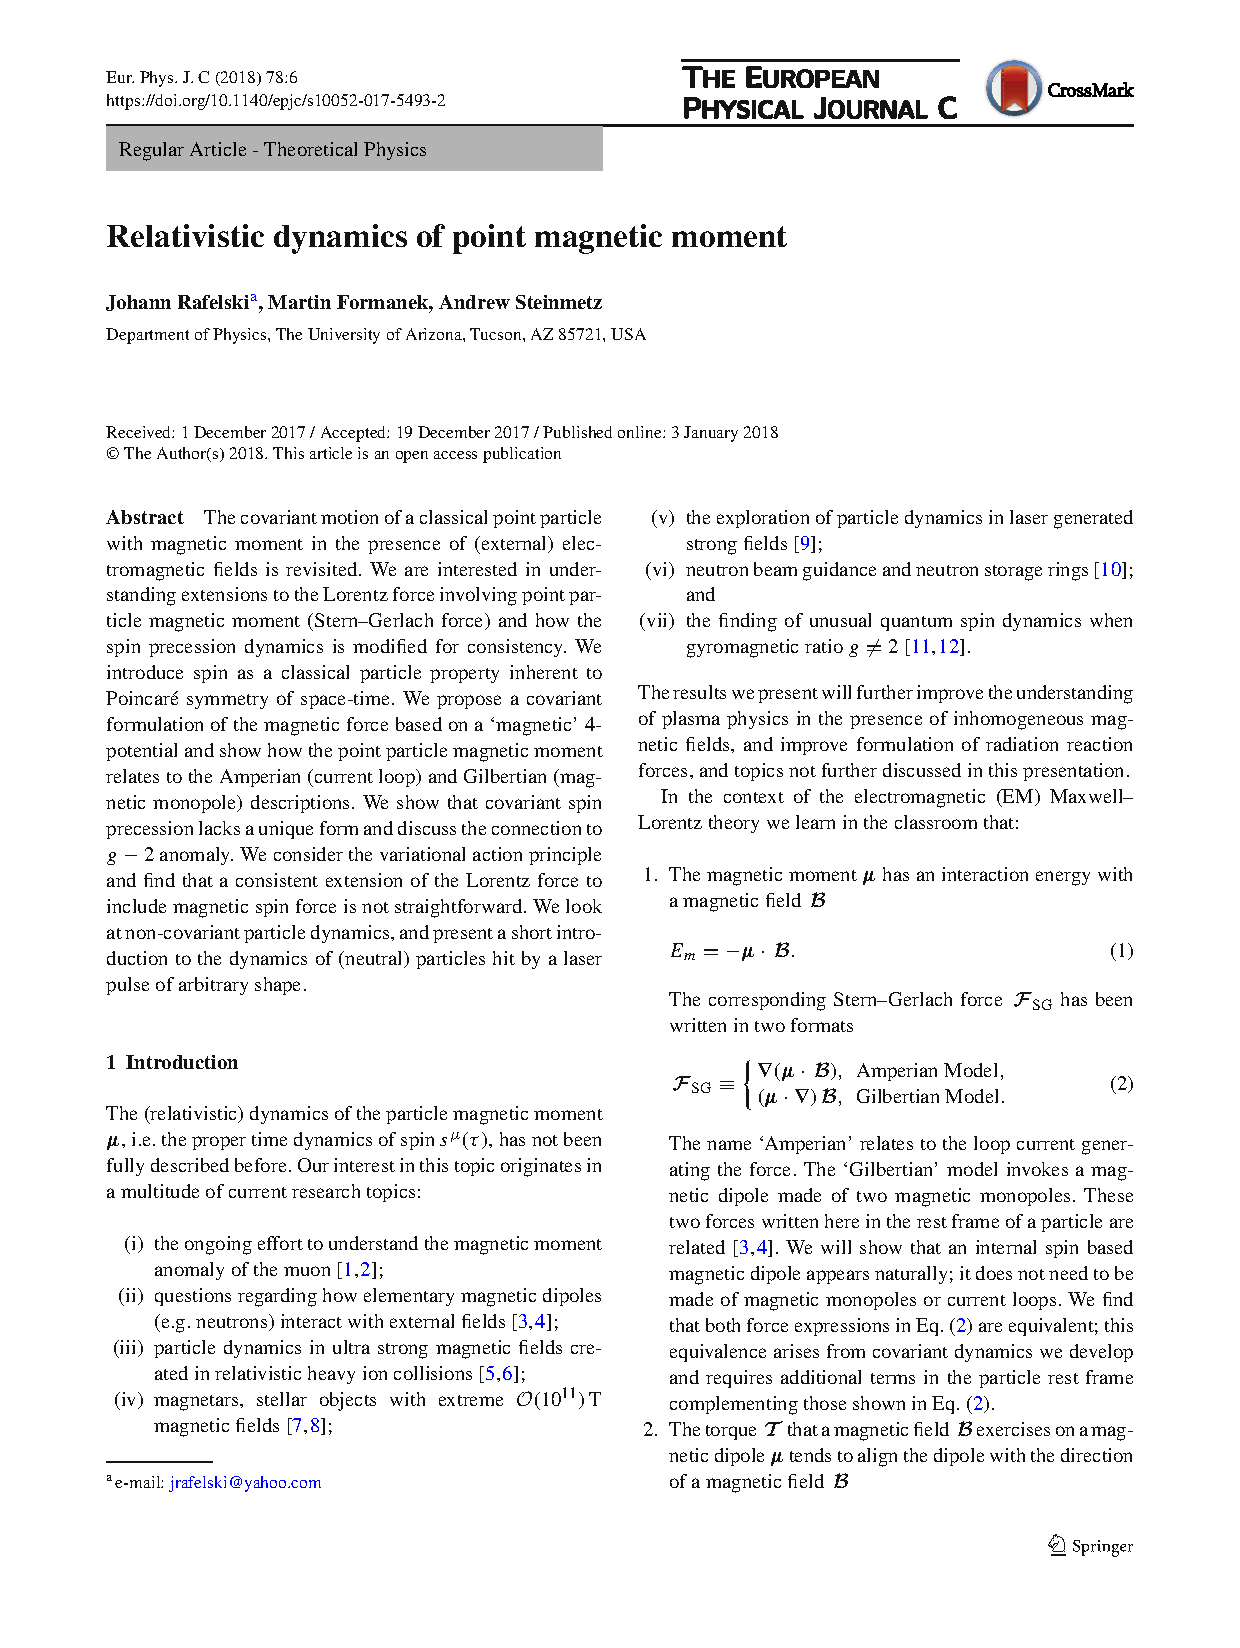
\includepdf[pages=-,pagecommand={},nup=1x2,landscape=true,width=5 in]{publications/rafelski2018relativistic.pdf}

%%%%%%%%%%%%%%%%%%%%%%%%%%%%%%%%%%%%%%%
\chapter{Strong fields and neutral particle magnetic
moment dynamics}
%%%%%%%%%%%%%%%%%%%%%%%%%%%%%%%%%%%%%%%
\begin{center}
Formanek, Martin, Stefan Evans, Johann Rafelski, Andrew Steinmetz, and Cheng-Tao Yang. "Strong fields and neutral particle magnetic moment dynamics." Plasma Physics and Controlled Fusion 60, 7 (2018): 074006.

doi: \href{https://doi.org/10.1088/1361-6587/aac06a}{10.1088/1361-6587/aac06a}

.

Copyright (2018) by IOP Publishing

This is the Accepted Manuscript version of an article accepted for publication in Plasma Physics and Controlled Fusion.  IOP Publishing Ltd is not responsible for any errors or omissions in this version of the manuscript or any version derived from it.  The Version of Record is available online at \href{https://doi.org/10.1088/1361-6587/aac06a}{10.1088/1361-6587/aac06a}.

\end{center}
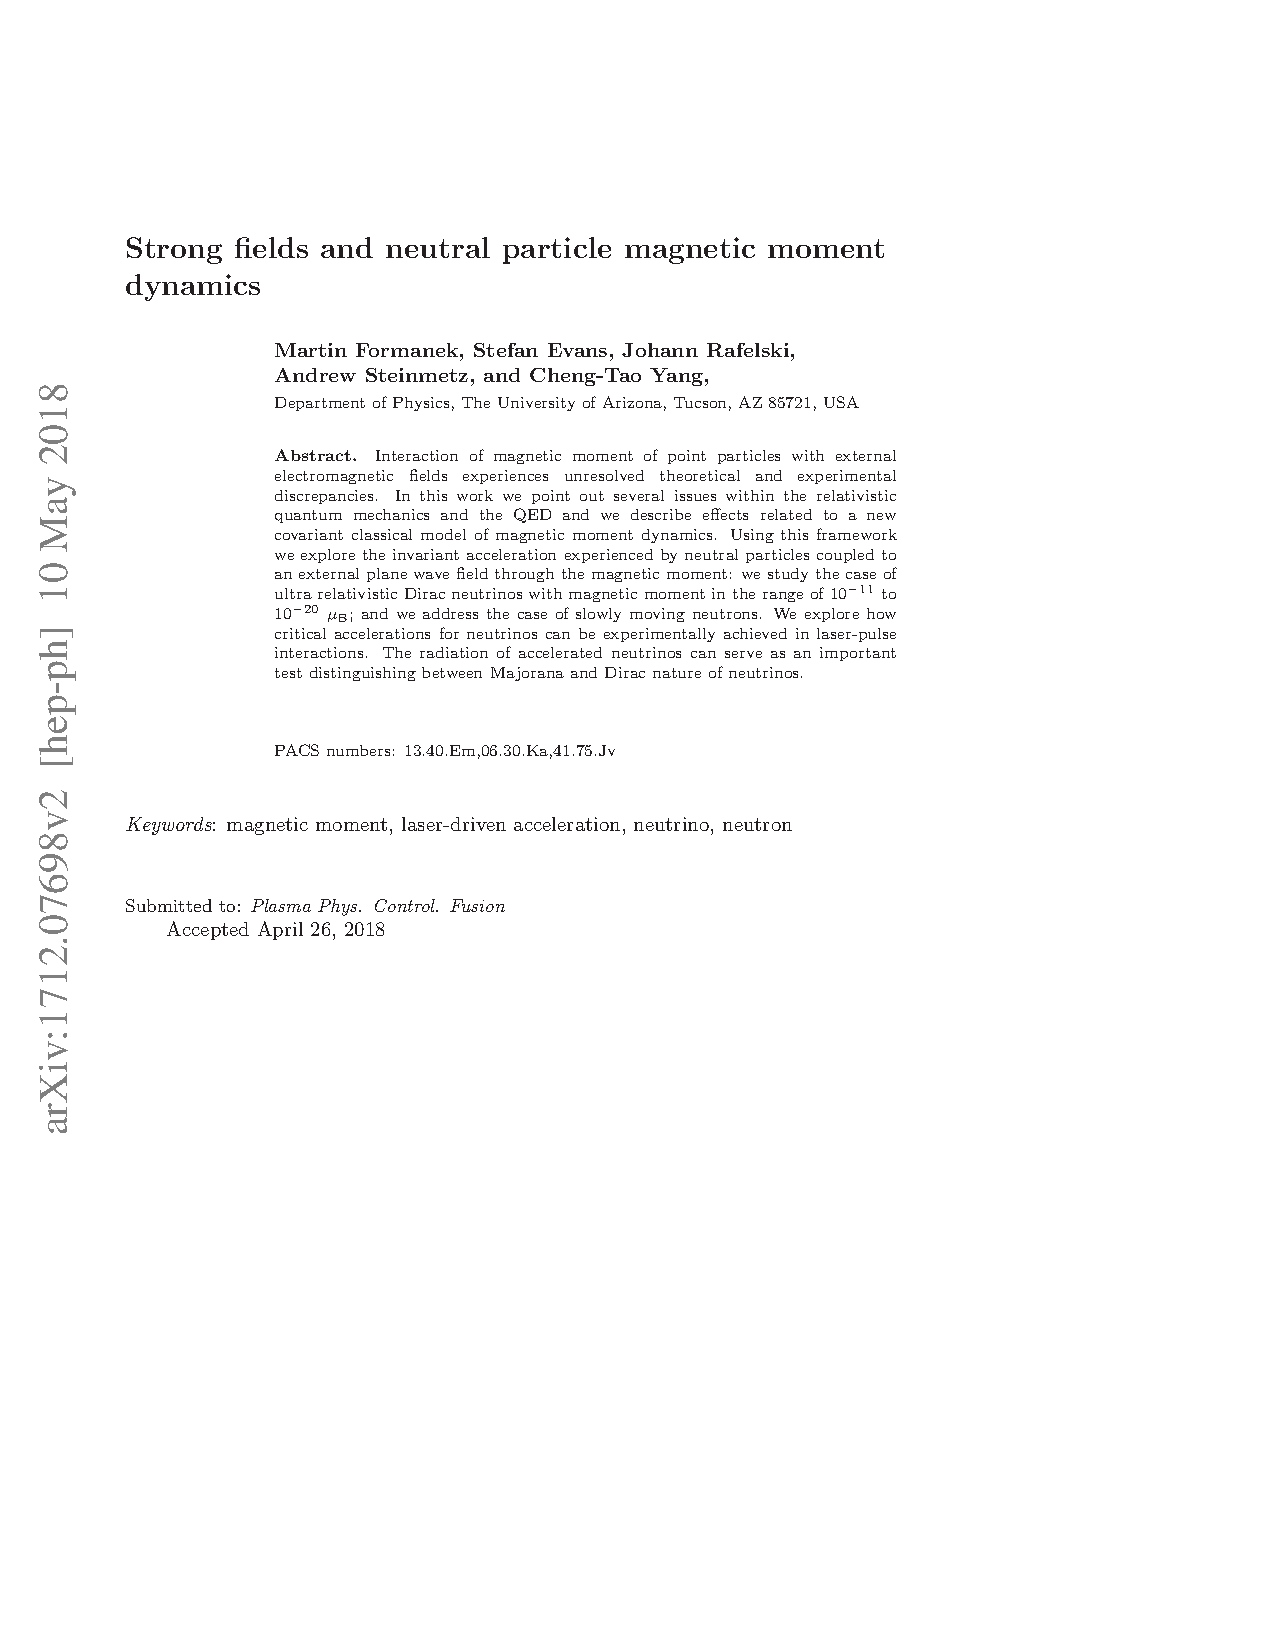
\includepdf[pages=-,pagecommand={},nup=1x2,landscape=true,width=5 in]{publications/formanek2018strong.pdf}

%%%%%%%%%%%%%%%%%%%%%%%%%%%%%%%%%%%%%%%
%\chapter{Radiation reaction friction: Resistive material medium}
%%%%%%%%%%%%%%%%%%%%%%%%%%%%%%%%%%%%%%%
%\begin{center}
%Formanek, Martin, Andrew Steinmetz, and Johann Rafelski. "Radiation reaction friction: Resistive material medium." Physical Review D 102.5 (2020): 056015.

%doi: \href{10.1103/PhysRevD.102.056015}{10.1103/PhysRevD.102.056015}

%.

%Copyright (2020) by the American Physical Society

%This article is an open access article distributed under the terms and conditions of the Creative Commons Attribution %\href{https://creativecommons.org/licenses/by/4.0/}{(CC BY 4.0)} license.
%\end{center}
%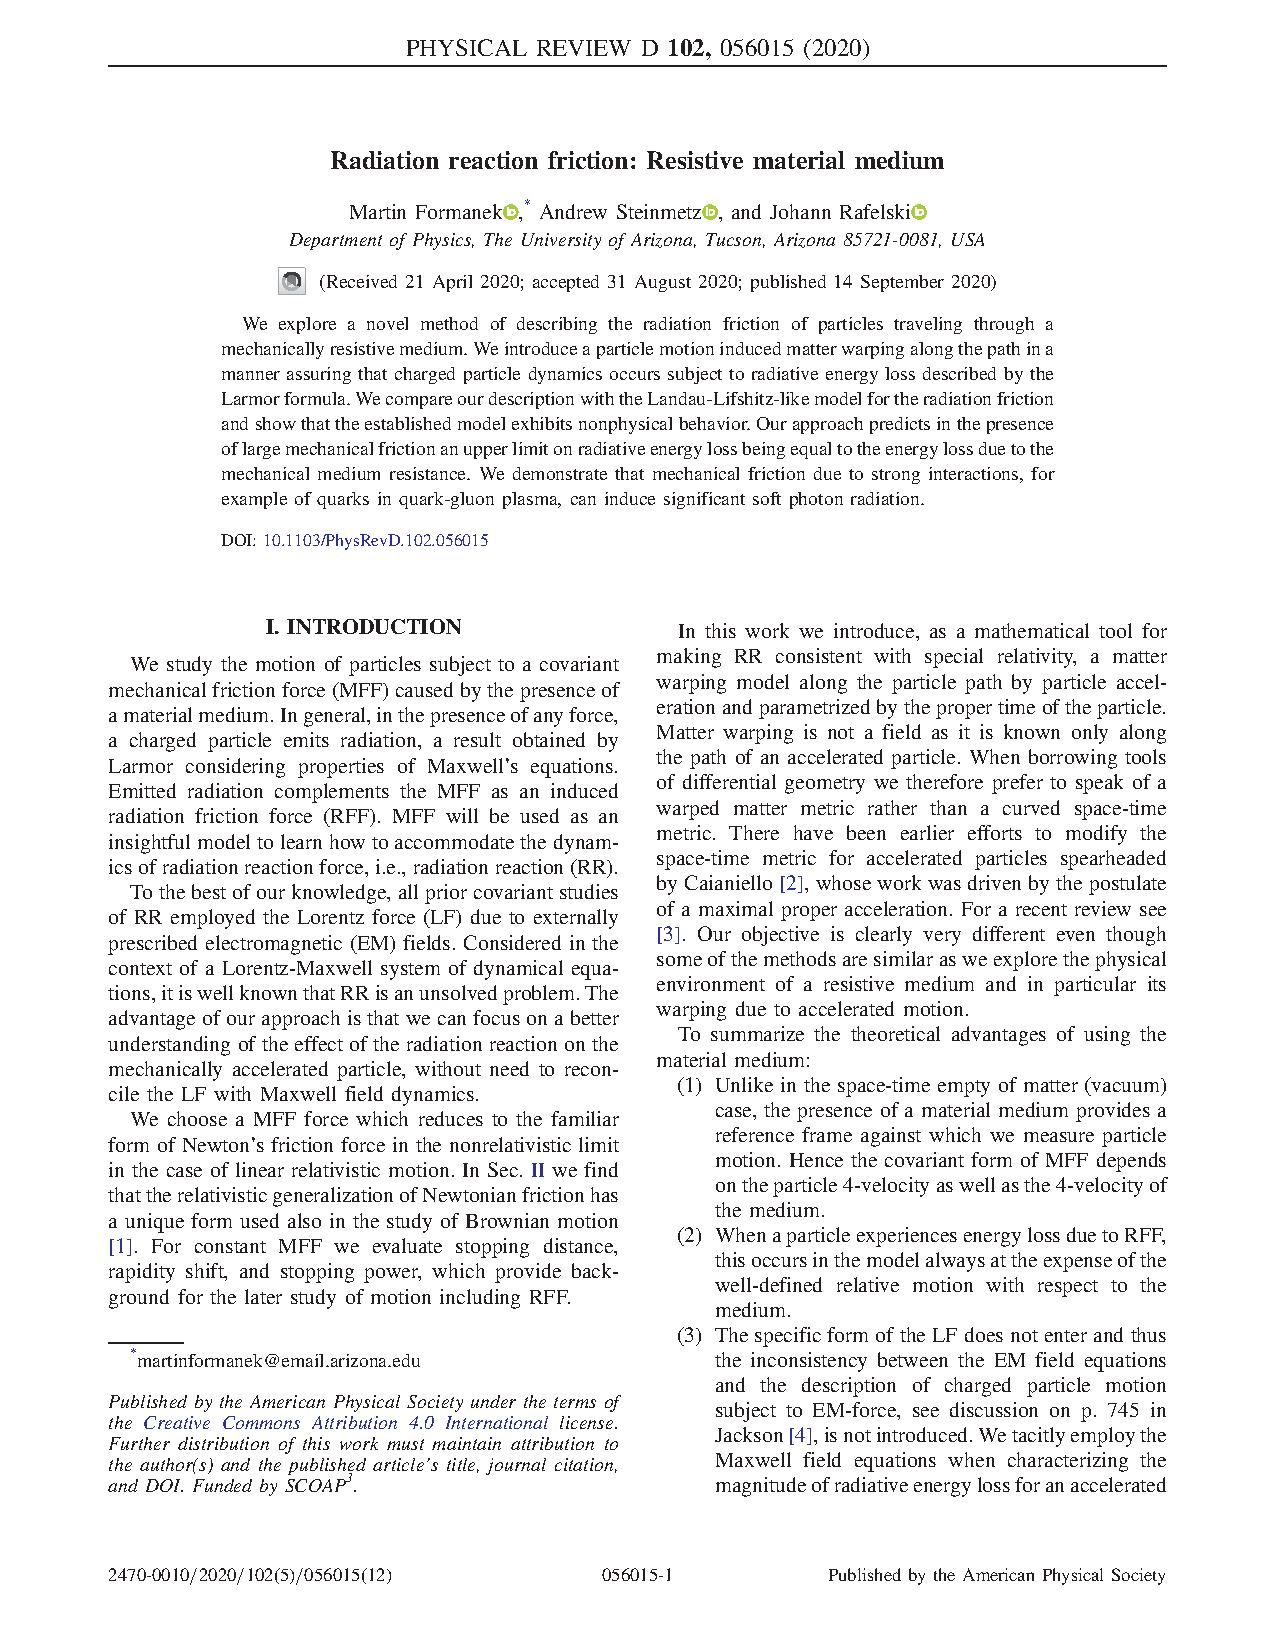
\includepdf[pages=-,pagecommand={},nup=1x2,landscape=true,width=5 in]{publications/formanek2020relativistic.pdf}

%%%%%%%%%%%%%%%%%%%%%%%%%%%%%%%%%%%%%%%
\chapter{Magnetic dipole moment in relativistic quantum mechanics}
%%%%%%%%%%%%%%%%%%%%%%%%%%%%%%%%%%%%%%%
\begin{center}
Steinmetz, A., Formanek, M. \& Rafelski, J. Magnetic dipole moment in relativistic quantum mechanics. European Physical Journal A $\bb{55}$, 40 (2019).

doi: \href{https://doi.org/10.1140/epja/i2019-12715-5}{10.1140/epja/i2019-12715-5}

.

Copyright (2019) by Springer Nature

With kind permission of The European Physical Journal (EPJ)

Reprint permission for this thesis granted under \href{https://s100.copyright.com/CustomerAdmin/PLF.jsp?ref=9a7a42d0-4511-4427-8acd-73a16083772c}{License Agreement 5600921273203}

License date: August 02, 2023
\end{center}
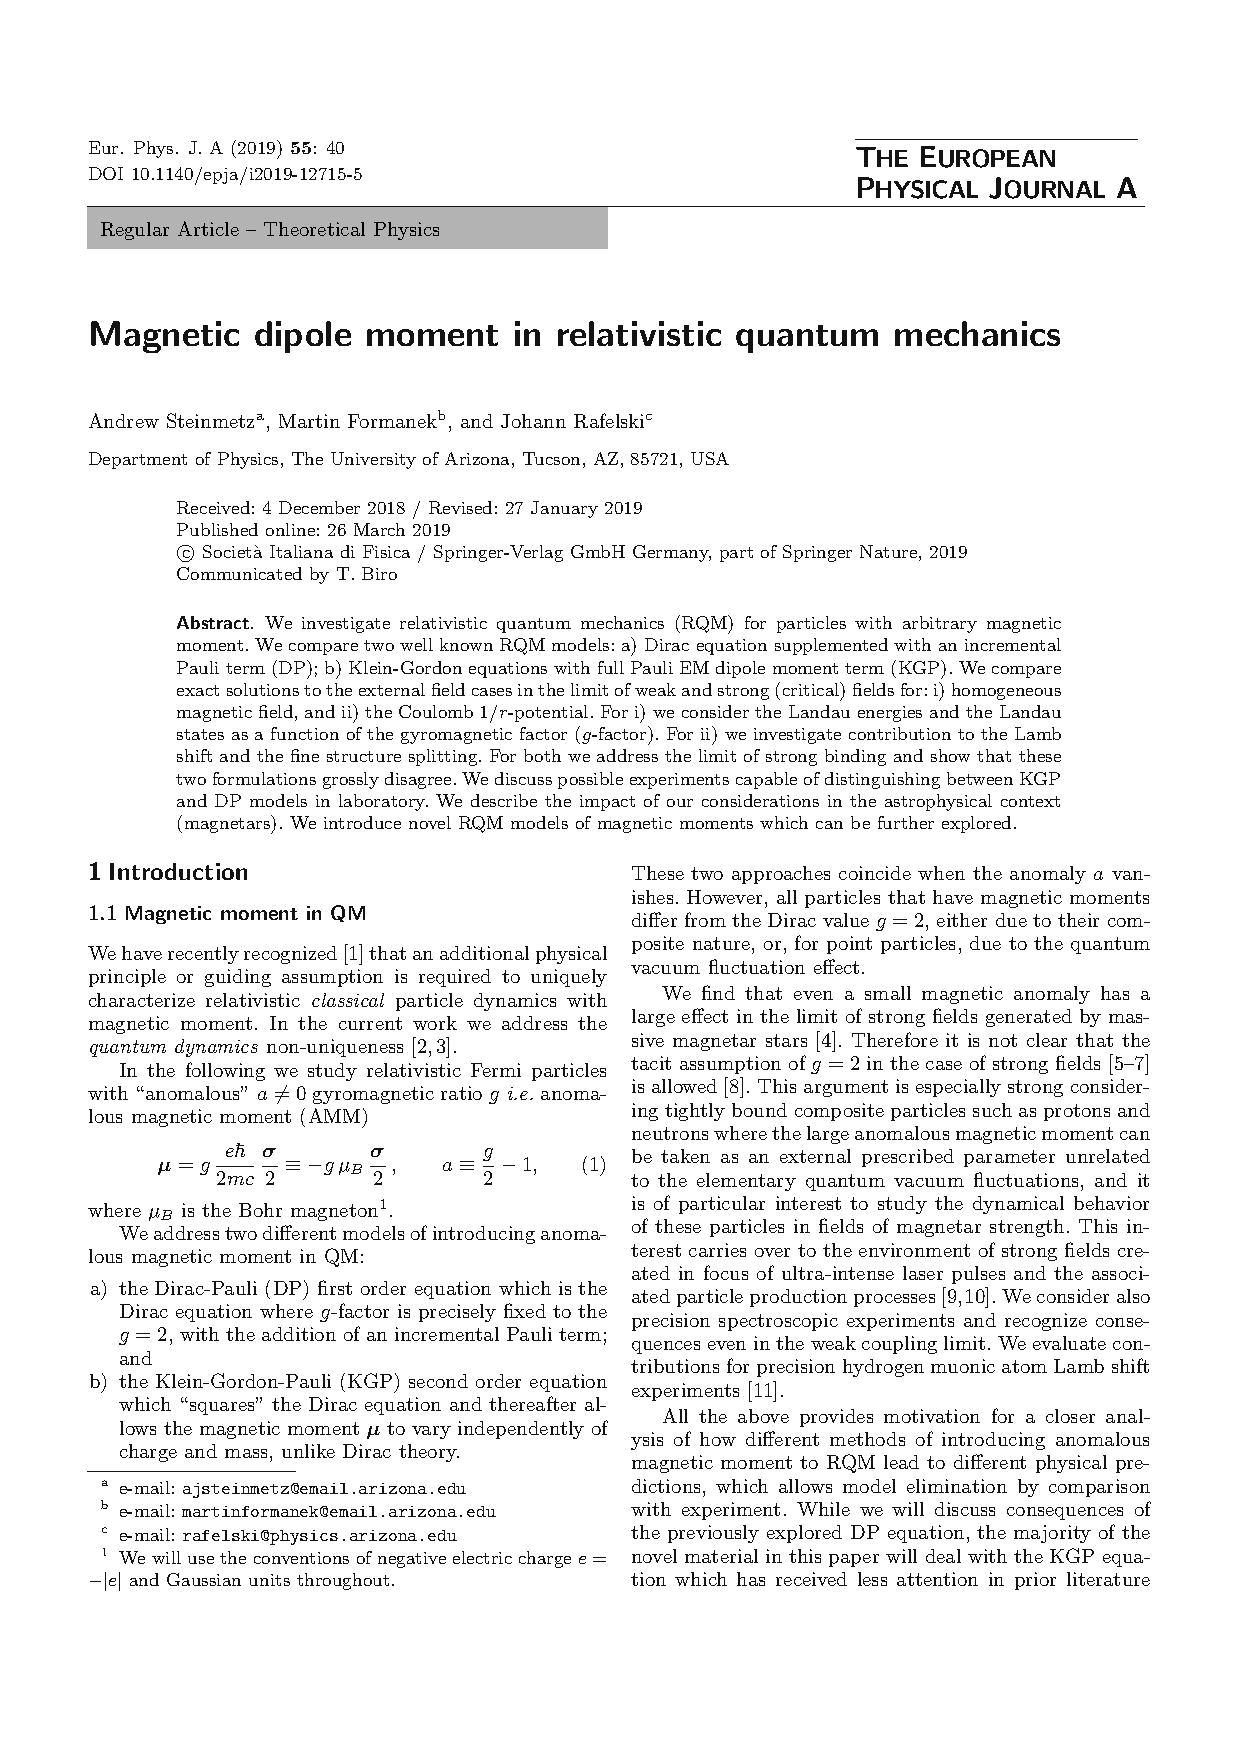
\includepdf[pages=-,pagecommand={},nup=1x2,landscape=true,width=5 in]{publications/steinmetz2019magnetic.pdf}

%%%%%%%%%%%%%%%%%%%%%%%%%%%%%%%%%%%%%%%
\chapter{A Short Survey of Matter-Antimatter Evolution in the Primordial Universe}
%%%%%%%%%%%%%%%%%%%%%%%%%%%%%%%%%%%%%%%
\begin{center}
Rafelski, J.; Birrell, J.; Steinmetz, A.; Yang, C.T. A Short Survey of Matter-Antimatter Evolution in the Primordial Universe. Universe 2023, 9, 309.
doi: \href{https://doi.org/10.3390/universe9070309}{10.3390/universe9070309}

.

Copyright (2023) by the authors. Licensee MDPI, Basel, Switzerland.

This article is an open access article distributed under the terms and conditions of the Creative Commons Attribution \href{https://creativecommons.org/licenses/by/4.0/}{(CC BY 4.0)} license.

\end{center}
\includepdf[pages=-,pagecommand={},nup=1x2,landscape=true,width=5 in]{publications/rafelski2023shortsurvey.pdf}


\end{document}
